\documentclass[14pt]{extarticle}

% Any percent sign marks a comment to the end of the line

% Every latex document starts with a document class declaration like this
% The option dvips allows for graphics, 14pt is the font size, and article
%   is the style 

\usepackage[pdftex]{graphicx}
\graphicspath{ {./images/} }
\usepackage{url}
\usepackage[left=2cm,right=2cm,top=2cm,bottom=3cm]{geometry}
\usepackage[english]{babel}
\usepackage{amsmath}
\usepackage{amssymb}
\usepackage{graphicx}
\usepackage{float}
\usepackage{enumerate}
\usepackage{booktabs}
\usepackage[numbers]{natbib}
\usepackage{amsmath}
\usepackage[ruled,vlined,linesnumbered]{algorithm2e}
\usepackage[hidelinks]{hyperref}
% These are additional packages for "pdflatex", graphics, and to include
% hyperlinks inside a document.
% !TeX spellcheck = en_US 
\setlength{\oddsidemargin}{0in}
\setlength{\textwidth}{6.5in}
\setlength{\topmargin}{0.2in}
\setlength{\textheight}{7.6in}
\setcounter{tocdepth}{4}
\setcounter{secnumdepth}{4}

% These force using more of the margins that is the default style
\newcommand{\myparagraph}[1]{\paragraph{#1}\mbox{}\\ \linebreak}
\numberwithin{equation}{section}
\pagestyle{headings}
\begin{document}
	
	\bibliographystyle{ieeetr}
	
	% Everything after this becomes content
	% Replace the text between curly brackets with your own
	
	\title{Learning Goal-Oriented Dialog Strategies using Deep Reinforcement Learning}
	\author{Shishir Narayan \\ Berlin}
	\date{\today}
	
	% You can leave out "date" and it will be added automatically for today
	% You can change the "\today" date to any text you like
	
	
	\maketitle
	\clearpage
	% This command causes the title to be created in the document
	
	\setcounter{page}{1}
	\section*{Declaration}
	I hereby declare that this thesis was composed solely by myself and that the work contained herein is my own except where specific references are made to the work of others or explicitly stated otherwise in the text. Further, I declare that this work has not been submitted, in whole or in part, for any other degree or professional qualification.
	
	This thesis contains fewer than 30,000 words including the bibliography, footnotes, tables and equations.
	\\\\
	\begin{flushright}
		Shishir Narayan\\
		\date{\today}
	\end{flushright}
	\clearpage
	\section*{Confidentiality Statement}
	This master thesis is provided with a blocking notice. Access to this thesis is not allowed to unauthorized persons or organizations. The master thesis may not be made accessible to the third party, with the expectation of the first and secondary referee as well as the members of the examination board of the SRH Hochschule Heidelberg neither completely nor in parts.
	Further, any publication, duplication or the passing on of the master thesis in parts are not permitted without the permission of the company \textit{botconnect GmbH}\footnote{www.botconnect.ai}
	\\\\
	\begin{flushright}
		Shishir Narayan\\
		\date{\today}
	\end{flushright}
	\clearpage
	\section*{Acknowledgments}
	\clearpage
	
	\section*{Abstract}
	In this work we focus on applying reinforcement learning techniques to develop simple goal oriented dialog systems. The design and development of dialog systems is known to be a challenging task, with developers spending a lot of time and effort on foreseeing prospective user interactions to develop appropriate system responses. This mapping across predicted user inputs and the correct system outputs is called a dialog strategy or in terms of reinforcement learning, a dialog policy.
	
	Here we model the design and development of this strategy as a sequential decision-making task. This is done by employing a framework known as Markovian Decision Processes(MDP) that helps to model decision-making tasks. Our task is goal-oriented or domain-specific, i.e. to assist the user in helping to sell a product to a customer. Thus our goal oriented dialog system, commonly known as a chatbot, helps the user in achieving this predefined goal by having a dialog with the user which consists of making suggestions or asking questions about the customer. According to user response and previous interactions, the system decides what to say next to help the user. The success of the system is directly dependent on the quality of the learnt policy, which is dependent on the complexity of the environment and user simulation. We use Deep Reinforcement Learning techniques which use the MDP model to learn the required dialog policies by interacting with a simulated user environment. 
	
	In this thesis we also detail the probabilistic model of the environment simulation, as well as the intricacies in casting our dialog domain as a MDP. Further, we delve in detail about the various reinforcement learning techniques and formulations that can be used to optimize dialog policies. Finally, we give a summary of deep learning before examining two reinforcement learning algorithms, Advantage Actor Critic and REINFORCE and their formulation using neural networks in detail. This is then proceeded by a documentation of the results obtained during the training of these algorithms and their comparisons with appropriate classic reinforcement learning baselines. 
	\clearpage
	\tableofcontents
	
	\clearpage
	\listoffigures
	
	\listoftables
	\section{Introduction}
	\subsection{Overview}
	Automating speech and dialog is generally regarded as one of the more difficult challenges to solve in Machine Learning, especially in the long term. As we know Language is a unique marker of intelligence in humans, in fact, theorists have suggested that crucial evolutionary developments that led to the burst in creativity and productivity in the Neolithic era were the emergence of human language \cite{macwhinne_lang_evol}. 	
	Thus, it seems our very notion of intelligence is deeply connected to language and speech. Alan Turing, in his \textit{Imitation Game} \cite{turing_mind} first attempted to define the standard of intelligence for a machine by testing whether a human participant was able to successfully differentiate between a conversation with it from a human conversation. It was he who first suggested that any sufficiently intelligent machine could simulate the process of learning of an animal or even a human child. This idea is central to our approach of using Reinforcement Learning to build a dialog system. Ultimately, the goal is to simulate the inception of a truly intelligent conversation machine, which, according to Ray Kurzweil \cite{kurzweil_sing} is only a matter of time. \par
	
	Formally, Dialog Systems are computer programs designed with the purpose of conversing with humans. These systems are generally built with a pipeline like structure in order to understand user utterances and have coherent and meaningful conversations. The primary component of a Dialog System is the Dialog Manager. This component decides what to say next to the user. The process of \textit{deciding} can involve external queries to knowledge resources such as databases and APIs and estimating the various states of the dialog. Once we have a Dialog Manager, we have a plethora of options to communicate with the end user such as speech, text or gestures.
	One of the earliest successful Dialog Systems was created at the MIT AI Laboratory by Joseph Weizenbaum in 1966. This early program was called ELIZA \cite{Weizenbaum:1966:ECP:365153.365168} and used large extended chains of simple word re-orderings to produce dialog which could imitate the language and behavior of a psychotherapist. With recent advancements in theoretical and practical applications of AI and Computing, we can confidently say that natural, meaningful and useful conversations with machines is now fully plausible. In this thesis we focus on text-based Dialog Systems, conventionally known as \textit{chatbots}. Chatbots can be broadly categorized into two groups depending on the nature of the dialog. These are \textit{Chat-Oriented} or \textit{Open Domain} chatbots and \textit{Goal/Task-Oriented} or \textit{Closed Domain} chatbots. The former type aims to generally converse with users providing reasonably contextually aware responses where the chatbot is expected to talk about anything i.e. it is an open domain setting. Goal-Oriented chatbots on the other hand are designed to help users achieve a certain task e.g. Making a restaurant reservation, rather than having a general conversation. Therefore, Goal-Oriented chatbots have narrower conversations limited a particular task or domain setting. In this work we focus on designing Goal Oriented chatbots to help as an assistant during sales calls.
	\subsection{Motivation}
	Since its inception, humanity has been leveraging technology to augment its workers with the goal of maximizing efficiency and productivity. This precept is adopted by botconnect, a startup based in Berlin that works on applying Machine Learning algorithms to automate processes in large enterprises to help empower their users with increased speed, efficiency and productivity. One field where such a project is highly valuable is Enterprise Sales. \par
	Creating individual value for customers is essential for lead generation and customer retention and in turn successful sales, which all depend on a fast decision-making process by the human sales agent. Massive amounts of data that is stored in multiple complex systems such as Distributed Databases and Customer Relationship Management (CRM) Systems make this problem increasingly difficult to solve as the organization grows. In order to generate value for a present or prospective customer, a sales-agent often has to decide what to suggest to a customer and how to do it. The varied sources, sizes and types of data often make it inefficient for the sales-agent to analyze while simultaneously trying to interpret customer behavior and preferences in a short span of time such as a phone call. Botconnect's recommendation engine, built applying Deep Learning with more traditional filtering techniques \cite{ncf2017}, can model customer preferences once trained on enterprise customer-sales data. The service is now being applied to large enterprises primarily by customer and sales agents whose daily job involves a high amount of interaction with customers and potential customers. \label{plag1} When queried with a customers identity, the service uses its trained model to generate a ranked list of recommended products for the customer, which the sales agent then uses to create offers during their interactions. Even though this solves the problem of having to dive through data manually for recommendations, it still leaves open the issue of having to come up with a reasonably good dialog strategy to successfully convert the conversation to a sale.\par  \label{plag10} 
	The entire cycle of a sales call, from greeting to making a sale is what we propose to automate in a manner that is clear, interactive and effortless for the agent to use \cite{frey2017future}. We aim to accomplish this by having a dialog \cite{Tao_of_CHI} between the sales-agent and a dialog system that augments the powers of the agent. Thus we propose a second dialog between the agent and sales bot which would  occur simultaneously as the agent interacts with the customer. This Dialog System is built using best practices in handling sales dialogues and trained with a large amount of agent-customer interactions with the help of a simulated agent to come up with a good dialog strategy for the current situation. This Dialog System combined the recommendation service provides auxiliary support to the agent, augmenting their capabilities and maximizing the chance of a successful sale. \par
	Classic Spoken Dialog Systems are in general formed by components such as a Dialog manager, modules to understand and generate spoken language as well as a speech synthesizer for the audio and an analyzer for text-to-speech. In our case we focus on a text based dialog system, this is a simpler system consisting only of a User Simulator, a Dialog Manager and a chatbot based User Interface. Thus the primary motivation and aim of this project is to design and implement a Dialog Manager trained with Deep Reinforcement Learning Techniques that can learn a good internal dialog policy based on interactions with a Simulated User and with Input from the recommendation Service. This policy is a sales dialog strategy that the system uses to help the agent make successful sales. This learned policy is then used by the system to determine its response at each dialog turn.
	\subsection{State of the Art}
	In the past three decades the design of Goal Oriented systems have been under constant development and has changed drastically with the introduction of new techniques such as deep learning. Due to these changes there have been several new frameworks proposed for Dialog Management. One of the first commercially successful Goal oriented systems was JUPITER \cite{zue_jupiter}. Created in the 2000s, this system was designed with a hand-crafted approach to modeling dialog states with the purpose of helping users retrieve worldwide weather forecast information via dialog over the telephone. Another milestone in this field was the introduction of the Information State modeling paradigm \cite{Larsson:2000:ISD:973935.973943}. In this work the authors proposed a complete framework for Dialog State Tracking.
	Recent important attempts in creating such machines is documented below. These systems can broadly be categorized as following.
	\subsubsection{Dialog Policy trained with Reinforcement Learning}
	Applying Reinforcement Learning to Dialog Systems has recently seen an explosion in research activities with the arrival of Deep Learning coinciding with wide availability of cheap and powerful computing resources. In RL typically the main objective is to learn a good approximation of a function mapping the states of an environment to actions and deep neural networks have been shown to be excellent approximators for this purpose. In this field the concept of a Markov Decision Process (MDP) is at the core. The details of an MDP and how to design and solve it are discussed in later chapters. An MDP is a mathematical framework that facilitates the learning of an optimal mapping between situations that arise in a dialog (otherwise known as states of a system) and actions(or system responses)\cite{mdp-bellmann}. Levin, Pieraccini and Eckert back in 1998 were the first to formally compose the problem of dialog management as an MDP \cite{mdp-pieraccini} and in turn, laid the foundation for the future.
	
	Once we have the MDP of a dialog, it is simply a matter of applying one of the many Reinforcement Learning Algorithms to learn the most optimal mappings between states and actions and thus select the best action of a given state. This was the focus of the work done in this field in the next decade \cite{Young99probabilisticmethods}\cite{Singh_mdp}\cite{Pietquin_mdp}. This however solved only the problem of dialog policy estimation. But to build a complete dialog system, as research in the past decade has shown, a complex structure with multiple components that are able to comprehend human input and extract the state of the dialog, select an action or dialog act as a response to this state and finally translate this into human language. Formally these components are known as  a Natural Language Understanding Unit (NLU) and a Natural Language Generation Unit, Dialog State Tracker and Dialog Policy Learner. A novel application of RL using this architecture for the purpose of Information Retrieval was shown in \cite{Dhingra2016EndtoEndRL}, where the authors built a dialog system to help users search knowledge bases for movies with simple queries. In the following year Cuayáhuitl designed and implemented a robust dialog system for the restaurant reservation and booking domain \cite{Cuayhuitl2016SimpleDSAS}, where the author successfully uses simple noisy text input from the user and the previous history of the dialog to represent a so-called \textit{belief-state} that is an estimation of the true dialog state. Recently, the authors in \cite{Li17e2eDS} designed a complex dialog system to work in the movie booking domain. This robust system worked with raw user input and thus used a NLU to process inputs and build an internal \text{belief state} representing its estimate of the true dialog state. The NLU they used is a commonly one that is proposed in \cite{HakkaniTr2016NLU}. The NLG unit for their Dialog System was implemented from \cite{Wen_NLG}. Both the NLU and the NLG use Long Short-Term memory units which form a type of Recurrent Neural Network \cite{hochreiter1997long}. For training the dialog policy the authors also used a Simulated User with a hidden agenda and goal \cite{Schatzmann_agenda_sim}\cite{Li_user_sim}. The dialog policy was trained using Deep Q Networks \cite{Mnih_DQN}.
	\subsubsection{Dialog Policy trained with End-to-End Supervised Learning}
	Even a decade ago the use of deep neural networks was restricted to the academia and veterans of the machine learning industry with access to a large amount of resources. Now, with the arrival of deep learning and consequent theoretical breakthroughs, wide availability of cheap computing resource companies such as Google building tools like Tensorflow\cite{tensorflow} making it easily accessible to anybody with a computer. It is being applied in every possible field of human endeavor. This also means that neural networks have also been used to design dialog systems. In this case, it is not in the sense of representing a policy or an NLU, but completely from scratch. It involves coming up with a neural network based dialog system that once trained, does everything from understanding the user input semantics, deciding the state and converting the semantics of the desired output to speech or text. This is what is meant by End-to-End. One pioneer in this field was Sutskever, who in 2014 proposed the \textit{Sutskever Model} \cite{Sutskever_seq_2seq}. The author used recurrent neural networks(RNN) to first learn sequences of user and system responses from a large amount of training data. This model has also come to be known as the \textit{encoder-decoder model}. The architecture is made up of two separate components built with RNNs: the first analyses the input sequence and encodes it into a feature vector, the other, then decodes the feature vector to output the predicted semantics of the sequence. Using this, the dialog manager is able to predict the latent dialog state. The disadvantage in this case, is the large amount of time and resources needed for training a large neural network and a painstaking preprocessing, labeling and restructuring of the training data.
	
	RNNs are important in this field of dialog systems and are used widely. This is mainly due to their ability to perform very well on sequence and temporal processing tasks \cite{karpathy_rnn}. This is because RNNs have a feedback loop that functions as a very small memory storage and allows it to capture time based information about the data flowing through it by rolling out the time layers as individual feed forward layers. This feedback loop can also become arbitrarily large and lead to the \textit{Vanishing Gradient Problem}\cite{hochreiter1998vanishing} which can be overcome by using LSTMs\cite{hochreiter1997long}. Another landmark project was proposed by Bordes and Weston, who recently used the \textit{Sutskever Model} but replaced RNNs with End-to-End Memory Networks\cite{Sukhbaatar_end2end_mem_net}. They are a modified form of RNN combined with external memory that have the ability to manage very long term dependencies, forget unimportant information and can be trained end-to-end. This was a comprehensive goal-oriented chatbot and built using the BabI tasks\cite{babl} for the domain of restaurant reservation\cite{bordes_weston_e2e}. This system is state of the art and demonstrates powerful abilities such as being able to interpret, remember and update past user preferences and decisions.
	\subsubsection{Dialog Policy trained with a Combined Approach}
	One of the primary disadvantages in using reinforcement learning to learn sophisticated dialog is that it involves the training of not just the dialog policy but auxiliary components such as the NLU and NLG. This is very compute intensive and is difficult to optimize the model. Further, this optimization is typically often be done on simulated users with developer designed user responses as using real users is often impractical and costly, therefore the trained model may not represent the nuances and sophistication when dealing with real user responses.
	Although some of these could be overcome with the use data driven user simulation, this approach is generally less data intensive.
	On the other hand supervised learning typically requires a very large amount of training data. This training data must have sequences of real human to human interactions from which the system could learn. For Goal Oriented chatbots, which are often designed for a specific domain, this kind of training data is seldom available. To overcome these limitations a third branch of dialog system optimization was born. This method, also known as a hybrid approach to dialog policy optimization combines both the above approaches to arrive at dialog systems trained with the sophistication and nuance of real human dialog along with the granular component training offered by RL. In their work to product a robust dialog system for the domain of restaurant information and booking, the authors in \cite{Su_continous_dm} propose a multi-phase approach to training the dialog policy. The design begins with the building of a \textit{Policy Network}, which is a neural network with a single hidden layer. The output of this layer is the actions that the policy can take and the input is the belief state given to it by the DST. Once they built this, the authors used the Wizard-Of-Oz corpus to train the policy net in a fully supervised fashion, this was phase one. In the second phase the authors then used a variant\cite{Schulman_trpo} of RL based algorithm known as Policy Gradients \cite{Sutton_pg} combined with the concept of Experience Replay\cite{Lin1992} which reuses previous experiences in a supervised manner to optimize the policy net to maximize the expected cumulative reward and further explore the dialog space. Recently another such system was introduced by Williams, Asadi and Zweig who proposed the concept of Hybrid Code Networks\cite{Williams_HCN_e2e} which  also address the drawbacks of the above approaches. The authors again describe two distinct phases of learning for the dialog policy. In the first, they train an RNN with domain specific, hand-crafted feature templates comprised of system actions. Once the model is trained, they then put the dialog system online and use a vanilla policy gradient\cite{Sutton_pg} approach to fine-tune the model with real user interactions. 
	\pagebreak
	\section{Dialog Systems}
	\subsection{Overview}
	In this section we want to give the reader a brief introduction to the semantics, components and architecture commonly found in the field of dialog systems. From literature, it can be seen that depending on the type of application domain, user utterances and required system responses vary significantly. The two most commonly found varieties are speech based dialog systems, known as spoken dialog systems and text based dialog systems, known as chatbots. As we know, these systems can be further grouped into Goal Oriented (GO) or Open Domain chatbots. In this work we primarily focus on Text Based GO Dialog Systems. Here, it is a good idea to discuss what exactly we mean by dialog and some other assumptions that we make in the process of designing a Dialog Manager. A dialog, in our case, is a process of sequential and turn-based exchange of information between only two participants, using only a word or a string of words (a dialog act) at each turn. Another assumption we make is that the above described dialog can, in principle,  be represented as a Markov Decision Process \cite{mdp-pieraccini}. This is further elaborated in Section \ref{subsec:mdp}. Further in this chapter we elaborate on the general architecture of a dialog system followed by focusing on prospects of Dialog Management and User Simulation and end with some popular applications of such systems.
	\subsection{System Architecture}\label{subsec:sys-arch}
	It is well known and can be seen from the literature \cite{ds_survey} that there is no standard architecture for designing dialog systems, but in general they can be said to be made up of two distinct components. The first is an internal dialog management unit which, depending on the approach used (RL or Supervised), may or may not consist of components to process and generate natural language. But this unit must include a dialog policy learner and a dialog state tracker, although these could be the same component, i.e.\ a single neural network. Another component is the user or a simulated representation of a user for the system to interact with. This idea was first conceived by Pieraccini \cite{Pieraccini2006WhereDW} and most systems follow the described pipeline based system. The pipeline architecture for GO text based dialog systems can be seen in Figure \ref{sys-arch1} along with the flow of information. The dialog starts with a user utterance, this is then processed by a Natural Language Understanding (NLU) Component that extracts the perceived semantics of the input. These semantics represent the intent of the user and the current context which includes the previous history of the dialog. The user utterance semantics then flow into the central decision-making module called the Dialog Manager(DM). The DM interprets the input from the NLU Component in the context of the entire history of the conversation and estimates the current dialog state. This process of tracking the state according to user input is done by the Dialog State Tracker(DST) component of the DM \cite{ml_dst_review}. The other sub-component of the DM is the Dialog Policy, which takes the state from the DST as input and uses it to select the most appropriate action or system response. The semantics of this chosen action is then fed into the NLG Unit, which generates an appropriate sentence for the end user. This is the entire process of the commonly used Pipeline Architecture.
	In the next sections,  we go into further details of the Dialog Management and User Simulation component from the perspective of the current working requirements.
	\begin{figure}[H]
		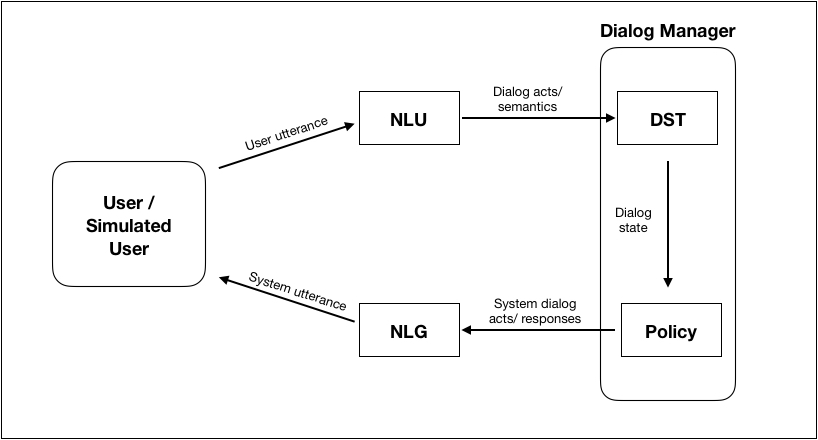
\includegraphics[scale=0.55]{sys-arch1}
		\centering
		\caption{Text Based Dialog System Architecture
			\label{sys-arch1}}
	\end{figure}
	\subsection{Dialog Management}
	The DM can generally be seen as the central decision making module of the entire system. This central component is responsible for the tracking and estimation of the current dialog state as well as choosing the best response for the user, based on the dialog state. The former is performed by a sub-component known as the Dialog State Tracker (DST)
	\subsubsection{Dialog State Tracking (DST)}
	Dialog is a sequence of turn-based interactions. This implies that the probability of a specific utterance is conditionally dependent on the sequence of previous utterances or the dialog history and the uncertainty in the mapping between the perceived input signal to its semantics. Thus, to infer the current dialog state, it is important for us to consider the previous sequence of utterances and states of the system. We can extend this to what is known as a Markovian representation of the dialog \cite{mdp-bellmann}\cite{mdp-pieraccini}, where the dialog state is fully described by the previous history of dialog states and utterances. This is a simplification of the dialog, where we have to reduce the entire state space to a unique finite set with discrete states for every possible conversation sequence. This set of discrete states can also be represented as nodes in a conversation graph. A dialog sequence is a specific path through these nodes. This process of state factorization depends on how closely the observable raw user input represents the true observable state of the dialog and it is the main function of the DST. This discrepancy can arise practically due to various factors such as noise, ambiguous user responses or changes in user goals. A few commonly found methods of state factorization for DSTs are discussed below.
	\myparagraph{Information State DST}
	These trackers are also known as rule-based and are generally found in finite state systems, where there exists a state transition network whose nodes represent different dialog states. Here the next state is a function of the latest user response and the previous state. Thus the dialog state is managed by traversing this finite state network \cite{Sutton-introRL}. Larson and Traum in \cite{Larsson:2000:ISD:973935.973943} made major contributions to this are of research with the introduction of the \textit{Information State Paradigm}, which formalized the representation of a state as a discrete random variable representing its position in the network to build a complex dialog system. This approach is convenient since no training data is required, as the state to state transition probabilities, domain information and dialog actions that is to be learnt from the dialog data are built into the hand crafted state transition network. However, a drawback is that the system does not sufficiently consider the intricacies present in natural language.
	\myparagraph{Generative DST}
	Other attempts to solve the discrepancy problem involved the use of so called \textit{generative models}. Such models are commonly found in the field of Statistical Modeling and consist of using a Dynamic Bayesian Network (DBN) to estimate the joint probability distributions between the current observation of the user utterance and the dialog state \cite{Young_dst_dbn}. Here the tracker works by representing user utterance $u$ and the true dialog state $s$ as unobserved noisy random variables. Bayes Theorem is then applied to get a distribution over $s$ dependent on the system action $a$ and the noisy user utterance $u$ and the previous state. Thus, with the DBN we can then infer a probability distribution over the state and user utterance, i.e. if $aˆ'$ is the current system action, and $s$ is the previous dialog state. Then, the model tries to estimate the joint distribution $sˆ' = P(aˆ',s)$, where $aˆ'$ is again dependent on the previous user utterance $u$. Early methods used an information state approach with discrete dialog states\cite{roy2000spoken} which became intractable with very large state spaces. To overcome these, a number of methods were put forth to approximate the dialog state \cite{Henderson:2008:MMP:1557690.1557710}\cite{Young:2010:HIS:1621140.1621240}. This also allowed the developer to optimize using domain specific feature parameters, which could be trained with dialog data.
	\myparagraph{Discriminative DST}	
	Generative models, though advantageous and relatively easy to implement, have a few drawbacks.  They use a BDN, which tries to model all complex relationships present in the input features and hence they face some difficulty in exploiting useful contextual parts of the dialog history as they are not included in the feature parameters of the DBN. This and some other important disadvantages can be found in \cite{generative_dst_limitation}. Discriminative models try to overcome these drawbacks by trying to directly model a distribution over the dialog states, given input features which are semantic representations of the dialog history. The parameters of this modeling are generally optimized using machine learning techniques such as using a Conditional Random Field (CRF). A linear-chain CRF could be utilized for learning the distribution and tracking the sequential dialog as shown by the authors of \cite{Lee2013StructuredDM}. Recently, RNNs have shown to be very effective in dealing with sequential user input to dialog state approximation \cite{Henderson2014WordBasedDS}\cite{Henderson_dst_2014}. It can accurately model a conditional distribution given even a noisy semantic dialog history. This is made possible due its ability to perform well on tasks involving sequential data. This approach is also known as a word-based DST and can be applied directly to noisy user input semantics and uses the n-gram approach combined with slot-value pairs with generic or \textit{delexicalized} features to come up with the semantics of user input after which the RNN is applied to distinguish different states\cite{DBLP:journals/corr/MrksicSWTY16}. This DST has a few major advantages such as avoiding the need for designing hand-crafted features for the input while also omitting the need for a separate NLU component and hence is widely used in the field.
	\myparagraph{Our Approach}	
	In this work we use a Information State model for the DST Component. In our domain,  the dialog is required to be structured as a conversational graph with nodes representing various states and the connections between them representing actions. This means that all our user responses are constrained by the given generic response actions,  for e.g. \textit{yes}, \textit{no}, \textit{not sure}. Since all the nodes are unique states, the path to any one state is unique. This is the same as the State Transition Network described in \cite{Sutton-introRL}. Therefore our model uses the Information State Paradigm i.e.\ employs a full MDP \cite{Larsson:2000:ISD:973935.973943}. Here, any state with the latest user action contains all the information required to infer the next state. This representation has a few key advantages in our case. The first being that it allows us to model the dialog as a full MDP, which means we can easily apply RL Planning and Control algorithms to solve it \cite{Sutton-introRL}.  The second key advantage is that with this representation we do not need an explicit NLU, as there exists a one to one mapping between the observable feature vectors (user input and observed dialog state) and the true dialog state. Since we use a deep neural network to model the policy, using this representation lets us easily generalize between similar states in large state-action spaces. This approach to DST design also requires very less data to train, which lets us effectively add, change and test domain specific features quickly and without changes to the dialog system.
	\subsubsection{Dialog Policy} 
	Previously we saw how given the history of the dialog we could infer the current state. This state is representational of the current context of the conversation, previous user and system responses and in some cases the user's needs and intentions. Intuitively, the next step is to choose how to respond to the users latest utterance with the most appropriate dialog act. This is the job of the dialog policy, the \textit{brain} of any dialog system. The behavior of this module is of crucial importance to the success of the entire system as it plays an intermediary role between the system and user, thus playing a role in the quality of the user experience. This behavior is controlled by the semantic mapping between the dialog states and system actions. This mapping in essence, has to be learnt and the best policy would be one where the user reaches his goal in the least amount of time, which can be achieved efficiently using Reinforcement Learning. 
	
	In RL we work by modeling the abstract way animals behave in nature. This means that we have some agent acting in an environment. The agent can observe a certain state at a time denoted by $s_t$. The agent, depending upon the observed state then chooses an action $a_t$ to perform in the environment, this chosen action is based on a certain policy it has learned from past experience. The nature of the experience whether positive or negative, is determined by a reward $r_t$. Finally, the action taken changes the environment which is now in state $s_{t+1}$. In this manner, the job of the DM is to learn the most optimal policy for orchestrating efficient and useful dialog. This means, in terms of RL, the dialog policy with the maximum cumulative future reward received. Thus, we make the agent maximize the cumulative future reward. The theory of RL \cite{Sutton-introRL} offers many methods to achieve this\cite{DBLP:journals/corr/abs-1711-01731}, which will be discussed further in the coming chapter. \par
	For management of the dialog interaction, one approach, as discussed before is to represent the dialog using the information state technique as a dialog tree. Other approaches generally involve the use of probabilistic models to model the noise in the observations and map them onto a distribution over actions. These are generally used in systems that require inter-domain functionality\cite{henderson_interdomain}. The advantage of using these techniques is that whichever method we use to model the DST, the function approximation technique we use to represent the policy can remain the same. This allows us flexibility in testing different hyper-parameters for optimizing the policy without modification to the rest of the system.
	\myparagraph{Our Approach}
	In this work when modeling the dialog policy using RL, the ultimate goal of the policy is to predict the best sequence of system actions given the current  state (from user input) to maximize the future reward.
	Here, the reward is determined by the success of the dialog, whether the dialog, in this instance, actually helped the sales-agent to make a sale. In our case the first inference from the DST, directly represents the dialog state input to the policy, hence the problem can be represented by an appropriate MDP \cite{mdp-pieraccini}. This is advantageous as we can feed the output of the DST, which represents the dialog state, directly into the policy net without further modifications.
	\subsection{User Simulation}
	In the process of designing dialog systems, it feels intuitive that we should use real users for testing, training and optimization. This would give the best benchmark for its quality. While it is true that this is the most ideal scenario, unfortunately for practical, real-world use cases the learning of a good policy often required thousands of dialog iterations. This makes learning from only real user interaction highly impractical mainly due to large financial, legal and time costs associated to employing human participants. Another common situation that arises when designing dialog systems, is the system designer might want to try out different representations of the dialog state. This is a problem when using a corpus of dialog data, as the entire dataset often has to be annotated again for training, which is generally a long and time-consuming process. A good solution to overcome these issues is to use a simulated user or a dialog simulation. Once built, these simulations can then be used to produce a potentially unlimited amount of training episodes or conversations, thus the dialog policy has a lot of data to learn from. Further, they can also be modified easily to experiment with several different action and state factorizations.
	Simulation of dialog according to literature, can be performed at different levels of detail. Generally these levels can be classified as raw speech signals or at the acoustic level \cite{lopez-cozar-simulation}, at the word level and at the dialog act or Intention level. Generally, this simulation is done at the dialog act level to train goal oriented dialog systems. This is due to the fact that dialog acts can be easily abstracted into its semantics representing the dialog state, which in turn makes it very efficient to train RL agents.
	There exist many different techniques of simulating a user for dialog policy optimization \cite{Schatzmann_stat_user_sim}. We discuss a few important and relevant techniques below
	\subsubsection{Rule Based Simulation}	
	These techniques are straightforward as they are simply a set of rules that dictate how the simulated user acts. This type of deterministic behavior can be inferred from the correctly annotated dialog corpus or explicitly hard coded by a developer. Some previous work that successfully applied explicit rule based models, to generate simulated dialog at a low level of granularity, can be seen in  \cite{Chung_user_sim}\cite{Lopez-Cozar_user-sim}. Here the authors used a heuristic model to generate responses at word and intention level respectively.
	\subsubsection{Probabilistic Model Based Simulation}	
	A crucial drawback in the Rule Based methods described above, is that they are inflexible and rigid with respect to simulating the uncertainty and noise generally displayed by real users. The hard coded rules generally tend to produce a high amount of variance between real and simulated user behavior and this results in a sub-optimal dialog policy with a lot of room for improvement. To overcome some of these drawbacks, a probabilistic model was proposed. In these models we would use a probability distribution to select the user responses. Early versions of this was called the bi-gram model and it was represented by the conditional probability $P$ of user utterance $u_t$, given that the current state of the system was $s_t$ is given by $P\big(u_t|s_t\big)$. This model can be widely found in literature \cite{Cuayhuitl2006LearningMD}\cite{levin_mdp}\cite{4430164}. This model was later extended to n-grams with $n$ varying from two to five in \cite{Georgila2006UserSF}, further the authors also proposed producing simulation based on a combination of linear feature vectors representing the user dialog state $s$ with user action $a$ with the probability $P\big(a|s\big)$. Other attempts in this field include the use of Hidden Markov Models (HMM) in \cite{Cuayhuitl2005HumancomputerDS} where the probability of an utterance is given by $P\big(u_t|q_t,s_t\big)$ where $q_t$ are hidden states in the weights of the HMM and the current state of the system is $s_t$. Another extension of this model was to add the concept of a user goal so that, user responses can now follow a user goal. This was proposed in \cite{Scheffler_sim} to introduce a pre-defined user goal $g$, which is generally represented as a collection of slot-value pairs. This was later modified to include a user agenda and a goal with the hidden user agenda represented by HMMs \cite{Schatzmann2007StatisticalUS}.
	\subsubsection{Our Approach}
	In this work, we use a vanilla probabilistic simulation model that is similar to the bi-gram model, but also combined with the the finite state-network representation of states based roughly on \cite{Scheffler_sim}. In practice these distributions are spread across state-action combinations. This gets converted to a collection of state-state transition probabilities, when producing simulated responses.
	\subsection{Applications}
	Goal Oriented text based dialog systems are widespread and used in many practical applications and industries. These dialog systems can be found everywhere from call centers to answer simple questions \cite{georgila1998integrated}, tools to navigate the web \cite{chai2001natural} ,personalized interactive games\cite{su2013dialoguegame} to modern intelligent personal assistants that we all know and love such as Amazon's Alexa\footnote{developer.amazon.com/alexa}, Google Assistant\footnote{assistant.google.com/} and Apple's Siri\footnote{apple.com/siri/}. One important legacy system that laid the foundation for the current state of the field was known as ELVIS (EmaiL Voice Interactive System). It was designed to help users access their email over the phone\cite{ELVIS}. This system used Q-learning for training its dialog policy using interactions with real users. Using the foundation laid by the authors of ELVIS, others built applications to help users access weather information \cite{zue_jupiter} and to help make travel and restaurant bookings \cite{Shriver_unified}. Other important legacy systems that need to be mentioned here are TRAIN\cite{TRAIN} and TRIPS\cite{ferguson1998trips} systems developed at the University of Rochester. TRAINS is a planning assistant for managing freight processes. TRIPS was another intelligent problem solving agent that collaborated with humans to help make evacuation plans for an island.
	
	\pagebreak
	\section{Technical Background}
	\subsection{Overview}
	As we have seen, the basic premise behind the dialog systems we discussed is that dialog can be considered to be a decision-making task and that the dialog policy is at the core of controlling these decisions. A series of these decisions, when made to achieve a certain goal is called a dialog strategy. Thus these dialog strategies regulate the behavior of dialog systems. From Section 3.3 we have seen that various approaches exist to design these strategies. The simplest being a rule-based or information-state approach, generative and discriminative approaches.  While all these avenues have their advantages and drawbacks in various domains of application they do not automatically optimize the dialog strategy, but simply follow it. Further, it is known that there is no standard principles guiding the design of these strategies. All these issues motivated the authors in \cite{Levin97astochastic} to cast the problem of developing dialog strategies as a \textit{optimization problem}. This concept dictates that if we have a collection of dialog states and a set of system actions, we can produce an objective loss function that describes the various nuances in the quality of the dialog. Now we can define an optimal dialog strategy as one which minimizes the loss function by selecting actions that produce the least loss for every possible dialog state. Thus, the loss function ascribes a certain price for taking a particular action in a particular state. The entire process can be viewed as a finite (since our dialog ends after a certain goal is reached) sequence of states, chosen actions and costs associated with taking that action $\{s_0,a_0,c_1,s_1,a_1...,c_{t-1},s_t\}$. With this representation we can optimize action selection to come up with the best strategy. The authors in \cite{Levin97astochastic}\cite{mdp-pieraccini} were early pioneers in applying the Reinforcement Learning to solve this problem. \par
	In this chapter we further explore the application of RL paradigms to dialog management, introduce the mathematical formulation of decision making processes and describe approaches to optimize such processes.
	\subsection{Reinforcement Learning (RL)}
	Reinforcement Learning, is a computational framework that helps in developing programs that can learn by interacting with an environment. RL algorithms form a subset of all Machine Learning algorithms. Here at any point in time an \textit{agent} makes an \textit{observation} of the the \textit{environment}. Using this observation it decides what \textit{action} to perform and consequently receives some feedback about the quality of the decision made in the form of some \textit{reward}. This process is repeated until some terminal state and can be seen in Figure \ref{agent-env-rl}. Further, the goal of this agent is to identify the sequence of actions it must take to maximize the total expected reward. With this representation we can intuitively model good dialog policy with the RL paradigm as the agent can learn how to make good replies(take actions) by interacting with an environment(user utterances) and observing its state which is the current dialog state. Technically, this paradigm generally consists of four components a reward function, a policy, a value function and a model of the environment(not essential). The reward function can be considered to have as inputs the current state and the action chosen, the function then returns the reward for the given state-action pair. This reward is generally a discrete numerical value and represents the quality of the immediately selected action. As discussed earlier the job of the RL agent is to maximize this rewards returned from this function for the long term considering current and all consequent next states.
	
	A policy defines the strategy the agent uses to select actions and thus represents its general behavior. In essence it is simply a mapping between states of the environment and the actions that the agent takes. A policy can be represented by simple tables, decision tress and even neural networks. The value function keeps track of what is best for the long term. The general value function can be considered to have as input the current observable state and outputs a value that represent how good is it to be in that state in the long term. This value is calculated as the total future rewards previously received after starting in that observed state. Thus the agent's strategy to select actions takes into account the value associated to taking an action that leads to a certain state and not just the numerical reward. The model forms the fourth component and is optional is the RL paradigm. The model is a simulated representation of the real environment. This model is used to produce the next observable environment state given the current state and the selected action. Algorithms that use such a model is said to be "model-based" and otherwise "model-free". Another important assertion is that this environment can be represented by a Markov Decision Process (MDP), which we discuss in the following section.
	\begin{figure}[H]
		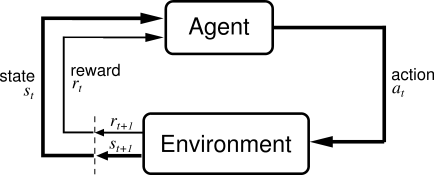
\includegraphics[scale=1]{agent-env-rl}
		\centering
		\caption{Agent-Environment Interface \cite{Sutton-introRL}
			\label{agent-env-rl}}
	\end{figure}
	\subsection{Markov Decision Processes (MDP)} \label{subsec:mdp}
	MDPs are a mathematical framework that facilitates the learning of an optimal mapping between situations(or states) and actions\cite{Sutton-introRL}. A \textit{policy}, referred to by $\pi$ is often the name given to this mapping. Policy learning often occurs through the learning of a \textit{action-value function} or a \textit{state-value function} or both. Formally an MDP is defined by a tuple ${\big\{S,A,P,R, \gamma \big\}}$.
	\begin{itemize}
		\item Here $A$ is a the discrete action space and represents the set of actions that can be performed in the environment and is given by $A = \{a_0,a_1...,a_m\}$. 
		\item $S$ is the state space that represents the set of all possible observable states of the environment and is given by $S = \{s_0,s_1,...,s_n\}$ and $s_t$ is the state at time step $t$. In an MDP all the states are directly observable and can be used to represent the different configurations the environment is in. In non-continuous tasks, such as dialog, each episode ends with a terminal state.
		\item $P$ represents the a function that performs the transition between states. Its job is to return the next state $s_{t+1}$ when we input the presently observed state $s_t$ and the action selected $a_t$ at time $t$. These transitions are modeled by a conditional distribution $P\big(s_{t+1}|s_t,a_t\big)$.
		\item $R$ is the reward function and it returns the immediate reward at time $t$, denoted $r_t$ for the action $a_{t-1} $ and the consequent state transition $s_{t-1} \rightarrow s_t$.
		\item  $\gamma \in \big[0,1\big] $ is called the discount factor that prioritizes short-term rewards.
	\end{itemize}
	At each time step $t$, a particular state $s_t$ characterizes the environment. The agent has to now choose an action $a_t$ according to policy, $\pi : S \rightarrow A$. Due to this interaction with the state, it changes to $s_{t+1}$ according to the transition probabilities and this change could lead to a feedback to the agent as the reward, $r_t = R\big(s_t,a_t,s_{t+1}\big)$. 
	The goal of the agent is to then find a policy which maximizes the expected discounted cumulative reward. Simply, this quantity can be defined as:
	\begin{equation}
	G_t = R_{t+1}+R_{t+2}+R_{t+3}+ \ldots + R_T \label{eq:1}
	\end{equation}
	Where $T$ is the final time-step. To deal with the case of infinite time-steps, we use the concept of \textit{discounting}. Here, the agent tried to select actions so that the sum of the discounted rewards is maximized. The \textit{discount rate}, $0 \leq \gamma \leq 1$ determines the \textit{present value of future rewards}\cite{Sutton-introRL}
	
	\begin{equation}
	G_t = R_{t+1}+\gamma R_{t+2}+\gamma^2 R_{t+3}+ \ldots =  \sum_{k=0}^{\infty} { \gamma ^{k} R_{t+k+1}} \label{eq:2}
	\end{equation}
	Further, (\ref{eq:2}) can be simplified as successive returns are related to each other.
	\begin{align}
	G_t = R_{t+1}+\gamma R_{t+2}+\gamma^2 R_{t+3}+\gamma^3 R_{t+4} \ldots \nonumber\\
	= R_{t+1}+\gamma\big(R_{t+2}+\gamma^2 R_{t+3}+\gamma^3 R_{t+4} \ldots\big) \nonumber\\
	= R_{t+1}+\gamma G_{t+1}  \label{eq:3}
	\end{align}
	Here $G_t$ is expected discounted cumulative reward and $t$ defines the current time-step.
	Now we can define the \textit{value} of a state $s$ given a policy $\pi$ is the total expected return when starting in $s$ and henceforth following $\pi$.
	\begin{equation}
	v_\pi(s) = E_\pi\big[G_t | S_t = s\big] = E_\pi{\bigg[ \sum_{t+1}^{T} { \gamma ^{t+1} R_{t+1} \bigg|S_t = s } \bigg],\ for\ all\ s\in S,} \label{eq:4}
	\end{equation}
	where $E_\pi\big[.\big]$ is the expected value of a given state if the agent follows policy $\pi$ and $t$ is any time-step. $v_\pi$ is known as the \textit{state-value function} for \textit{policy} $\pi$. Likewise, we can define the value of taking an action $a$ in state $s$ given a policy $\pi$, as the expected return starting from $s$, taking action $a$ and thereafter following policy $\pi$:
	\begin{equation}
	q_\pi(s,a) = \mathbb{E}_\pi\big[G_t | S_t = s,\ A_t = a\big] = E_\pi{\bigg[ \sum_{t+1}^{T} { \gamma ^{t+1} R_{t+1} \bigg|S_t = s, \ A_t = a } \bigg]} \label{eq:5}
	\end{equation}
	We call the $q_\pi(s,a)$the  \textit{action-value function} for \textit{policy $\pi$}.
	An important and useful property of value functions used throughout Reinforcement Learning is that they satisfy recursive relationships similar to that of Equation \ref{eq:3}. For any given policy $\pi$ and any state $s$, the following condition holds between the value of $s$ and the value of its possible successor states:
	\begin{align}
	&v_\pi(s) = \mathbb{E}_\pi\big[G_t | S_t = s\big] \nonumber\\
	&= \mathbb{E}_\pi\big[R_{t+1} + \gamma G_{t+1} | S_t = s\big] \nonumber\\
	&=  \sum_{a} { \pi\big(a|s\big)}\sum_{sˆ'}\sum_{r}{p\big(sˆ',r|s,a\big)}\bigg[r+\gamma \mathbb{E}_{\pi}\big[G_{t+1}|S_{t+1} = sˆ'\big]\bigg] \nonumber\\
	&=  \sum_{a} { \pi\big(a|s\big)}\sum_{sˆ',r}{p\big(sˆ',r|s,a\big)}\bigg[r+\gamma v_{\pi}\big(sˆ'\big)\bigg],\text{for all s $\in$ S}  \label{eq:6}
	\end{align}
	Equation \ref{eq:6} is called the \textit{Bellman equation} for $v_{\pi}$. It shows the relationship between the value of a state with respect to the value of its successor states. Similarly the Bellman Equation for $q_{\pi}$ is given by :
	\begin{align}
	q_{\pi}\big(s,a\big) = \sum_{sˆ' \in S}{p\big(sˆ',r|s,a\big)}\bigg(r + \gamma\sum_{aˆ'\in A}\pi\big(s',a'\big)q_{\pi}\big(s',a'\big)\bigg),\\
	\text{for all s $\in$ S and a $\in$ A}\nonumber
	\end{align}
	\subsubsection{Optimality} \label{optimality}
	In essence solving the Reinforcement Learning task aims to find a policy that selects actions in a way that maximizes the future rewards\cite{Sutton-introRL}. In the case of finite MDPs, a policy $\pi$ is said to be better than or equal to a policy $\piˆ'$ if it's expected return is greater than or equal to that of  $\piˆ'$ for all states. So $\pi \geq \piˆ{'}$ if and only if $v_{\pi}(s) \geq v_{\pi^{'}}(s)$ for all $s \in S$. This implies that there is always at least one policy that is better than or equal to all other policies\cite{Sutton-introRL}. This is denoted by $\pi_*$, and it's corresponding state-value function as $v_*$. and is shared by all optimal policies. Thus
	\begin{equation}
	v_*(s) = \max_{\pi} v_{\pi}(s),\ for \ all \ s \in S \label{eq:7}
	\end{equation}
	The \textit{optimal action-value function} is also shared between optimal policies and is denoted by $q_*$
	\begin{equation}
	q_*(s,a) = \max_{\pi} q_{\pi}(s,a),\ for \ all \ s \in S \ and \ a \in A \label{eq:8}
	\end{equation}
	Now for any pair of states and actions, given by $\big(s,a\big)$, equation \ref{eq:8} can give the expected return for taking action $a$ in state $s$ and henceforth following an optimal policy. So from Equations \ref{eq:3},\ref{eq:4} and \ref{eq:5}, we can define $q_*$ in terms of $v_*$,
	\begin{equation}
	q_*(s,a) = E\big[R_{t+1} + \gamma v_* \big(S_{t+1}\big)| S_t = s,A_t = a ] \label{eq:9}
	\end{equation}
	Now since $v_*$ is the value function for a policy it must satisfy the condition given by Equation \ref{eq:6}. But, since it tis the optimal value function, it can be defined without reference to any specific policy. This is known as the Bellman Equation for $v_*$ or the \textit{Bellman optimality equation}. Intuitively, it can be seen that when working with an optimal policy the return for the optimal action in that state must be the same as the value of that state.\cite{Sutton-introRL}
	\begin{align}
	&v_*(s) = \max_{a \in A\big(s\big)} q_{\pi_*}(s,a) \nonumber\\
	&= \max_{a} \mathbb{E}_{\pi_*} \big[ G_{t} | S_t = s, A_t = a\big] \nonumber\\
	&= \max_{a} \mathbb{E}_{\pi_*} \big [R_{t+1} + \gamma G_{t+1}  | S_t = s, A_t = a\big] \nonumber\\
	& = \max_{a} \mathbb{E} \big [R_{t+1} + \gamma v_{*}\big(S_{t+1}\big)  | S_t = s, A_t = a\big] \nonumber\\
	& = \max_{a} \mathbb{E} \big [R_{t+1} + \gamma v_{*}\big(S_{t+1}\big)  | S_t = s, A_t = a\big] \nonumber\\
	&= \sum_{sˆ',r}{p\big(sˆ',r|s,a\big)}\bigg[r+\gamma v_{*}\big(sˆ'\big)\bigg] \label{eq:10}
	\end{align}
	The Bellman Optimality Equation for $q_*$ is given by,
	\begin{align}
	&q_*\big(s,a\big) =  \mathbb{E} \big [R_{t+1} + \gamma \max_{aˆ'} q_{*}\big(S_{t+1},a\big)  | S_t = s, A_t = a\big] \nonumber\\
	&= \sum_{sˆ',r}{p\big(sˆ',r|s,a\big)}\bigg[r+\gamma \max_{aˆ'} q_{*}\big(sˆ',aˆ'\big)\bigg] \label{eq:11}
	\end{align}
	Equations \ref{eq:10} and \ref{eq:11} are the Bellman Optimality Equations for $v_*$ and $q_*$ respectively.
	
	\subsection{Composing Dialog Management as an MDP}\label{dialog-mdp}
	Dialog Management (DM) \cite{Young99probabilisticmethods} is the primary task of any dialog system. The job of the dialog manager is to predict best system action or utterance to the user provided information such as the user utterance, dialog history ,knowledge of possible systems actions and other domain-specific information or features. Collective this can be called the dialog context. Thus the DM has to take the best actions i.e. make good \textit{decisions} based on often times incomplete and highly variant \textit{contexts} in order to eventually achieve a \textit{reward}. This learning of an optimal mapping between situations and actions otherwise is called a \textit{policy}. This definition of the problem allows us to cast dialog management as a sequential decision making problem. First done by Pieraccini et. al \cite{mdp-pieraccini} who cast the DM problem as a Markov Decision Process (MDP) \cite{mdp-bellmann}. Since the MDP framework comes from optimal control theory we mainly consider the decision making process as a \textit{control} problem. To start of, some probabilistic description of the problem use case is made which requires knowledge of some of its parameters. If some of these parameters are unknown the Reinforcement Learning(RL) paradigm \cite{Sutton-introRL} provides approximate solutions for optimization of policies. In this context the DM is seen as an agent which has to interact with its environment (the human user) to maximize some expected reward. This reward is ideally returned only when the user is satisfied or a domain related goal is reached.
	\begin{figure}[H]
		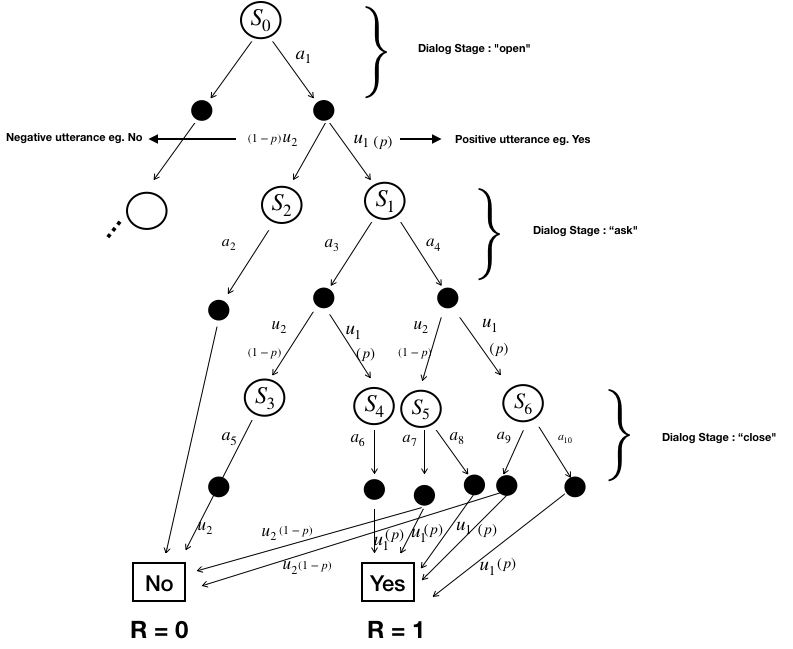
\includegraphics[scale=0.65]{user-env4-2}
		\centering
		\caption{Dialog represented as a Markov Decision Process
			\label{chat-world3}}
	\end{figure}
	Reinforcement Learning(RL) can be applied in a fairly straightforward manner to conversational models casted as MDPs. The Reinforcement Learning Agent's(RLA) Policy, observes a discrete state at time step $t$ represented by the current position of the dialog in the dialog MDP shown in Figure \ref{chat-world3}. Thus the current  state represents the sequence or path given by the arcs between all previous user input utterances, dialog states and system actions. The Dialog MDP otherwise called the \textit{conversation graph} is given by nodes that represent the actions/utterances from the RL Agent or utterances that the user or environment inputs. When the edges originate from a dialog state such as \{$S_0,S_1...$\} of the RL Agent, they represent the agents actions such as \{$a_0,a_1...$\}. When the edges originate from the hidden user states they are utterances that the user inputs, represented by \{$u_0, u_1...$\}. Thus each observable state of the Agent is a function of the history of the dialog and the previous user utterance. This state is also called the \textit{dialog state}. This modeling of the dialog state is based on the \textit{Information State Paradigm}\cite{Larsson:2000:ISD:973935.973943}, where the dialog environment is modeled as a discrete state space with a unique state number for each state otherwise known as finite state models. Our dialog system is task-oriented with the objective being the successful conversion of a service call to sell a product. Here the the objective can be summarized as making the best actions for a given dialog state to increase the chances of getting a positive response from the user.\par
	\begin{figure}[H]
		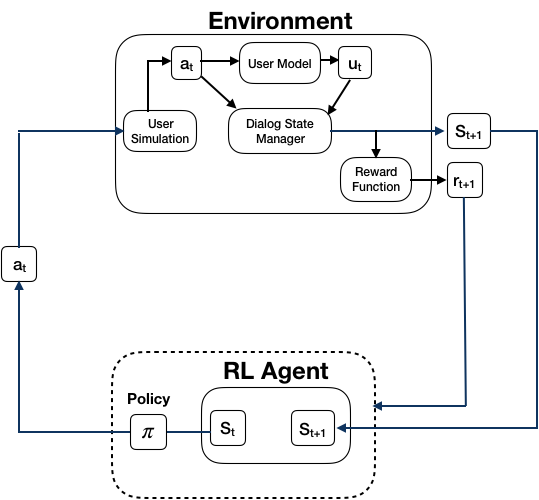
\includegraphics[scale=0.65]{user-env}
		\centering
		\caption{Agent-Environment Interaction
			\label{chat-world}}
	\end{figure}
	To carry out a Dialog, the Agent may greet the user and recommend a product and opening question for their customer. If this receives a positive response, the agent suggests a follow up question that leads to a sale, if this is positive then the system closes the sale. These acts or dialog moves form the action set. With regard to real users the transition probabilities are unknown but can be sampled by letting the user interact with the agent. However, for reasons of practicality, we first train the agent on simulated users created with transition probabilities according to broad categories of demographic data of actual users. For both real and Simulated users a reward is given to the  agent upon successfully selling a product to a customer i.e. If the customer shows interests, which means in the model that certain affirmative terminal states are reached, a reward is generated, e. g. $R = 1$. In conversation with variable length we can consider to penalize the agent by assigning a small negative reward to every round, e. g. $ R = -0.1$. The interaction between the Reinforcement Learning Agent (RL Agent) and the Environment, which includes the Simulated User is shown in Figure \ref{chat-world}.
	\begin{figure}[H]
		\vspace{0.2cm}
		\centering
		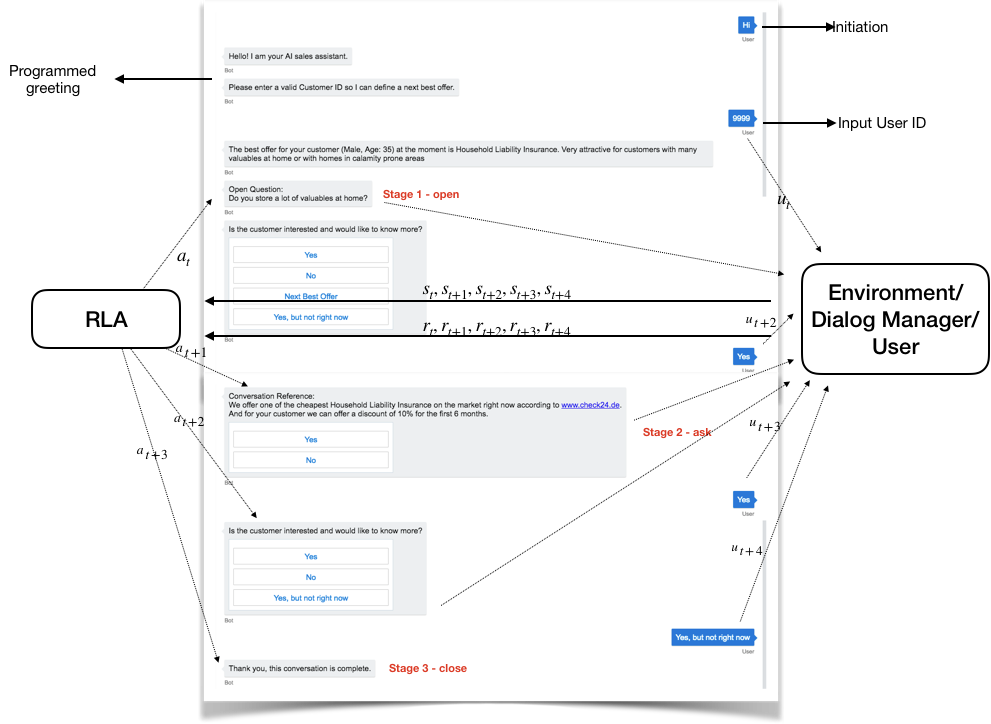
\includegraphics[scale=0.5]{user-env3}
		\caption{Agent-Environment Interaction in the form of a chatbot application
			\label{chat-world2}}
	\end{figure}
	Here $S_t$ and $S_{t+1}$ represents the current and next observable state of the environment. $a_t$ is the currently chosen action from the policy $\pi$ approximated by the Reinforcement Learning Agent(RLA). $u_t$ represents the utterance/response from a simulated user to the current action(statement/question) $a_t$ from the RLA. This utterance $u_t$ along with the current action $a_t$ is fed into the Dialog State Manager(DSM) which manages the next state of the environment. The DSM then consults the reward function, which generates the reward(if any) for the current state. The Reward and the new State are then given to the RLA, which takes the new state as the current state and repeats the process. This process is expressed more clearly in the view of the chat-bot implementation in Figure \ref{chat-world2}. Here we see the User Input Utterance (In Blue) as well as the the most recent action from the agent is fed to the environment which then returns the next state and the reward for the current step to the Agent.
	\subsection{Dialog Policy Optimization}
	\begin{figure}[H]
		\centering
		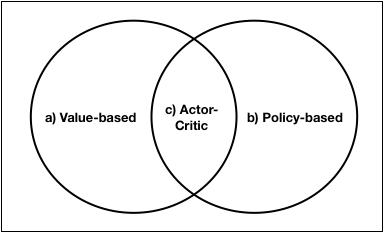
\includegraphics[scale=0.7]{mdp_methods}
		\caption{Dialog Policy Optimization Methods
			\label{mdp-methods}}
	\end{figure}
	The RL paradigm offers us many varieties and flavors of algorithms\cite{rl_overview} to help us optimize policies and to consequently solve MDPs. Generally these can be broadly categorized as methods that :
	\begin{itemize}
		\item Iteratively improve a value function which help find a good policy by learning better state or action values. Known as Value-Based Methods.
		\item Directly parametrize the policy and iteratively improve it without using any value function. Known as Policy-Based Methods
		\item Iteratively improve both value function and policy. Known as Actor-Critic Methods
	\end{itemize}
	These methods are discussed in further below. In this work, we assume our dialogs to be episodic and thus considered to have a finite number of steps T. In order to find the best policy we must train our policy $\pi$ to maximize the discounted cumulative reward per episode. Thus considering Equation \ref{eq:2} with final time step as $T$ and current time step as $t$, we get,
	\begin{equation}
	R_t =\sum_{t}^{T} { \gamma ^{t} R_{t+1}}, \text{while following policy $\pi$ } \nonumber
	\end{equation}
	This is the value that has to be maximized and we first see how to do this by improving the value function.
	\subsubsection{Value Iterative Methods}
	As we have seen in Section \ref{optimality}, one can represent the expected cumulative reward at a state $s$ following a specific policy $\pi$ by using a state-value function, which is a semantic mapping between the state and the expected cumulative reward i.e. 
	$V: s \rightarrow R$, this is represented by Equation \ref{eq:4}. Similarly we have the action-value function which is semantically a mapping between state, action pairs and total expected cumulative reward i.e. $Q: \big(S,A\big) \rightarrow R$, this is represented by Equation \ref{eq:5}. Now Equations \ref{eq:4} and \ref{eq:5} together with \textit{Bellman's Optimality Condition} \ref{eq:7} \cite{Sutton-introRL}, gives us the Optimal state-value function, represented by Equation \ref{eq:10}, and the optimal action-value function, represented by Equation \ref{eq:11}. Finally, if $q_*\big(s,a\big)$ is the optimal action-value function for a policy $\pi$, this implies that the optimal policy $\pi_*$ behavior is controlled by
	\begin{equation}
	\pi_*\big(s\big) = arg \max_{a} q_*\big(s,a\big) \label{eq:12}
	\end{equation}
	And in the above Equation if we substitute the value of $q_*\big(s,a\big)$ with Equation \ref{eq:10}, we get 
	\begin{equation}
	\pi_*\big(s\big) = arg \max_{a} \sum_{sˆ',r}{p\big(sˆ',r|s,a\big)}\bigg[r+\gamma v_{*}\big(sˆ'\big)\bigg] \label{eq:13}
	\end{equation}
	Thus we can see from Equations \ref{eq:12} and \ref{eq:13} that we can arrive at the optimal policy $\pi_*$ by selecting actions that maximize the state-value function or the action-value function (Q-function). In the perspective of dialog systems this would imply that by selecting the system responses that maximizes cumulative reward for every conceivable dialog state and consequently follow a dialog policy $\pi$, we can iteratively arrive at the best possible policy $\pi_*$ that represents the best sequence of responses.
	\myparagraph{Dynamic Programming}\label{dp}
	These techniques primarily depend on using the value functions given by Bellman Optimality Equations  \ref{eq:10} and \ref{eq:11}. Dynamic programming is a process of solving MDP's i.e.\ finding the optimal value function, given by Equations \ref{eq:7} and \ref{eq:8}. This is achieved by recursively computing the value os states and/or actions using some known model of the MDP with the Bellman Optimality Equation as an update rule. This process is also known as basic value iteration and the value of a state-action pair can be recursively updated by the rule \cite{Sutton-introRL} :
	\begin{align}
	q_{t+1}\big(s,a\big) = \sum_{s,s' \in S} p\big(s',r | s,a \big)[r + \gamma \max_{aˆ'}q_t\big(s',a'\big)] \label{eq:dp-update}
	\end{align}
	Another common DP method is known as policy iteration here we first evaluate the value of a specific policy $\pi$ using Equation \ref{eq:13}. From this value computation, a policy improvement step is performed that creates a new policy by behaving \textit{greedily} with respect to this new learned value. This recursive process repeats until the optimal policy or a policy very close to it is found\cite{Sutton-introRL}.
	Policy iterations, thus consists of two interacting processes, one that updates the value making it match the current policy(evaluation) and the other taking greedy policy actions with respect to the learned value(improvement). Generally these processes alternate with one completing before the other starts. Generalized Policy Iteration(GPI) is the process of letting policy evaluation and improvement interact independent of the other details of these processes\cite{Sutton-introRL} i.e.\ in GPI the change between evaluation and improvement is made before the current process is complete.
	\myparagraph{Monte Carlo Learning }\label{mc-learning}
	These methods play upon the ideas of GPI. As we know GPI consists of twi steps, policy evaluation and improvement. In MC techniques the value is estimated by completely rolling out the current policy on the system i.e.\ executing the policy based actions step by step across a full episode of learning. This process accumulates the reward returned over the entire episode with respect to the various states that the system encountered on the way, which is then used to compute the value function. This is followed by usual policy improvement by acting greedy with respect to current value function and generating a new better policy. Following these two steps repeatedly can be shown to converge to the optimal policy and value function. Though these methods are straightforward to understand and implement, in practice they require a very large number of iterations to converge and further show a high amount of variance in the estimated values.
	\myparagraph{Temporal Difference(TD) Learning }\label{td-learning}
	The combination of the above approaches of Monte Carlo and Dynamic Programming give us TD learning. Since its invention in the 1980's by Richard Sutton \cite{sutton1988TFDearning} it has come to be a central idea in RL. Typically in TD learning like DP, the computed estimates are updated with respect to other learned estimates but without waiting for any one process to converge before starting the other. An important concept here is the TD error $\delta$. $\delta$ is defined as the error or discrepancy between the expected return and the currently  received return and thus can be represented as the update:
	\begin{align}\label{eq:td-error}
	\delta_{t} = r_{t+1} + \gamma v\big(s_{t+1}\big) - v\big(s_t\big) 
	\end{align}
	This the TD error ae any time $t$ is discrepancy found in the value estimate at that time. Since this error depends on the following state and reward, $\delta_{t}$ is not available until time $t+1$. According to Sutton's TD algorithm that incorporates policy iteration, the value function for a policy can be estimated by incrementally following the update\cite{sutton1988TFDearning} :
	\begin{align}\label{eq:td-update}
	v \big(s_t\big) = v\big(s_t\big) + \alpha_t\delta_{t+1}
	\end{align}
	Where $\alpha_t \in (0,1] $ is the learning rate at the time $t$ and is designed to be weighting that sets the importance of considering the old and new estimate of the value function. 
	The learning rate controls the convergence properties of the update process describes in Equation \ref{eq:td-update} as the update process convergence only when the learning rate satisfies what is known as the \textit{Robbins-Monro} convergence theorems. This is given by :
	\begin{enumerate}
		\item $\sum_{t=0}^{\infty}\alpha_t = \infty$
		\item $\sum_{t=0}^{\infty}\alpha_t^2 < +\infty$
		\item $\alpha_t \geq 0, \forall t$
	\end{enumerate}
	from this it also follows that all state-action pairs would be been visited nearly infinitely many times before convergence. These principle have been applied for decades in RL with huge success. The most well known algorithms that emerge from this framework are \textit{Q-learning} and \textit{Sarsa}. 
	Sarsa works \textit{on-policy} which means that it works iteratively to estimate the action-value function of the currently followed policy by following the update:
	\begin{align}\label{eq:sarsa-update}
	q\big(s_t,a_t\big) = q\big(s_t,a_t\big) + \alpha_t\big[r_t + \gamma q\big(s_{t+1},a_{t+1}\big) - q\big(s_t,a_t\big)\big]
	\end{align}
	Thus the policy evaluation step uses the TD error for computing the action-value, the complete algorithm can be found below.
	\begin{algorithm}[h]
		\DontPrintSemicolon
		\SetAlgoLined
		\SetKwInOut{Parameter}{Initialize}
		\SetKwInOut{Input}{Input}\SetKwInOut{Output}{Output}
		\Parameter{$q(s,a)$ randomly for all $s \in S$ and $a \in A(s)$}
		\Repeat{terminated}{
			Observe initial state $s_1$\;
			Choose action $a_1$ using policy derived from $Q$ (by $\epsilon$-greedy behavior)\;
			\For{t = 1,...,T}{
				Take action $a_t$\;
				Observe reward $r_t$ and new state $s_{t+1}$\;
				Choose next action $a_{t+1}$ using policy derived from $Q$ (by $\epsilon$-greedy behavoir)\; 				
				Update Q function by $q\big(s_t,a_t\big) = q\big(s_t,a_t\big) + \alpha_t\big[r_{t+1} + \gamma q\big(s_{t+1},a_{t+1}\big) - q\big(s_t,a_t\big)\big]$\;
				$s_t \gets s_{t+1}$\;
				$a_t \gets a_{t+1}$\;
			}
		}
		
		\caption{SARSA}\label{alg:sarsa}
	\end{algorithm}
	\textit{Off-policy} methods are complimentary to the above in the sense that these methods attempt to learn a value function for a policy that differs from the policy that was used to choose the current actions, i.e.\ the target policy differs from current used policy. Watkin's in 1989 invented the famous Q-learning algorithm\cite{watkins1989Qlearning}. This algorithm is similar to Sarsa but works off-policy and uses a different update rule. Here the update rule is defined as 
	\begin{align}\label{eq:q-update}
	q\big(s_t,a_t\big) = q\big(s_t,a_t\big) + \alpha_t\big[r_t + \gamma \max_{a}q\big(s_{t+1},a_t\big) - q\big(s_t,a_t\big)\big]
	\end{align}
	The complete Q-learning Algorithm can be found below:
	\begin{algorithm}[h]
		\DontPrintSemicolon
		\SetAlgoLined
		\SetKwInOut{Parameter}{Initialize}
		\SetKwInOut{Input}{Input}\SetKwInOut{Output}{Output}
		\Parameter{$q(s,a)$ randomly for all $s \in S$ and $a \in A(s)$}
		\Repeat{terminated}{
			Observe initial state $s_1$\;
			
			\For{t = 1,...,T}{
				Choose action $a_t$ using policy derived from $Q$ (by $\epsilon$-greedy behavior)\;
				Take action $a_t$\;
				Observe reward $r_t$ and new state $s_{t+1}$\;		
				Update Q function by $q\big(s_t,a_t\big) = q\big(s_t,a_t\big) + \alpha_t\big[r_t + \gamma \max_{a}q\big(s_{t+1},a_t\big) - q\big(s_t,a_t\big)\big]$\;
				$s_t \gets s_{t+1}$\;
			}
		}
		
		\caption{Q-Learning}\label{alg:q-learning}
	\end{algorithm}
	\myparagraph{Sample Efficiency}
	All the TD techniques we saw above works by individually using each same a single time for updating the value. It is found that this learning can be accelerated by using multiple samples efficiently. A common way to achieve this is by using \textit{Eligibility Traces}, here the trace $e \colon S \times A \rightarrow [0,\infty)$ propagates the current reward $r_t$ to update the values of recently encountered states. The update rule of the above algorithms with eligibility traces become:
	\begin{align}
	q\big(s_t,a_t\big) = q\big(s_t,a_t\big) + \alpha_t\delta_{t}e_t, \forall s,a \ \text{and} \ e_0 = 0
	\end{align}
	Here every state has an additional variable associated to it known as its trace, $e_t(s,a) \in \mathbb{R}$. This trace represents the discrepancy in the value of each state-action pair at every time step and is dependent on the number of individual encounters with that state was followed by taking that action. These traces are updated at each time step using the update rule:
	\begin{align}
	e_t(s,a) = \begin{cases}
	\lambda\gamma e_{t-1}\big(s,a\big) & \text{if }\big(s,a\big) \neq \big(s_t,a_t\big) \\    
	1 & \text{if }\big(s,a\big) = \big(s_t,a_t\big)
	\end{cases}
	\end{align}
	Where $\lambda$ is called the \textit{trace-decay}.
	Another important method which enables faster learning and greater sample efficiency is by recording the transition history e.g.\ $(s_t,a_t,s_{t+1},a_{t+1}...)$ and using them at the ends of each episode to update the value, thus replaying the transitions in the update rule. This is known as \textit{Experience Replay} and has been shown to be very successful in accelerating learning\cite{adam2012experience}.
	
	\myparagraph{Function Approximation} \label{fn_aprrox}
	In the previous section we just discussed how we could find the optimal state-value or action-value function and thus the optimal policy by iteratively selecting actions that maximize our estimate of these functions.  The methods described above generally estimate the value functions using some static data structure such as a look-up table. This generally functions well when the environment and domain has a small and manageable state or state-action space.  When this space is very large of the order $10^5$ or greater, then this solution becomes very slow and intractable due to the large number dimensions, this is commonly known as the curse of dimensionality\cite{verleysen2005curse}. A good solution is to employ function approximation techniques that substitutes the above mentioned look-up table with a representation such as a decision tree, linear functions or most popularly, neural networks. Neural Networks are known be excellent Universal Function Approximators \cite{hornik1989multilayer} which means they can model any continuous function. Modeling our value functions as neural networks is advantageous in very large and continuous state-action spaces as it makes the solution tractable and we can represent the function as a linear combination of features which represent different portions of the large state space. This lets us generalize well from observed to unobserved states as any update to the parameters will also update the value function which affects the \textit{value} of all states. Thus we can represent the complex and large state space as a set of features $\{f_1,f_2,...,f_n\}$, here $n$ is the number of features. Now if we consider our actions as a factored set of state-oriented allowed actions we can represent the action-value function (and any Utility function in general) as: 
	\begin{equation}
	Q^a\big(s,a\big) = {\theta_1^a}f_1+\dots+{\theta_n^a}f_n
	\end{equation}		
	Where $a$ is each action and $\theta = \{\theta_1,...,\theta_n\}$ are the parameters of the neural network. Now a RL agent can learn the values of $\theta$ to approximate the value-function. 
	
	\subsubsection{Policy Iterative Methods}\label{policy_methods}
	Previously we saw how a value function could represent the most optimal policy $\pi_*$. Another solution to finding the optimal policy is to directly parametrize the policy $\pi$ itself. These techniques aim at iteratively optimizing the policy directly. Here we work in the policy space and not in the state-action space like before. A function parameterized with respect to $\theta$  is chosen to represent 
	the policy $\pi_{\theta}\big(a|s\big)$. The reward function to be maximized depends on this policy and is given by: 
	\begin{equation}
	J\big(\theta\big) = \sum_{s \in S} d_{\pi}\big(s\big)v_{\pi}\big(s\big) =\sum_{s \in S} d_{\pi}\big(s\big) \sum_{a \in A} \pi_{\theta}\big(a|s\big)q_{\pi}\big(s,a\big)
	\end{equation}
	Now consider traveling along a Markov Process's states forever, once all states are explored and seen multiple times, eventually, the probability of assuming any single state becomes stable and unchanged - this is called the \textit{Stationary Probability} for $\pi_{\theta}$ and is represented by $d_{\pi}$. Now to improve the objective function we need to compute its gradient, $\nabla J\big(\theta\big) $
	The Policy Gradient Theorem now gives us an expression an expression for the gradient of the objective function states that for the Objective Function $J\big(\theta\big)$, generally this is a problem as it is dependent on the action-selection behavior and the state-wise stationary distribution we spoke about earlier. Generally since the environment is unknown, this computation is intractable. Here is where the Policy Gradient Theorem comes in and gives us an expression for the gradient that \textit{does not} depend on the derivative of the distribution $d_{\pi}\big(s\big)$. Thus the PG theorem shows that :
	\begin{equation}
	\nabla J\big(\theta\big) \propto \sum_{s \in S} d_{\pi}\big(s\big) \sum_{a \in A}q_{\pi}\big(s,a\big) \nabla \pi\big(a|s,\theta\big)
	\end{equation}
	
	To arrive at this relation, we follow the conventions in \cite{Sutton-introRL} and start by considering the partial derivative of the state-value function $v_\pi\big(s\big)$:
	\begin{align}
	&\nabla_{\theta} v_\pi\big(s\big) = \nabla_{\theta} \bigg(\sum_{a \in A} \pi_{\theta}\big(a|s\big)q_\pi\big(s,a\big)\bigg), &&\text{From Eq. \ref{eq:6}}\nonumber\\
	&=\sum_{a \in A}\bigg(\nabla_{\theta}\pi_{\theta}\big(a|s\big)q_\pi\big(s,a\big)+\pi_{\theta}\big(a|s\big)\nabla_{\theta}q_\pi\big(s,a\big)\bigg),\nonumber\\
	&\text{Using the product rule},\nonumber\\
	&=\sum_{a \in A}\bigg(\nabla_{\theta}\pi_{\theta}\big(a|s\big)q_\pi\big(s,a\big)+\pi_{\theta}\big(a|s\big)\nabla_{\theta}\sum_{sˆ',r}{p\big(sˆ',r|s,a\big)}\bigg[r+\gamma v_{\pi}\big(sˆ'\big)\bigg]\bigg),&&\text{From Eq. \ref{eq:10}}\nonumber\\
	&\text{Now to simplify we consider $\gamma = 1$ and since $r$ does not depend}\nonumber\\
	&\text{on $\theta$ we can eliminate it. Also we know that:}\nonumber\\
	&P\big(sˆ'|s,a\big) = \sum_{r} P\big(sˆ',r|s,a\big) \nonumber\\
	&\text{This lets us simplify the above as}\nonumber\\
	&\nabla_{\theta} v_\pi\big(s\big)=\sum_{a \in A}\bigg(\nabla_{\theta}\pi_{\theta}\big(a|s\big)q_\pi\big(s,a\big)+\pi_{\theta}\big(a|s\big)\sum_{sˆ'}{p\big(sˆ'|s,a\big)}\nabla_{\theta} v_{\pi}\big(sˆ'\big)\bigg)  \label{eq:17}
	\end{align}
	Now if we notice the term on the LHS and the final term in the RHS, we can see that the above Equation \ref{eq:17} is recursive. This means that we can \textit{role out} the final term to
	\begin{align}
	&\nabla_{\theta} v_\pi\big(s\big)=\sum_{a \in A}\bigg(\nabla_{\theta}\pi_{\theta}\big(a|s\big)q_\pi\big(s,a\big)+\pi_{\theta}\big(a|s\big)\sum_{sˆ'}{p\big(sˆ'|s,a\big)}\nonumber\\
	&\sum_{aˆ'\in A}\bigg[\nabla_{\theta}\pi_{\theta}\big(aˆ'|sˆ'\big)q_\pi\big(sˆ',aˆ'\big)+\pi_{\theta}\big(aˆ'|sˆ'\big)\sum_{sˆ''}p\big(sˆ''|sˆ',aˆ'\big)\nabla_{\theta} v_{\pi}\big(sˆ''\big)\bigg]\bigg)   &&\text{From Eq. \ref{eq:17}}\nonumber\\
	\end{align}
	Now to simplify this recursive equation we generalize the probability of moving from any state $s$ to any other state $x$ in $k$ steps while following policy $\pi_{\theta}$ as $Pr\big(s\rightarrow x, k, \pi_{\theta}\big)$. This lets us rewrite the above equation in a generalized form as
	\begin{align}
	&\nabla_{\theta} v_\pi\big(s\big)= \sum_{x \in S} \sum_{k=0}^{\infty} Pr\big(s\rightarrow x, k, \pi_{\theta}\big) \sum_{a \in A}\nabla_{\theta}\pi_{\theta}\big(a|x\big)q_{\pi}\big(x,a\big)
	\end{align}
	Finally this generalized equation lets us exclude the derivative of the action value function $\nabla_{\theta}q_{\pi}\big(s,a\big)$ by plugging it back into the objective function $J\big(\theta\big)$. Considering that we start from any random state $s_0$ we get:
	\begin{align}
	&\nabla_{\theta}J\big(\theta\big) = \nabla_{\theta}v_{\pi}\big(s_0\big)\nonumber\\
	& = \sum_{s} \bigg(\sum_{k=0}^{\infty}Pr\big(s_0\rightarrow s, k, \pi_{\theta}\big)\bigg)\sum_{a}\nabla_{\theta}\pi_{\theta}\big(a|s\big)q_{\pi}\big(s,a\big) \label{eq:obj_value}
	\end{align}		
	Let $\eta\big(s\big) = \sum_{k=0}^{\infty}Pr\big(s_0\rightarrow s, k, \pi_{\theta}\big)$. Now we get
	\begin{align}
	&\nabla_{\theta}J\big(\theta\big)= \sum_{s}\eta\big(s\big)\sum_{a}\nabla_{\theta} \pi_{\theta}\big(a|s\big)a_{\pi}\big(s,a\big)\nonumber\\
	& = \bigg(\sum_{s}\eta\big(s\big)\bigg)\sum_{s}\frac{\eta\big(s\big)}{\sum_{s}\eta\big(s\big)}\sum_{a}\nabla_{\theta} \pi_{\theta}\big(a|s\big)q_{\pi}\big(s,a\big)&&\text{by normalizing $\eta\big(s\big)$} \nonumber
	\end{align}		
	Now since $\sum_{s}\eta\big(s\big)$ is a constant and considering $ d_{\pi}\big(s\big) = \frac{\eta\big(s\big)}{\sum_{s}\eta\big(s\big)}$, we get:
	\begin{align}
	&\nabla_{\theta}J\big(\theta\big)\propto \sum_{s}d_{\pi}\big(s\big)\sum_{a}\nabla_{\theta} \pi_{\theta}\big(a|s\big)q_{\pi}\big(s,a\big)
	\end{align}
	This is known as the Policy Gradient Theorem \cite{Sutton-introRL}\cite{Sutton_pg}.
	Now if we consider the \textit{episodic} case, where each episode of training has a distinct starting and terminal state, the proportionality constant $\sum_{s}\eta\big(s\big)$ is defined as the average length of an episode. Thus the gradient can be further simplified as:
	\begin{align}
	&\nabla_{\theta}J\big(\theta\big)\propto \sum_{s}d_{\pi}\big(s\big)\sum_{a}q_{\pi}\big(s,a\big)\nabla_{\theta} \pi_{\theta}\big(a|s\big)\nonumber\\
	& = \sum_{s}d_{\pi}\big(s\big) \sum_{a} \pi_{\theta}\big(a|s\big) q_{\pi}\big(s,a\big) \frac{\nabla_{\theta}\pi_{\theta}\big(a|s\big)}{\pi_{\theta}\big(a|s\big)}\nonumber\\
	& = \mathbb{E}_{\pi}\big[q_{\pi}\big(s,a\big)\nabla_{\theta}\ln\pi_{\theta}\big(a|s\big)\big]\label{eq:vpg_update}
	\end{align}
	This is known as the \textit{Vanilla} Policy Gradient update and lays the theoretical foundation foundation for the various policy gradient algorithms found in Section \ref{dm-with-drl}
	\subsubsection{Actor-Critic Methods}\label{section:ac-methods}
	In this chapter we will introduce and derive the Actor-Critic framework. These methods are known for combining both the techniques we saw above i.e.\ Value based optimization which is known as the Critic as intuitively it \textit{judges} the quality of the action or \textit{act} chosen by the actor Policy. The complete functioning of this process can be seen in Figure \ref{a-c}. 
	\begin{figure}[h]
		\centering
		\setlength{\fboxsep}{5pt}%
		\setlength{\fboxrule}{1pt}%
		\fbox{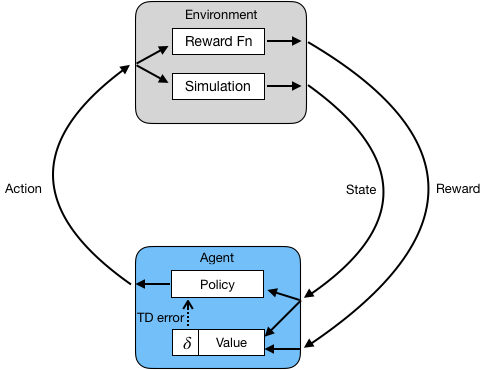
\includegraphics[scale=0.6]{a-c}}
		\caption{Actor-Critic Environment Interaction
			\label{a-c}}
	\end{figure}
	In the previous section we saw the PG theorem\cite{Sutton-introRL}\cite{Sutton_pg} which helped us estimate the gradient of the objection function for a parameterized policy i.e.\ the \textit{policy gradient}. According to this, the policy gradient for any MDP is given by:
	\begin{align}
	&\nabla_{\theta}J\big(\theta\big) =  \sum_{s}d_{\pi}\big(s\big)\sum_{a}\nabla_{\theta} \pi_{\theta}\big(a|s\big)q_{\pi}\big(s,a\big) \label{eq:pg-theorem}
	\end{align}
	Here a great advantage is that there is no gradient of the steady state distribution as discussed in the previous section. This means that if we obtain training samples by following a policy $\pi_{\theta}$, then $\sum_{a}\nabla_{\theta} \pi_{\theta}\big(a|s\big)q_{\pi}\big(s,a\big)$  represents an unbiased estimate of $\nabla_{\theta}J\big(\theta\big)$ and also a gives us a relation between the policy gradient and value function or critic. 
	The PG theorem also lets us parameterize the value function. Consider $f_w(s,a) \colon S \times A \rightarrow R$ as an approximation of the value function $q_{\pi}(s,a)$ where $w$ represents the weights of parameterization. Generally since function approximators such as neural networks try to minimize the discrepancy between the true value function $q_{\pi}(s,a)$ and its approximation $f_w(s,a)$, we get an update rule for $w$ which is of the form $\nabla w \propto \nabla_w[q_{\pi}(s,a) - f_w(s,a)]\propto [q_{\pi}(s,a) - f_w(s,a)]\nabla_w[f_w(s,a)]$. Using this in Equation \ref{eq:pg-theorem} we get convergence if we successfully approximate $q_{\pi}(s,a)$  as:
	\begin{align} &\sum_{s}d_{\pi}\big(s\big)\sum_{a} \pi_{\theta}\big(a|s\big) [q_{\pi}(s,a) - f_w(s,a)]\nabla_w[f_w(s,a)] = 0 \label{eq:ac-conv}
	\end{align}
	Now when $f_w(s,a)$ satisfies the above, we get the following relation from Equation \ref{eq:vpg_update} :
	\begin{align}
	\nabla_w[f_w(s,a)] = \nabla_{\theta}[\ln\pi_{\theta}\big(a|s\big)] \label{eq:pg-compatible}
	\end{align}
	Now by plugging in the RHS of Equation \ref{eq:pg-compatible} into Equation \ref{eq:ac-conv} we get:
	\begin{align} &\sum_{s}d_{\pi}\big(s\big)\sum_{a} \nabla_{\theta}\pi_{\theta}\big(a|s\big) [q_{\pi}(s,a) - f_w(s,a)] = 0 \label{eq:ac-error}
	\end{align}
	Thus we can see that the error in approximating the value function is perpendicular to the policy gradient. Since the above equation is equal to 0, we can subtract Equation \ref{eq:ac-error} from Equation \ref{eq:pg-theorem} which gives :
	\begin{align}
	&\nabla_{\theta}J\big(\theta\big) =  \sum_{s}d_{\pi}\big(s\big)\sum_{a}\nabla_{\theta} \pi_{\theta}\big(a|s\big)f_w\big(s,a\big) \label{eq:pg-f}
	\end{align}
	Thus when the value approximation satisfies Equation \ref{eq:ac-conv} and \ref{eq:pg-compatible}, we get a reliable estimate of the policy gradient from Equation \ref{eq:pg-f}. Now since $f_w$ has 0 mean for any particular state i.e.\ invariant to state or action distribution, we have:
	\begin{align}
	\sum_{a} \pi_{\theta}\big(a|s\big)f_w\big(s,a\big) = 0, &&\forall s\in S
	\end{align}
	By this we can think of $f_w$ as some \textit{advantage function}: $A_{\pi}(s,a) = q_{\pi}(s,a) - v_{\pi}(s)$ \cite{peters2005natural}\cite{Sutton_pg}. Thus we can introduce what is known as a baseline function $b\colon S \rightarrow R$\cite{peters2005natural} without changing the results of Equation \ref{eq:pg-f}. This baseline $b(s)$ can have a great influence on the performance of the gradient approximators \cite{Sutton_pg}. Now if we have a parameterized baseline $b_{w_2}$ with parameter $w_2$ and a parameterized value approximation $f_{w_1}$ with parameters $w_1$ we can get the value function approximation $q_w$ as:
	\begin{align}
	q_w = f_{w_1}\big(s,a\big) + b_{w_2}\big(s\big)
	\end{align}
	where $w = [w_1^T w_2^T]^T$. We will further explore this method in Section \ref{a2c-section} but an important property here is that t he convergence to some policy is guaranteed given that the value function approximate follows the above conditions.
	\subsection{Evaluation and Reward Estimation}
	Typically evaluating large dialog systems is known to be a complex and difficult task. Primarily, this is due to the long term interactions and history between the dialog system and the human user. The fact that a typical large scale dialog system includes sub components such as a NLU and NLG, make things even more complicated and even though these systems can be individually evaluated, the joint evaluation of the entire system is still considered to be very difficult. The easiest and most intuitive method of evaluating a dialog system is also generally the most expensive, that is using real human interaction to judge the dialog, but this too is susceptible to human generated subjective biases. In cases where we develop end-to-end open-domain dialog systems with a corpus of dialogs that the systems needs to learn to mimic, certain similarity metrics such as \textit{word-overlap} can be used\cite{bordes2016learning}, but this too in known to be highly variant when compared to human evaluation of the same systems\cite{liu2016not}. Since in this work we deal with task-oriented dialog, we can use task-completion as a straightforward and automatic measurement that makes sure the learning strategy is valid. When applying RL techniques to develop dialog systems these task-completion signals can be used as a high-level objective during learning, this is also known as the \textit{reward} in colloquial RL terminology.
	\subsubsection{Heuristic Rewards}
	The reward signal plays a major role in the MDP framework as it directly defines the desired policy or behavior of the system. Generally a positive reward signal is associated with situations related to task success for e.g.\ in chess and Atari game the end goal is often very clear,  it can be to win the game or gain the most points/score as possible. But this  becomes more complicated in dialog systems as its 'win' is not as clearly defined as say, chess as it is dependent on the responses and feedback of unknown human users who were not part of its learning. Further, in dialog systems assigning a reward for every dialog step or turn becomes very expensive so only some sparse signals can be assigned to desirable situations. General in task oriented dialog literature the definition of a 'win' is based on some previously constructed task that is given to users and the success of which is given by whether all the required subtasks or slots described are individually completed \cite{Williams:2007:POM:1221595.1221967}\cite{DBLP:journals/corr/abs-1711-01731}\cite{lemon2006evaluating}.
	\subsubsection{The Paradise Framework}
	The \textbf{PARA}digm for \textbf{DI}alogue \textbf{S}ystem \textbf{E}valuation or the PARADISE framework \cite{walker1997paradise} is a dialog system evaluation process that uses the weighted sum of three main expressions to determine the user satisfaction. These are the dialog success or completion of primary dialog task, dialog costs such as duration or redundancy and the amount of times the system has to explicitly confirm some information with the user. The use of PARADISE is advantageous as a comparison between systems built for different domains is possible due to the normalized measurement and the effect of the dialog costs in different domain can be measured by the learnt weights. It should also be noted that task completion is rarely viable in a practical situation with real users and certain reservations about this framework's validity have been raised \cite{larsen2003issues}
	\subsubsection{Reward Shaping}
	A big issue with Reinforcement Learning is called the \textit{Credit Assignment Problem}. This is the fact in RL and specifically MDPs with large and fine-grained state-action spaces, rewards can occur very late. For example in the game of chess, the agent will have to make many moves through its state-action where the immediate rewards of zero but gets a large positive reward at the very end of the game, if the agent happens to win. Since this reward signal occurs very late, it only weakly affects the temporally distant state that preceding the final state where the agent received a reward for winning. This means that the influence of a reward gets further and further diluted and thus leads to unreliable convergence properties of the RL process and a slow rate of learning.
	One way to address this problem add an additional reward signal $F$ that encodes the expert domain knowledge that is complimentary to the normal environmental reward R  \cite{mataric1994reward}. Making the final reward take the form $\hat{R} = R + F$. Since the reward is representative of the learning objective as discussed above, changing it may change the original task and if designed badly could even degrade learning. To overcome this \cite{ng1999policy} proposed some formal conditions such as the difference between some potential functions $\phi$ on successive states $s$ and $s'$ that guarantees the preservation of the optimality of the policies. This means that:
	\begin{align}
	F(s,a,s') = \gamma \phi(s') - \phi(s) \label{eg:reward-shaping-condition}
	\end{align} 
	where $\gamma$ is teh same learning rate used to train the policy. In this way $\phi$ lets us encode expert or domain knowledge into the reward signal without changing the original task. Thus the total reward is given by:
	\begin{align}
	&\mathbb{E}[\hat{r}_0 + \gamma \hat{r}_1 + \gamma^2\hat{r}_2 + ...] \nonumber\\
	&= \mathbb{E}[\big(r_0 + \gamma\phi(s_1) - \phi(s_0\big) + \gamma\big(r_1 + \gamma\phi(s_2) - \phi(s_1\big) + ...] \nonumber \\
	&= \mathbb{E}[r_0 + \gamma r_1 + \gamma^2 r_2 + ... - \phi(s_0)]
	\end{align}
	This changes the value function and advantage as:
	\begin{align}
	&\hat{q}_{\pi}\big(s,a\big) = q_{\pi}\big(s,a\big) - \phi(s) \nonumber\\
	&\hat{v}_{\pi}\big(s\big) = v_{\pi}\big(s\big) - \phi(s) \nonumber\\
	&\hat{A}_{\pi}\big(s,a\big) = \bigg[[q_{\pi}\big(s,a\big) - \phi(s)] - [v_{\pi}\big(s\big) - \phi(s)]\bigg] = A_{\pi}\big(s,a\big)
	\end{align}
	Thus we can see that the optimal policy using any RL approach is invariant to reward shaping given this property from Equation \ref{eg:reward-shaping-condition}.
	\subsection{Auxiliary RL terminology}
	Previously we saw the various techniques used to find the optimal policy, these maybe value based, policy based or a combination of the two. However, this terminology of three primary methods do not show the intricacies and complexity of the various different dimensions which can also characterize the above familiar methods. Some these auxiliary approaches are shown here.
	\subsubsection{Model-based and Model-free}
	The first we will explore is the concept of a model of an environment ir more specifically an MDP. Having a full model of the MDP would mean a complete definition of \{S,A,P,R\} i.e.\ the entire possible Action Set $A$, the entire state space consisting of all possible states $S$, complete knowledge of the reward function $R$, and most importantly a complete definition of the state to state transition probabilities $P$. This is generally not possible in real world or practical situations. Thus \textit{model-based} methods are methods which require the knowledge of the complete model, these include dynamic programming algorithms such as policy or value iteration\cite{Sutton-introRL} we saw in Section \ref{dp}. These methods generally work by exploiting the Bellman Optimality Equation as we discussed before. On the other hand \textit{model-free} methods need no prior knowledge of the internal workings of an MDP. They try to maximize the reward by inferring this unknown reward structure by directly interacting with the environment and collecting rewards and thus letting the agent learn the hidden structure and working of its environment.
	\subsubsection{Episodic and Continuous Tasks}
	As discussed previously we know that the goal of the RL agent is to find a policy that maximizes the expectation of discounted rewards starting at some time-step in the environment. Here we can distinguish between two types of tasks. One where this process is divided into several episodes of finite length which each end with some terminal state at time $T$ and starting again with some initial state $t$, this is called \textit{episodic}. Another where the entire task consists of a single infinitely long episode with no terminal state and thus no terminal time step $T$, this is called \textit{continuous}. A Goal Oriented dialog is a good example of an episodic task where each dialog occurs from a starting state to some terminal state when the dialog is complete. An example of continuous task might be the control of the spinning momentum of the blades of an helicopter to keep it flying.
	\subsubsection{On-line and Off-line}
	in RL the approaches that, during training, updates the agents policy based on the return from every sample or every set of $\{s_t,a_t,r_{t+1}\}$ encountered are said to be \textit{Online}. Most MC algorithms such as SARSA are part of this category. On the contrary RL methods that update the policy with a batch of training samples (generally collected from one full episode) as a single parameter update are known as being \textit{Offline}, Q-learning and some Policy Gradient methods can be part of this category.
	\subsubsection{On Policy and Off Policy}
	When thinking about RL policies, we can consider them to be one of two separate concepts, a behavioral policy $\sigma$ that is used to generate actions and hence play out episodes and the optimal target policy $\pi$, which the agent has to find. Now \textit{On Policy} methods assume that the behavioral policy is the target policy i.e.\ $\sigma = \pi$ and work by optimizing it. Whereas \textit{Off Policy} methods aim to update the current policy $\pi$ with samples produced from older behavioral policies $\sigma$. These older policies could be from an earlier stage in the agent's training or from a corpus of dialog. 
	\subsubsection{Exploration and Exploitation}
	In RL when working with policies, the sort of actions we take can be distinguished into two distinct types, one is selecting the best action according to the policy, or the optimal action for that state. Another is to take a non-optimal or even random action. Choosing the former is called \textit{exploitation} as we exploit the knowledge we gained until now which is represented in policy or value function. While choosing the latter is known as an \textit{exploratory} action as it lets us explore and collect more information from the environment thus letting us reach a truly optimal policy (as where might be states we have not yet seen because the current "optimal" action does not take us there). The problem of deciding what sort of action to take is known as the exploration/exploitation problem and one we way solve it is by using what is known as the $\epsilon$-greedy method. Here we select exploitation with the probability $1-\epsilon$ and some random exploratory action with probability $\epsilon$. 
	\pagebreak
	
	\section[Deep Learning]{Summary of Deep Learning}
	\subsection{Overview}
	Previously we saw theoretical foundations of RL and how they can be applied to the domain of Dialog Management. In this chapter I aim to explore how different RL algorithms based on the above described strategies for dialog optimization can be used in developing dialog simplistic dialog strategies. Here I also detail the effects the parameters the learning framework has on the resulting strategies. Specifically we see how the simulated environment, hyper-parameters, reward functions and states affect the length of training time and what strategy is learned................. to be continued.
	
	\subsection{Deep Feedforward Networks}
	In Section \ref{fn_aprrox}, we explored the concept of function approximation and introduced the idea of Neural Networks to achieve this. Here we will explore in detail an important type of Neural Network called the Multi-Layer Perceptrons (MLP) or more commonly the Deep Feedforward Networks. MLPs are one of the foundational models that stimulated the inception of the Deep Learning field. In essence, the primary aim of an MLP is to approximate some function $f^*$\cite{Goodfellow-et-al-2016}. 
	
	As an example consider a simple function that can classify inputs into different known categorizers, $y = f^*(x)$ which maps the given input $x$ to some category $y$. Now we can create an MLP that tries to approximate this mapping but with an additional parameter $\theta$, $y = f(x|\theta)$. Once this is established the network aims to learn the best values for the parameter $\theta$ that would generate the best approximation for the given function.
	Here we use the term \textit{feedforward}  because of how the information flows unidirectionally from input to output with no mechanism for feedback. The information always flows from the input, $x$ through the intermediary computations which represent $f$, and then to the output $y$. 
	MLPs are generally represented by the chaining of many different functions. This structure can be associated with a directed acyclic graph that can describe how the functions are chained together. Consider three functions $f^1, f^2 \text{and} f^3$ chained to form $f(x) = f^3(f^2(fˆ1(x) ))$, this is exactly the type of structures that MLPs use. Here $f^1$ is generally known as the \textit{first layer} of the MLP and $f^2$, the second and so on until the final layer which is referred to as the \textit{output layer}. In fact, the overall number of layers or the length of the chain is decribed as the \textit{depth} on the model and this is where the \textit{deep} in Deep Learning originates.
	
	The method of computing the best values for $\theta$ to generate the best approximation of $f^*$ is known as \textit{Training} the MLP. During this process the approximate function $f(x)$ is repeatedly optimized and pushed to match $f^*(x)$. This process required what is known as \textit{Training Data}. This data is a collection of appropriate examples of $f^*(x)$ that properly represent the required properties of $f^*$. Each example is this collection, $x$ is further tabulated with its \textit{label} which represents what category it is $y \approx f^*(x)$. In this way the training data directly specifies what is required from the output layer for each point in the input space $x$. An important consideration here is that the behavior of the middle layers (in between the input and output) is not directly given in the training data and it is up to the learning algorithm used to decide how these layers should be used to generate the required output and thus best approximate $f^*$. Since the training data does not specify the behavior for these individual layers, they are known as \textit{hidden layers}.
	
	In neural network models each hidden layer is generally vector valued and the dimensions of these hidden layers describes what is known as the \textit{width} of the model. Each element of this vector is said to represent the analogous role a neuron plays in our brains and this is the origin of \textit{neural} in neural networks. We can think of each of these layers as composed of many such elements called \textit{units} that when act in parallel can represent a vector-to-scalar or vector-to-vector function. This idea of a multi layered chain each consisting of vector-valued representation of input semantics is also closely associated to neuro-scientific findings about the brain. Further when successive layers of a network have all their neurons or units connected to one another, they are known as \textit{fully-connected} layers. Fully connected layers and their research formed the first generation of neural networks. Further research on the sparsity of these interconnected layers lead to what is known as \textit{convolutional networks}\cite{LeCun:1998:CNI:303568.303704}, where specific features \textit{convolve} in a batch of examples thus making the network invariant to input translations. However in this work, we always assume this full connectivity when we refer to neural networks. We can see a representation of a fully connected neural network in Figure \ref{nn-fully-connected}\footnote{http://neuralnetworksanddeeplearning.com/chap5.html} where each unit of the input layer is fully connected to each unit of the next layer and so on until the output layer.
	\begin{figure}[h]
		\vspace{0.2cm}
		\centering
		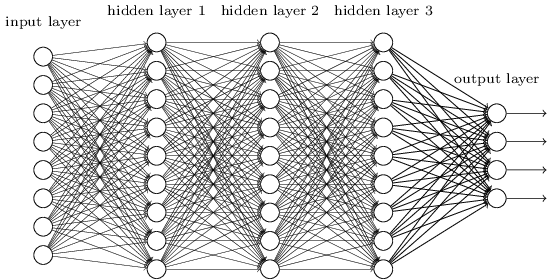
\includegraphics[scale=0.7]{neuralnetwork}
		\caption{Fully Connected Neural Network
			\label{nn-fully-connected}}
	\end{figure}
	\subsection{Loss Functions}
	Deep learning involves the process of minimizing or maximizing some function $f(x)$ by varying $x$\cite{Goodfellow-et-al-2016}, this is known as optimization and the function we want to optimize is known as the objective functions, cost function or loss function. Typically, our model consists of a distribution $P(y | x, \theta)$ and we use what is known as the \textit{principle of maximum likelihood} to arrive at the discrepancy also known as the \textit{cross-entropy} between the training data and the approximated function's predictions as a representation of the loss function. This is elaborated further below
	\subsubsection{Maximum Likelihood Estimation}
	This method was derived from wanting to have some principle from which we could generate specific loss functions that work for different models. Consider a a collection of training data that consists of $m$ separate examples, $\mathbb{X} = \{x_1, x_2, ..., x_m\}$. Since $\mathbb{X}$ is a representation of the true distribution $P_{data}$, we can assume that each $x_i$ is valid independently of each other. Let $P_{model}(x|\theta)$ be a parameterized probability distribution over the same space but now indexed by $\theta$, then $P_{model}(x|\theta)$ will map any input $x$ to a real number that estimated the true probability $P_{data}(x)$. The maximum likelihood parameter $\theta$ is then:
	\begin{align}
	&\theta_{ML} = \arg\max_{\theta}P_{model}\big(\mathbb{X}|\theta\big)\nonumber\\
	& = \arg\max_{\theta}\prod_{i=1}^{m}P_{model}\big(x_i|\theta\big)
	\end{align}		
	To simplify the above we take the logarithm of the likelihood as it does not alter the $\arg\max$ but only transform the product to a sum:
	\begin{align}
	& \theta_{ML}=\arg\max_{\theta}\sum_{i=1}^{m}\log P_{model}\big(x_i|\theta\big)
	\end{align}
	Since the $\arg\max$ is invariant to rescaling, we further divide by $m$ to obtain a general loss function that is represented by the \textit{expectation} with respect to the true distribution $P_{data}$ that is given by the training data:
	\begin{align}
	& \theta_{ML} = \arg\max_{\theta}\mathbb{E}_{x\sim P_{data}}\big[\log P_{model}\big(x|\theta\big)\big]
	\end{align}
	The above equation can now be interpreted as the process of minimizing the discrepancy between the true data $P_{data}$ defined by the training data and model distribution $P_{model}$ defined by the predictions of the model. The degree of this dissimilarity is called the \textit{Kullback Leibler} divergence or more commonly as KL divergence. This is given by :
	\begin{align}
	D_{KL}\big(P_{data}||P_{model} \big) = \mathbb{E}_{x\sim P_{data}}\big[\log P_{data}\big(x\big) - \log P_{model}\big(x\big)\big]
	\end{align}
	Since the term $\log P_{data}\big(x\big)$ is not a function of the model and is known, to minimize the KL divergence means that we need to only minimize:
	\begin{align}
	- \mathbb{E}_{x \sim P_{data}}\big[\log P_{model}\big(x\big)\big]
	\end{align}
	Thus minimizing the KL divergence is analogous to minimizing the cross-entropy between the distributions.
	\subsubsection{Approximating Conditional Distributions with Maximum Likelihood}
	As we saw is the previous section the Maximum Likelihood is the negative log-likelihood, also known as the cross-entropy between the training data and model predictions. Typically Neural Networks are training using this principle. This implies that a general loss function can be represented as :
	\begin{align}
	J\big(\theta\big) = -\mathbb{E}_{x,{y \sim P_{data}}}\log P_{model}\big(y|x\big)
	\end{align}
	The specific form can change between different models and depend largely on the structure of $\log P_{model}$. Further it can be shown that the loss function is invariant to terms that do not depend on the model parameters and thus can be discarded. That is if $P_{model}(x | y) = F(y, f(x,\theta), I)$ where $I$ represents the extra terms, then we arrive at the mean squared error cost:
	\begin{align}
	J\big(\theta\big) = \frac{1}{2} \mathbb{E}_{x,{y \sim P_{data}}} [\![y - f\big(x, \theta\big)]\!]^2 + \text{const} \label{eq:mse_loss}
	\end{align}
	Thus we can see that the equivalence between the maximum likelihood loss and the minimization of mean squared error holds for not only linear models but for any $f(x,\theta)$. A major advantage with this method is that we can avoid the the effort needed to generate cost functions for each different model, letting us automatically generate a loss function $\log P(x | y)$ for any model $P(x | y)$
	\subsection{Output Units}
	In the case of Neural Networks there seems to be a close relationship between the type of loss function chosen and the type of units used in the output layer of the network. Generally all types of neural network units can be used anywhere in the network and not only the output, here we focus on the use of these units as outputs. Consider a complex set of training data that includes some \textit{hidden} features described by $h = f(x,\theta)$. The function of the output is then to handle these features, generally by additional transformation from the features to the labels to arrive at good predictions.
	\subsubsection{Linear Units}\label{linear_unit}
	An affine transformation is one where points, straight lines and planes are preserved. One of the simplest types of units are called linear units and is based on affine transformations without any non-linearity. Given that we have features $h$, a layer of this type of unit generates a vector $\hat{y} = W^T h + b$. These output layers generally employed to generate the mean of a conditional distribution $P(y | x) = \aleph(y | \hat{y}, I)$, then maximizing the log-likelihood is analogous to minimizing the mean squared error.
	\subsubsection{Sigmoid Units}		
	It is common to find machine learning tasks that have a need to predict a binary variable $y$. The approach using maximum likelihood involves the definition of a Bernoulli Distribution over $y$ depending on $x$. This distribution is defined by a number and the neural network has to only predict whether $P(y=1 | x)$ and for this to be a valid probability it must lie in the interval $\big[0,1\big]$. Due to these constraints we use an approach that combines the sigmoid unit with the maximum likelihood. Thus a sigmoid output unit is defined by 
	\begin{equation}
	\hat{y} = \sigma\big(w^T h + b\big)
	\end{equation}
	where $\sigma$ is the logistic sigmoid, defined by $\sigma(x) = \frac{1}{1 + e^{-x} }$. We can interpret this as the output unit having two distinct components. First a linear layer is used to compute $\big(w^T h + b\big)$. Then, the logistic sigmoid is used to convert this into a probability.
	\subsubsection{Softmax Units}		\label{softmax}
	The softmax output is used in situations where a probability distribution over a discrete variable with $n$ different possible values needs to be modeled. For example in the case of representing a mapping between actions and states of a RL Agent where there are $n$ different states. Thus softmax functions are generally employed as outputs of classifiers to represent the distribution over $n$ different classes. These type of outputs can also be considered as a generalization of the above sigmoid function. With the sigmoid we only had to 2 classes of outputs $0$ and $1$, to generalize this to the case of $n$ different values we require a vector $\hat{y}$ such that $\hat{y_i} = P\big(y=i | x\big)$. Here not only each element of $\hat{y_i}$ is to be between 0 and 1, but the entire vector $\hat{y}$ should also sum to 1 to make it represent a valid probability. To do this we first consider a linear layer that predicts raw log probabilities:
	\begin{align}
	z = W^T h + b 
	\end{align} 
	where $z_i =\log \tilde{P}(y = i | x)$, here $\tilde{P}$ represents an unnormalized probability distribution. We then exponentiate and normalize $z$ to get the desired $\hat{y}$. Thus :
	\begin{align}
	\text{softmax}\big(z\big)_i = \frac{\exp\big(z_i\big)}{\sum_{j}\exp\big(z_i\big)}
	\end{align}
	Now we need to maximize $\log P(y=i;z) = \log \text{softmax}(z)_i $ Applying log-likelihood we get:
	\begin{align}
	\log \text{softmax}\big(z\big)_i = z_i - \log \sum_{j}\exp\big(z_j\big)
	\end{align}
	Thus the softmax units helps us to handle cases where there $n$ separate output classes.
	\subsection{Hidden Units}
	Previously we saw the various design choices for MLPs that are actually common to most ML models that use gradient based training methods. Now we consider the types of units used in hidden layers which is unique to MLPs. Typically hidden units can be represented as some vector of inputs $x$ that has a linear affine transformation applied on it $z = W^Tx + b$. To this transformation some element-wise non-linear function $g(z)$ is applied. Typically hidden units only vary the activation function $g(z)$.
	\subsubsection{Rectified Linear Units(ReLU)}
	Earlier we discussed the Linear Unit in Section \ref{linear_unit}. The difference between a rectified linear unit and a linear unit is that for half of its domain the ReLU will give an output of zero. Thus the output activation function that ReLU's use is of the form $g(z) = \max \{0,z\}$. From this function we can intuitively see that the derivatives through a ReLU remains large while the unit is active. Further the second derivative of this operation outputs zero everywhere. As discussed the ReLUs are generally used after an affine linear transformation. Thus we have
	\begin{equation}
	h = g\big(W^Tx + b\big)
	\end{equation}
	When using ReLUs we generally set the parameters of the transformation such that all elements of $b$ and the weights hold a small positive value. This ensures that the ReLU is active for most inputs in the training data and allows the derivatives to pass. The plot of the rectifier $g(z)$ can be seen in Figure \ref{relu}
	\begin{figure}[H]
		\centering
		\setlength{\fboxsep}{5pt}%
		\setlength{\fboxrule}{1pt}%
		\fbox{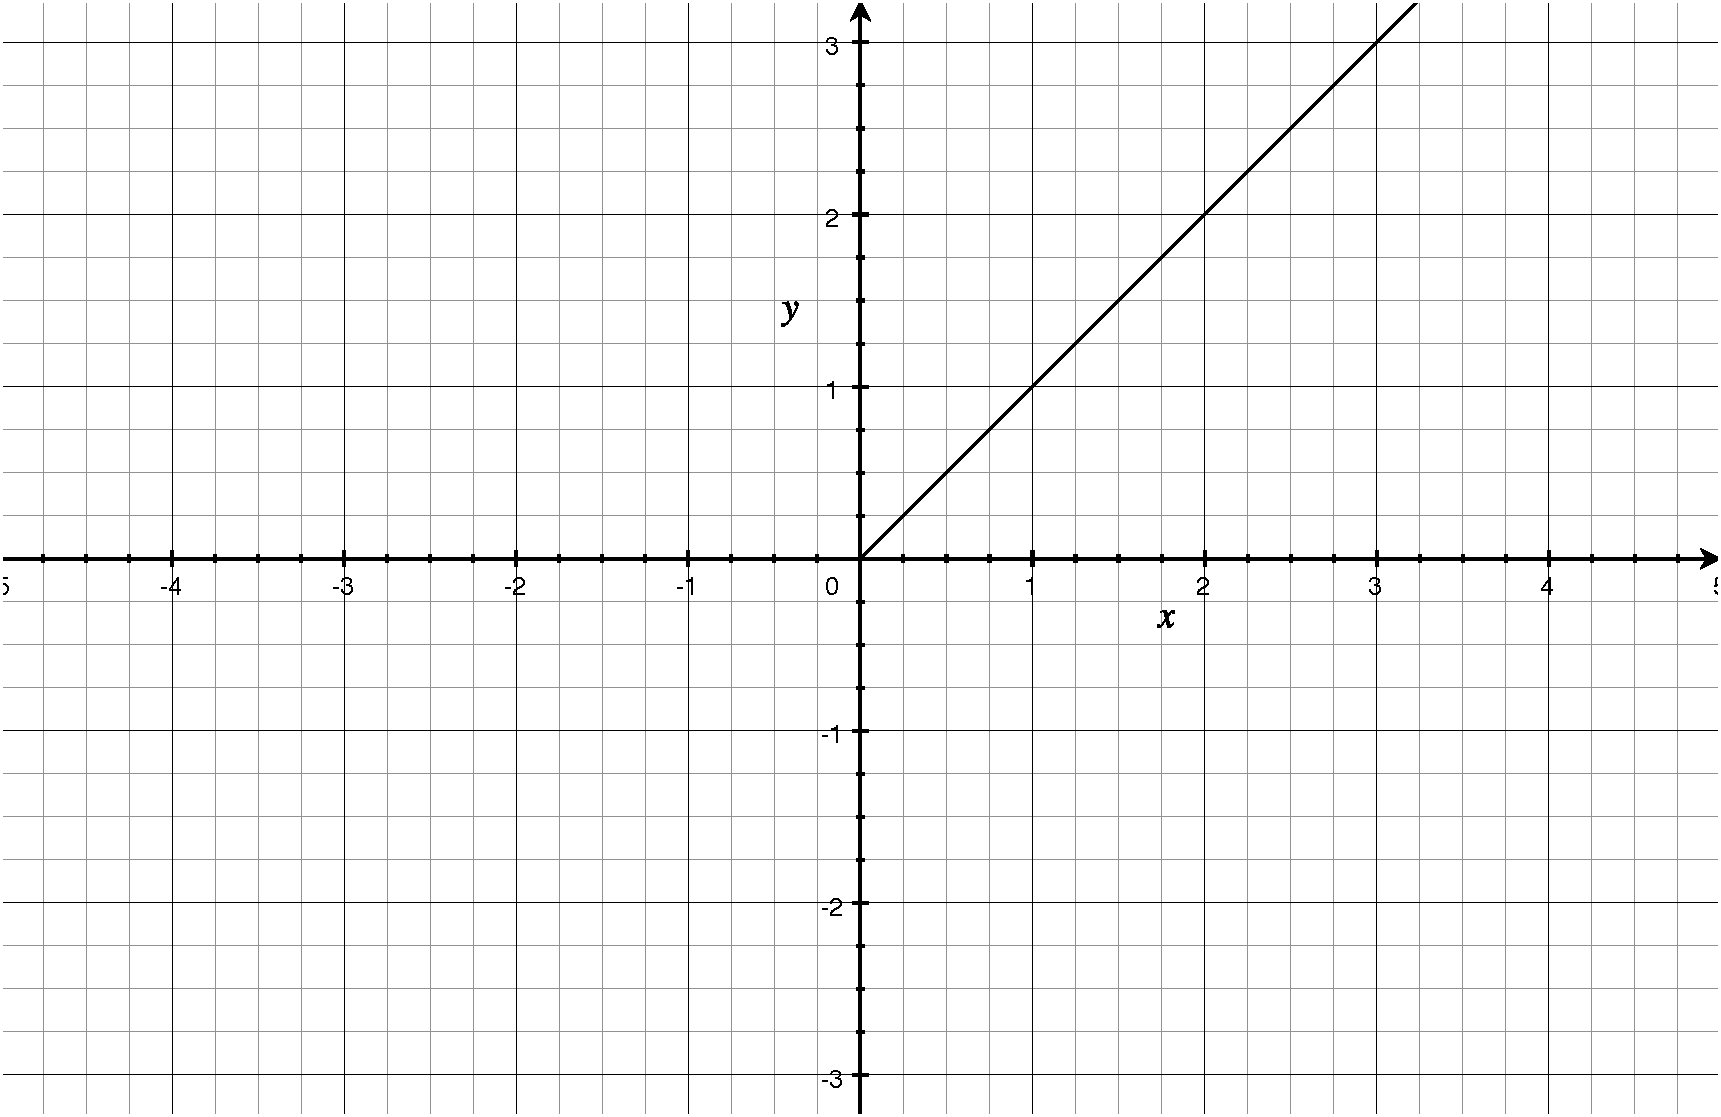
\includegraphics[scale=0.4]{relu}}
		\caption{Rectified Linear Unit
			\label{relu}}
	\end{figure}
	One major drawback of ReLUs is that if the examples in the training set cause its activation to be pushed to zero then no learning is performed, some generalizations of ReLUs were later designed to ensure a gradient everywhere. These generalizations of ReLUs, whose performance is generally comparable to that of the vanilla ReLU are typically based on a non-zero slope $\alpha_i$ when $z_i < 0$. This gives us  $h_i = g(z_i,\alpha)_i = \max(0,z_i) + \alpha_i \min(0,z_i)$. A popular generalization of ReLUs that is found to be very effective with image recognition tasks is called the \textit{Absolute Value Rectifier} \cite{jarrett2009best}. This Absolute Value Rectifier pushes $g(z) = |z| $ by fixing $\alpha_i = -1$. Other typical generalizations of ReLUs are widely used across various task domains. These include the \textit{Leaky} ReLU that sets $\alpha_i$ to a small positive value like $0.01$\cite{maas2013rectifier}. Further the Parametric ReLU lets $\alpha_i$ be learnt during training\cite{he2015delving}.
	\subsubsection{The Hyperbolic Tangent and Logistic Sigmoid}
	The ReLU we learnt about in the previous section is actually in use only recently. Prior to their invention, most neural networks and other ML algorithms that use gradients for optimization used the logistic sigmoid or the hyperbolic tangent activation functions described below.
	The sigmoid activation function is of the form,
	\begin{equation}
	g\big(z\big) = \sigma\big(z\big)
	\end{equation}
	And hyperbolic tangent activation function is represented by,
	\begin{equation}
	g\big(z\big) = \tanh\big(z\big)
	\end{equation}
	Further the above functions are closely related due to the relation $$\tanh\big(z\big) = 2\sigma\big(2z\big) - 1$$
	Previously we discussed sigmoid units used as outputs to predict binary classification results. Sigmoidal units, unlike element-wise linear units saturate to a high value when $z$ is very positive and go to a low value when $z$ is negative, the plot of the sigmoid function can be seen in Figure \ref{sigmoid}. When $z$ is near 0, the sigmoidal becomes strongly sensitive to the input. Due to this saturation, they often make gradient based learning difficult and thus their use as hidden units is generally discouraged in the field.
	\begin{figure}[H]
		\centering
		\setlength{\fboxsep}{5pt}%
		\setlength{\fboxrule}{1pt}%
		\fbox{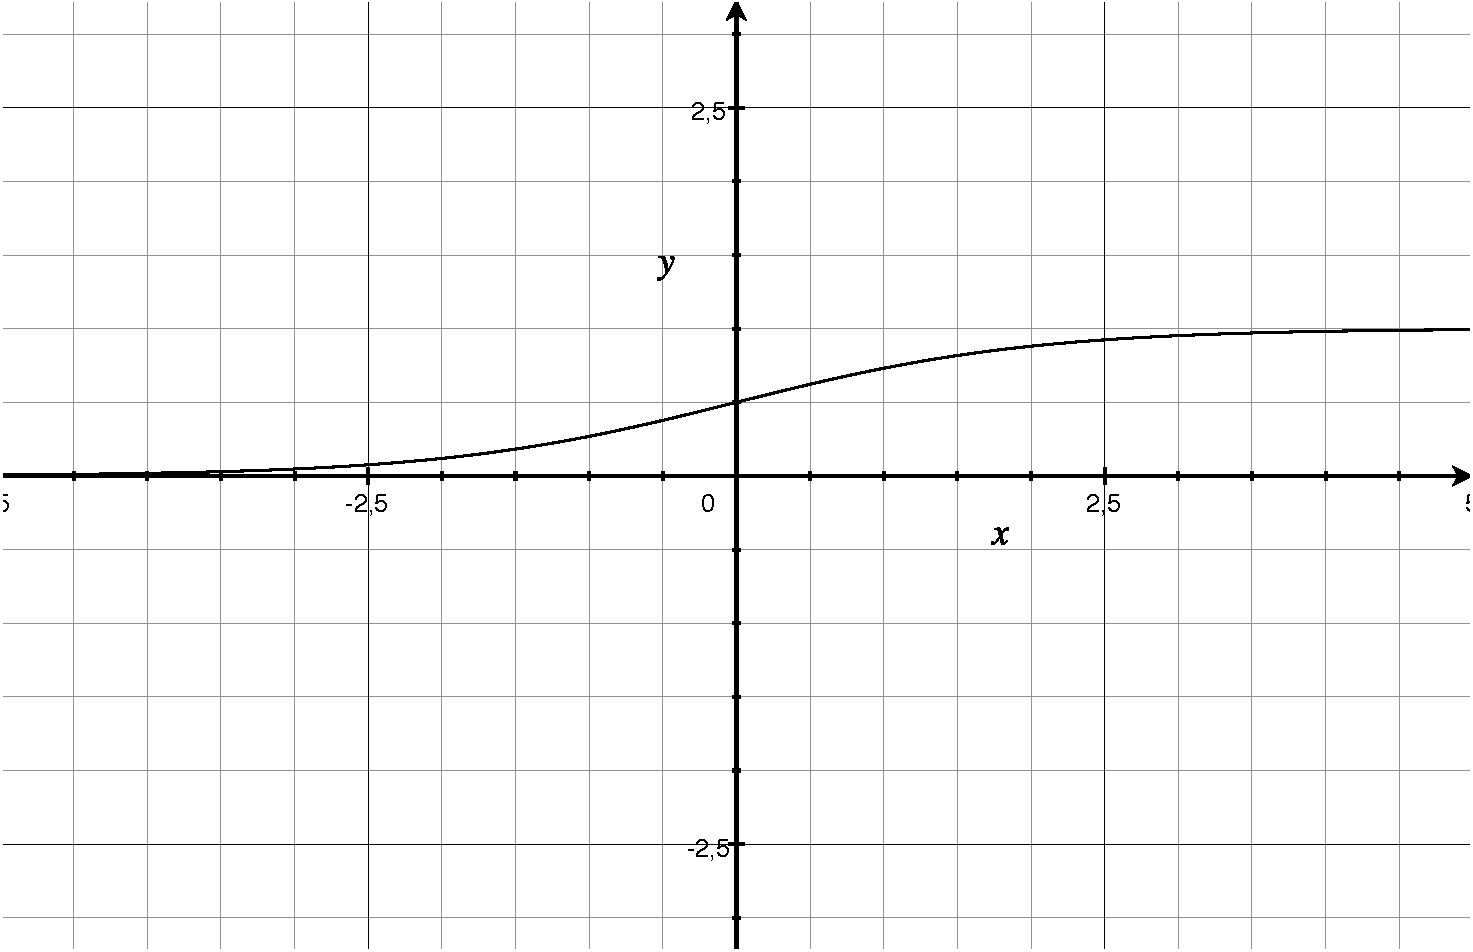
\includegraphics[scale=0.4]{sigmoid}}
		\caption{Logistic Sigmoid Unit
			\label{sigmoid}}
	\end{figure}
	Typically the hyperbolic tangent activation performs better than the sigmoid. Due to the fact that $\tanh(0) = 0$ while $\sigma(0) = 0.5$, the hyperbolic tangent resembles the identity function closely as we approach 0, this can be seen in Figure \ref{tanh}. Training a network $\hat{y} = w^T\tanh(U^T\tanh(V^Tx))$ is similar to training a simple linear model $\hat{y} = w^TU^TV^Tx$ given that the activations of the network can be kept small and manageable, this makes training with tanh more efficient.
	\begin{figure}[H]
		\centering
		\setlength{\fboxsep}{5pt}%
		\setlength{\fboxrule}{1pt}%
		\fbox{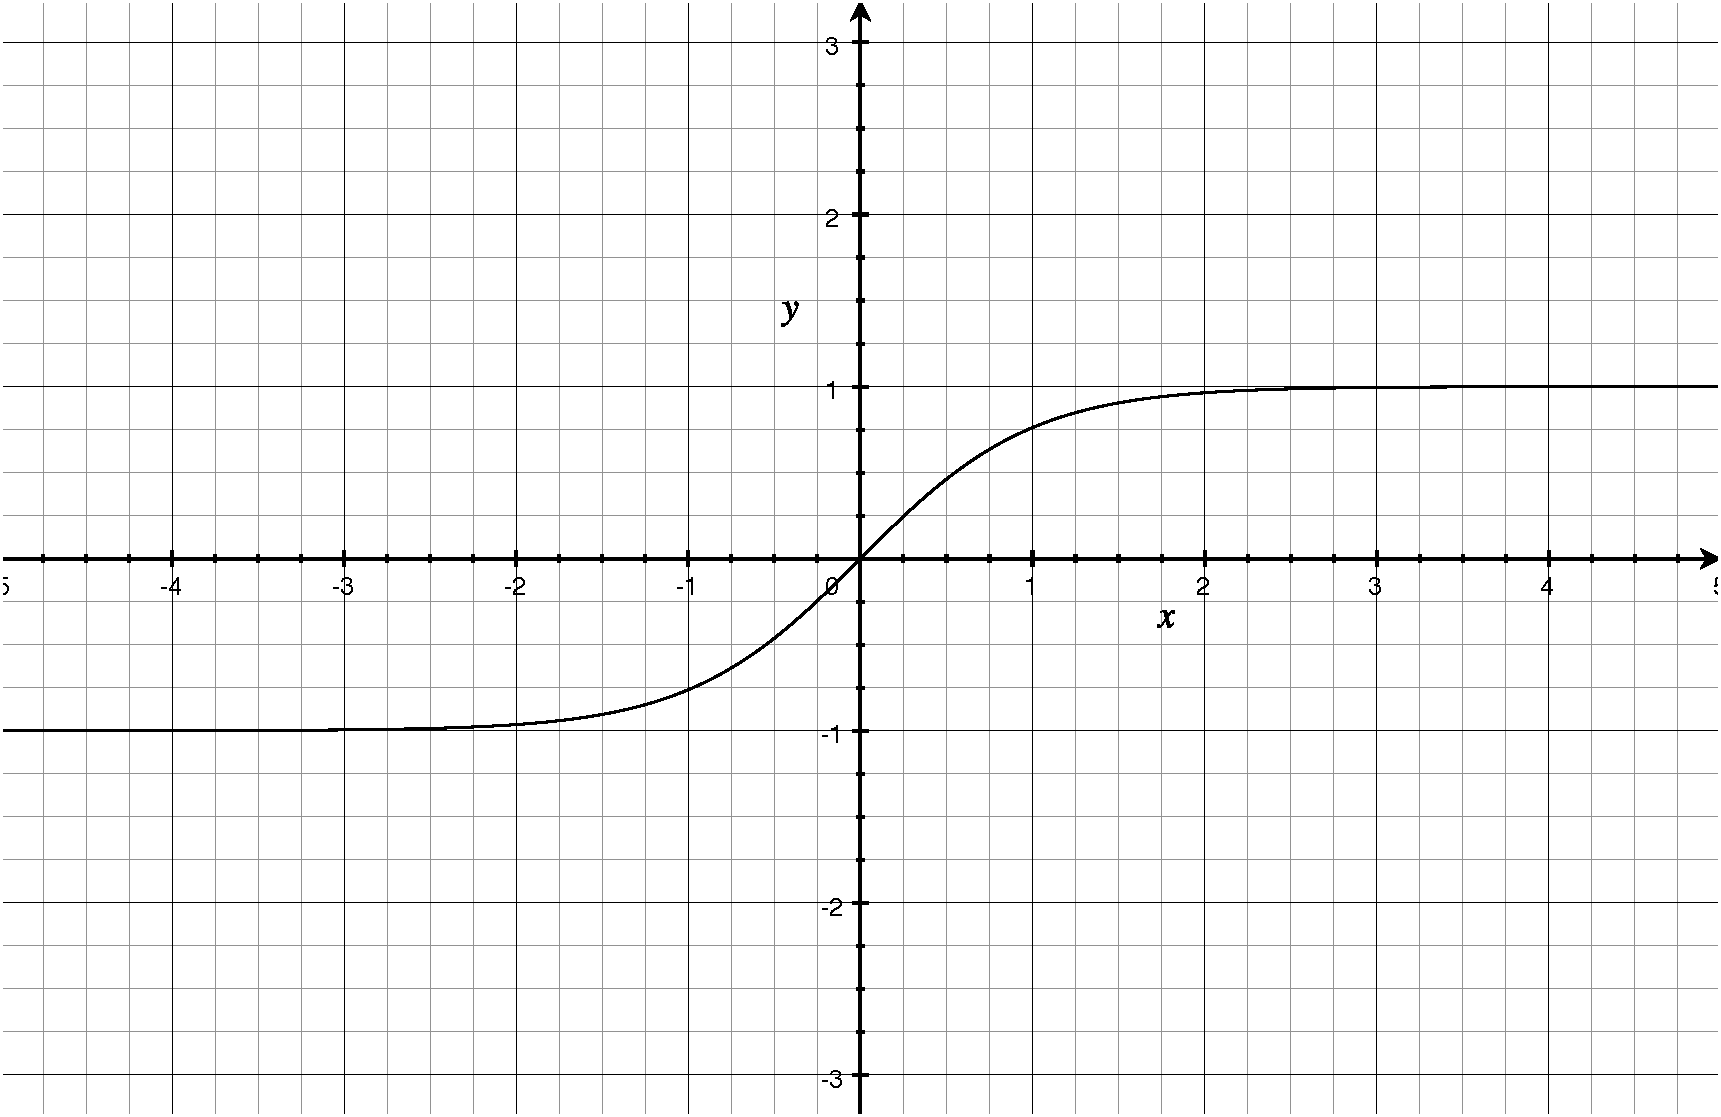
\includegraphics[scale=0.35]{tanh}}
		\caption{Hyperbolic Tangent Unit
			\label{tanh}}
	\end{figure}
	\subsection{Architecture}
	Previously we saw the internal workings of the MLP, the design and working of its internal components and cost functions. Now we focus on two main questions, the solution of which forms the architecture of a MLP. These are typically how many units should it have(the \textit{width} of the network) in how many successive layers(the \textit{depth} of the network). Here layers are groups of units or neurons which are typically arranged into a chain like structure with each successive layer being fed the output of the previous layer or, each layer is a function of the preceding layer. In these chain like structures the index gives the position of the layer it belongs to, Such that $$h^{(1)} = g^{(1)}(W^{(1)T}x + b^{(1)})$$ represents the first layer and $$h^{(2)} = g^{(2)}(W^{(2)T}x + b^{(2)})$$ represents the second\cite{Goodfellow-et-al-2016} and so on. This is illustrated in Figure \ref{nn_arch} where we can see a neural network with a depth of 3 consisting of a single output layer with 4 units, a single hidden layer with 3 units and an output layer with 1 unit.
	\begin{figure}[H]
		\centering
		\setlength{\fboxsep}{5pt}%
		\setlength{\fboxrule}{1pt}%
		\fbox{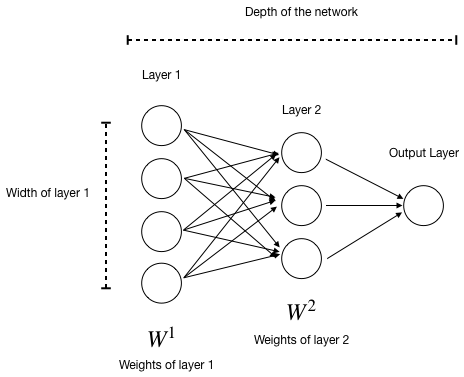
\includegraphics[scale=0.6]{nn-arch}}
		\caption{General Architecture of a Neural Network
			\label{nn_arch}}
	\end{figure}
	\subsection{Gradient Based Learning}		
	Typically Machine Learning algorithms involves the task of optimizing, which means the process of maximizing and minimizing a function (generally a loss function) $f(x)$ by repeatedly altering $x$\cite{Goodfellow-et-al-2016}.
	Consider some function $y = f(x)$, with $x, y \in \mathbb{R}$. We know that the derivative of this function is given by $f'(x) $ or $\frac{dy}{dx}$ and represents the slope of $f(x)$ at a certain point $x$. In essence, this tells us how by making a small change in $x$ we can get a corresponding change in $y$ or how the output can be pushed in a certain direction according to changes in the input: $f(x + \epsilon) \simeq f(x) + \epsilon f'(x)$.  Thus the derivative is important in the process of optimization as it tells us how to improve $y$ by changing $x$ allowing us to reduce $f(x)$ by moving $x$ in small steps with the opposite sign of the computed derivative. Invented by the mathematician Cauchy in 1847 \cite{cauchy1847methode}, this process, illustrated in Figure \ref{grad_descent}\footnote{http://www.deeplearningbook.org/contents/numerical.html, Page 81}, is fundamental to many Machine Learning Algorithms and central to Deep Learning where it is known as \textit{Gradient Descent}.
	\begin{figure}[h]
		\vspace{0.2cm}
		\centering
		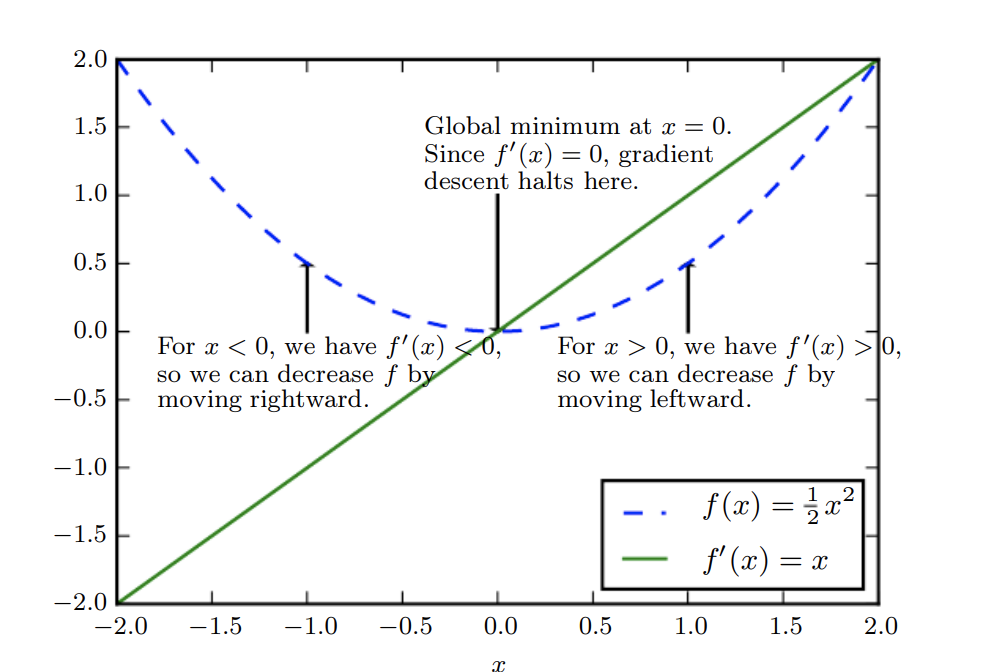
\includegraphics[scale=0.8]{grad_descent}
		\caption{The Process of Gradient Descent\cite{Goodfellow-et-al-2016}
			\label{grad_descent}}
	\end{figure}
	\pagebreak
	\subsubsection{Back-Propagation}	
	As we now know a feedforward neural network produces an output $\hat{y}$ for an input $x$, this process involves a flow of information through the layers of the network. The information provided by $x$ is \textit{propagated} to the units at each layer and consequently generates $\hat{y}$. This process is known as \textit{forward propagation}. This propagation continues until finally a scalar loss $J(\theta)$ is produced (by comparing y and $ \hat{y}$). Now in order to apply gradient descent or any other gradient based learning algorithm, we need to compute the gradient of this loss. This is achieved by letting the information flow from the loss, backward through the network. This process is known as \textit{back-propagation}\cite{rumelhart1986learning} and is illustrated in Figure \ref{back_prop}. Thus the back-propagation algorithm is only the technique used to compute the gradient, and some other algorithm such as Stochastic Gradient Descent uses this gradient to perform learning. 
	\begin{figure}[H]
		\centering
		\setlength{\fboxsep}{5pt}%
		\setlength{\fboxrule}{1pt}%
		\fbox{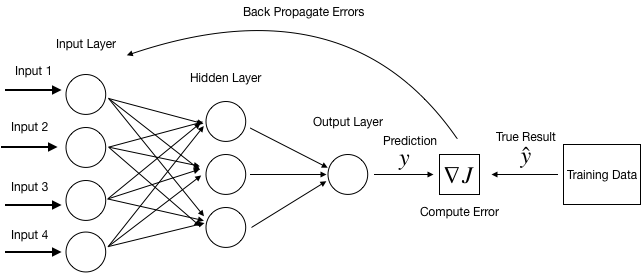
\includegraphics[scale=0.7]{back_prop}}
		\caption{Back Propagating Errors Through a Neural Network
			\label{back_prop}}
	\end{figure}
	Here we formally express the process of computing the gradient $\nabla_{x}f(x,y)$ for some function $f$, with $x$ as a set of variables whose derivatives we need and $y$ as a set of inputs to the function. In the case of learning algorithms, we use the gradient of the loss function we discussed above based on the weights of the network$\nabla_{\theta}J(\theta)$.
	Now we consider forward and back propagation for the layers of a fully connected MLP. In Algorithm \ref{alg:forward-prop} we see the process of forward-propagation. This process performs a mapping between a single training example ($\text{Input}=x, \text{Target}=y$). Here the loss $L(\hat{y},y)$ depends directly on the output of the final layer $\hat{y}$ and the label of the current input $y$. Typically a regularizer $\Omega(\theta)$ is added before computing the total loss $J$, where the parameter $\theta$ describes the weights and biases of the network.
	\begin{algorithm}[H]
		\DontPrintSemicolon
		\SetAlgoLined
		\SetKwInOut{Parameter}{Require}
		\SetKwInOut{Input}{Input}\SetKwInOut{Output}{Output}
		\Parameter{Network depth, $l$}
		\Parameter{$W^{\big(i\big)}, i \in \{1,...,l\}$, the weight vectors of the network}
		\Parameter{$b^{\big(i\big)}, i \in \{1,...,l\}$, the bias parameters of the network}
		\Parameter{$x$, the input to process}
		\Parameter{$y$, the target output}
		\BlankLine
		$h^{(0)} = x$\;
		\For{$k = 1,...,l$}{
			$a^{(k)} = b^{(k)} + W^{(k)}h^{(k-1)}$\;
			$h^{(k)} = f(a^{(k)})$\;
		}
		$\hat{y} = h^{(l)}$\;
		$J = L(\hat{y},y) + \lambda	\Omega(\theta)$
		
		\caption{Forward Propagation through a deep neural network and the loss computation}\label{alg:forward-prop}
	\end{algorithm}
	
	Above we saw the process used to propagate information in the forward direction though a deep neural network and the consequent computation of the loss. Now to perform gradient-based learning we need to compute the gradient of this loss $\nabla J$ with respect to the neural network parameters $W$ and $b$, this back-propagation process can be seen in Algorithm \ref{alg:back-prop}. here our aim is to generate the gradients on the activations $a^(k)$ for every layer $k$, but this time going backwards, starting from the output layer and going toward the input layer. From the computed gradients, we can get a picture of how the parameters of each layer should be varied in order to move the predicted result $y$ closer to the true target $\hat{y}$.
	\begin{algorithm}[H]
		\DontPrintSemicolon
		\SetAlgoLined
		\SetKwInOut{Parameter}{Require}
		\SetKwInOut{Input}{Input}\SetKwInOut{Output}{Output}
		After the forward propagation, compute the gradient on the output layer\;
		$g \leftarrow \nabla_{\hat{y}}J = \nabla_{\hat{y}}L(\hat{y}, y)$\;
		\For{$k = l,l-1,...,1$}{
			Convert the grdient on the layer's output into a gradeint on the activation function\;
			$g \leftarrow \nabla_{a^k}J = g \odot f'(a^k)$\;
			Compute gradients on weights and biases:\; 
			$\nabla_{b^{(k)}}J = g + \lambda \nabla_{b^{(k)}}\Omega(\theta)$\;
			$\nabla_{W^{(k)}}J = g h^{(k-1)T} + \lambda\nabla_{W^{(k)}} \Omega(\theta)$\;
			Propagate the gradients w.r.t the next lower-level hidden layer's activations:\;
			$g \gets \nabla_{h^{(k-1)}}J = W^{(k)T}g $\;
		}
		\caption{Back Propagation}\label{alg:back-prop}
	\end{algorithm}
	\subsubsection{Stochastic Gradient Descent(SGD)}\label{sgd}
	One of the most widely used optimization algorithms in this field is SGD. Earlier we saw the process of Gradient Descent where we used a derivative of a function to descend downhill by making small changes in the input. This process is strengthened by using SGD to follow the gradient of small batches of data downhill to reduce the loss. For this algorithm we use small batches of data known as mini-batches, which let us compute the estimate of the gradient by averaging over a mini-batch of $m$ examples. An important hyper-parameter for SGD is the \textit{learning rate}. Practically when training a neural network it is required to gradually decrease the learning rate as time passes, this here we represent the learning rate as $\epsilon_k$ for the $k$-th iteration. The reason behind this learning rate \textit{decay} is the noise generated from randomly sampling $m$ examples at a time (using mini-batches) stays active even when we successfully minimize the loss. The below Algorithm shows the process of SGD: 
	\begin{algorithm}[H]
		\DontPrintSemicolon
		\SetAlgoLined
		\SetKwInOut{Parameter}{Require}
		\SetKwInOut{Input}{Input}\SetKwInOut{Output}{Output}
		\Parameter{Learning Rate Schedule, $\epsilon_1, \epsilon_2, \dots$}
		\Parameter{Initial Parameter $\theta$}
		$k \gets 1$\;
		\While{Not Stopping Criteria}{
			Sample $m$ examples from training set $\{x^{(1)},\dots ,x^{(m)} \}$ with respective targets $y^{(i)}$\;
			Compute Gradient: $\hat{g} \gets \frac{1}{m}\nabla_{\theta}\sum_{i}L(f(x^{(i)};\theta), y^{(i)})$\;
			Apply Update: $\theta \gets \theta - \epsilon_k \hat{g}$\;
			Increment $k$: $k \gets k + 1$ 
		}
		\caption{Stochastic Gradient Descent Algorithm}\label{alg:sgd}
	\end{algorithm}
	
	\begin{align}
	&\text{Further, a sufficient condition to ensure the convergence os SGD is : }\nonumber\\
	&\sum_{k=1}^{\infty}\epsilon_k = \infty \text{,     {}{}    and}\\
	&\sum_{k=1}^{\infty}\epsilon_k^2 < \infty
	\end{align}
	\pagebreak
	
	\section[Neural Dialog Management]{Neural Dialog Management  with Deep Reinforcement Learning}\label{dm-with-drl}
	\subsection{Overview}
	Previously we saw how we can develop dialog strategies by applying Policy and Value Iteration Methods. In this chapter we will see the implementation of Algorithms from these methods, specifically the Advantage Actor Critic Algorithm applied to learn simple dialog strategies.	What we mean by Neural Dialog Management. What are actor critic methods (refer section 4.5.3). How is it conceptually applied to dm, like what does the critic do actor do with respect to dialog and what does the critic do with respect to dialog.
	\subsection{REINFORCE}
	In Section \ref{policy_methods} we learnt about finding the gradient of the objective loss of a parameterized policy i.e.\ the policy gradient. We now use the policy gradient we derived in Equation \ref{eq:vpg_update} to build a PG learning algorithm. This is known as the REINFORCE algorithm or Monte Carlo Policy Gradient algorithm\cite{Williams92REINFORCE}. For the parameterization we use a deep neural network to approximate the policy $\pi_{\theta}$ where $\theta$ represent the weights of the network. The PG theorem gives us an expression (Equation \ref{eq:vpg_update}) that is exactly equal to the gradient of the loss or performance measure of the parameterized policy. To use this method for actual learning we need a way to sample the episodes of the environment such as the expectation of the samples for each episodes is approximately equal to this expression i.e\ RHS of Equation \ref{eq:vpg_update}. With a little further investigation we can also see that the RHS of the PG theorem is a sum over the states weighted by the recurrence rate of these states i.e\ how often we see these states under the required policy $\pi$. Thus we have 
	\begin{align}
	&\nabla_{\theta}J\big(\theta\big)\propto \sum_{s}d_{\pi}\big(s\big)\sum_{a}q_{\pi}\big(s,a\big)\nabla_{\theta} \pi_{\theta}\big(a|s\big)\nonumber\\
	& = \mathbb{E}_{\pi}\big[\sum_{a}q_{\pi}\big(s_t,a\big)\nabla_{\theta}\pi_{\theta}\big(a|s_t\big)\big]\label{eq:pg-expectation}
	\end{align}
	Now in the remaining part of the expectation above is a sum over actions i.e.\ $\sum_{a}\nabla_{\theta}\pi_{\theta}\big(a|s\big)$. To make it such that the action in the above equation $a$ represents the sample of actions $a_t$ we must make sure that each term above is weighted by the probability of selecting those actions i.e.\ by $\pi_{\theta}\big(a_t|s_t\big)$.
	\begin{align}
	&\nabla_{\theta}J\big(\theta\big) = \mathbb{E}_{\pi}\bigg[\sum_{a}\pi_{\theta}\big(a|s_t\big)q_{\pi}\big(s_t,a\big)\frac{\nabla_{\theta}\pi_{\theta}\big(a|s_t\big)}{\pi_{\theta}\big(a|s_t\big)} \bigg]
	\end{align}
	Now we can replace $a$ by sample action $a_t$
	\begin{align}
	&\nabla_{\theta}J\big(\theta\big) = \mathbb{E}_{\pi}\bigg[q_{\pi}\big(s_t,a_t\big)\frac{\nabla_{\theta}\pi_{\theta}\big(a_t|s_t\big)}{\pi_{\theta}\big(a_t|s_t\big)} \bigg] \nonumber \\
	&=\mathbb{E}_{\pi}\bigg[G_t\frac{\nabla_{\theta}\pi_{\theta}\big(a_t|s_t\big)}{\pi_{\theta}\big(a_t|s_t\big)} \bigg],\ \text{Since} \  \mathbb{E}_{\pi}\big[G_t|s_t,a_t\big] = q_{\pi}\big(s_t,a_t\big)
	\end{align}
	Here $G_t$ is the total return for one episode. This final expression is a quantity that can be sampled on for the steps of each episode and whose expectation is equal to the policy gradient. Thus we can define an update rule for the parameterized weights as:
	\begin{align}
	&\theta_{t+1} = \theta_t + \alpha G_t\frac{\nabla_{\theta}\pi_{\theta}\big(a_t|s_t\big)}{\pi_{\theta}\big(a_t|s_t\big)} \label{eq:reinforce-update}
	\end{align}
	This is called the REINFORCE algorithm and the above expression is its update with $\alpha$ being its learning rate. Intuitively here we can see that each increment to the weights is directly proportional to the product of the return and the gradient of the probability of taking the action that was taken divided by the probability of taking that very action. Thus this update pushes this second term which is a vector in the direction proportional to the return and inversely proportional to the probability of taking that action. We do this as we can then move the parameter in the direction which produce the action that yield the highest possible return and because we can give lesser importance to the most frequently selected actions as they may not lead to the highest returns. Since this algorithm uses the total return from that starting time step of an episode $t$ which includes all rewards until the end of the episode i.e.\ performs a full backup, this is also known as Monte Carlo Policy Gradient
	\subsubsection{REINFORCE Algorithm}\label{reinforce}
	Using the update rule we derived in the previous section i.e.\ Equation \ref{eq:reinforce-update} we can build the full REINFORCE algorithm and process as shown in Algorithm \ref{alg:reinforce}
	\begin{algorithm}
		\DontPrintSemicolon
		\SetAlgoLined
		\SetKwInOut{Parameter}{Require}
		\SetKwInOut{Sample}{Sample}
		\SetKwInOut{Input}{Input}\SetKwInOut{Output}{Output}
		\Input{Differentiable Policy Parameterization $\pi(a|s, \theta)$}
		\Parameter{Initialize Policy Parameter $\theta$}
		\While{$S$ is not Terminal}{
			Generate an episode on policy $\pi_{\theta}$: $s_0,a_0,r_1,...,s_{t-1},a_{t-1},r_t$\;
			\For{Each Step of the episode $t=0,...,T$}{
				$G_t \gets $ Return at time $t$\;
				Update Policy Parameters : $\theta \gets \theta + \alpha\gamma^t G_t \nabla_{\theta}\ln\pi_{\theta}(a_t|s_t)$	
			}
			
		}
		\caption{REINFORCE}\label{alg:reinforce}
	\end{algorithm}
	\subsubsection{Policy Network}
	
	The Policy Network approximates the policy $\pi_{\theta}(a| s)$ with parameter $\theta$ can be found in the above figure. It is a Neural Network with the following characteristics:
	\begin{itemize}
		\item Input Layer : The Input layer consists units with equal number to that of the dimensions of the state space. The Input is the observable state $S$. The Input Layer has a Rectified Linear Unit as its activation. Further the Input Layer is initialized with zero values for all its weights and biases. 
		\item Hidden Layers : The two Hidden layers consist of 32 and 16 neurons respectively. The hidden layers are fed from the output of th ReLU from the Input layers. Further each hidden layer has another ReLU as its activation. Both Hidden Layers are initialized with zero values for their weights and biases.
		\item Ouput Layer: The Output Layer consists of units with the same number as the dimension of the action space. The role of the output layer is to produce a probability distribution across the various possible actions so that we can choose the action with the highest probability. Thus we use a Softmax as the activation function from Section \ref{softmax} which can generate the required probability distribution across the $n$ actions in the action space. The Output Layer is also initialized with zero values for all its weights and biases.
		\item Loss Function: here we use the Mean Squared Error loss function, from Equation \eqref{eq:mse_loss}.
		\item Optimizer: For the learning algorithm we have used the Adaptive Moments Optimizer (Adam)\cite{kingma2014adam} which is a special form of the SGD Algorithm where the learning rate adapts to the magnitude of the partial derivative of the cost function. 
	\end{itemize}
	\begin{figure}[h]
		\vspace{0.2cm}
		\centering
		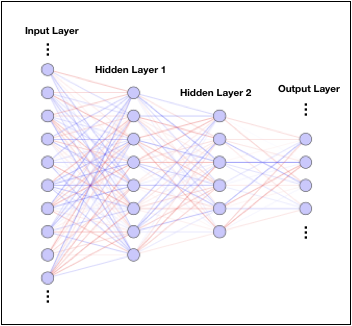
\includegraphics[scale=0.6]{nn-actor}
		\caption{Policy Neural Network
			\label{nn-policy}}
	\end{figure}
	\subsection{Advantage Actor Critic}	\label{a2c-section}
	The Advantage Actor Critic Algorithm is a hybrid method that combines both policy and value learning. This method involves the use of two neural networks. The first is called an \textit{Actor}: $\pi(a|s,\theta)$, this control how the RL agent behaves, in other works maps semantic states to actions. The other network is called a \textit{Critic}: $\hat{q}(s,a,w)$, which measures the value or quality of the action taken in the present state. Here $\theta$ and $w$ represents the parameters of their respective networks. This technique overcomes the drawback of the previous \textit{Vanilla} Policy Gradients such as a high degree of variance and the slow learning and time to convergence. This is done by introducing a better scoring function \cite{Sutton_pg}. A good candidate for this function is the learned value function or Critic as we have seen in Section \ref{section:ac-methods}. Typically the Critic is implemented using the Temporal Difference update algorithm and the Actor using the vanilla Policy Gradient update with the value function in its expectation from Equation \ref{eq:vpg_update} $q_{\pi}(s,a)$ by the Critic Network $\hat{q}_{\pi}(s,a,w)$ where $w$ represents the weights of the network and $\hat{q}$ represents the approximated value function. This method has a major drawback which is that value function approximation have a high degree of variance which is addressed by the \textit{Advantage function}. An overview of the entire Advantage Actor Critic process can be seen in Figure \ref{a2c}.
	\subsubsection{Advantage Function}
	To address the drawbacks of using value approximation directly in learning, the Advantage function was introduced \cite{Sutton_pg}. From Policy methods in Section \ref{policy_methods} we know that the objective is to find a parameterized policy $\pi_{\theta}(a|s)$ that can maximize the objective function, in this case the total expected discounted cumulative reward $J(\theta)$ starting from a certain dialog state over all possible dialog paths. Further, from the \textit{Policy Gradient Theorem}\cite{Sutton-introRL} we have the gradient of the objective function as:
	\begin{align}
	& \nabla_{\theta}J\big(\theta\big) = \mathbb{E}_{\pi}\big[q_{\pi}\big(s,a\big)\nabla_{\theta}\ln\pi_{\theta}\big(a|s\big)\big]\nonumber &&\big(\text{From Eq. \ref{eq:vpg_update}}\big) .
	\end{align}
	This representation of the gradient implies a potentially high degree of variance. This can be handled with the introduction of a comparison of the action-value to a baseline while not affecting the estimated gradient \cite{Sutton-introRL}. The value function is generally a good choice for this and thus Equation \ref{eq:vpg_update} becomes: 
	\begin{align}
	& \nabla_{\theta}J\big(\theta\big) = \mathbb{E}_{\pi}\big[\nabla_{\theta}\ln\pi_{\theta}\big(a|s\big)\big(q_{\pi}\big(s,a\big) - v_{\pi}\big(s\big) \big)\big].\label{eq:baseline}
	\end{align}
	Here the expression $\big(\hat{q}_{\pi}\big(s,a\big) - \hat{v}_{\pi}\big(s\big) \big)$ is known as the \textit{Advantage function} $A(s,a)$ and tells us the improvement in the action taken in a particular state compared to the average for that state. Thus if $A(s,a) > 0$ then our gradient of the objective function $\nabla_{\theta}J(\theta)$ is returning a value higher than the expected average for that state and thus is sent further in the same direction. If $A(s,a) < 0$, this means that our action returned a reward that was worse than the average for that state and thus the gradient is sent backward in the opposite direction. To implement this algorithm we need two value functions $\hat{q}_{\pi}(s,a)$ and $\hat{v}_{\pi}(s)$, this can be simplified by using the expression from Equation \ref{eq:9}.
	\begin{align}
	\hat{A}_{\pi}(s_t,a,w)  = R_{t+1} + \gamma \hat{v}_{\pi}\big(s_{t+1},w\big) - \hat{v}_{\pi}\big(s_t,w\big) \label{eq:adv}
	\end{align}
	where $s$ is the observed state of the dialog, $a$ is the chosen action, $t$ is the current time-step and $w$ is the parameters of the neural network (or any other function approximators) 
	\begin{figure}[h]
		\centering
		\setlength{\fboxsep}{5pt}%
		\setlength{\fboxrule}{1pt}%
		\fbox{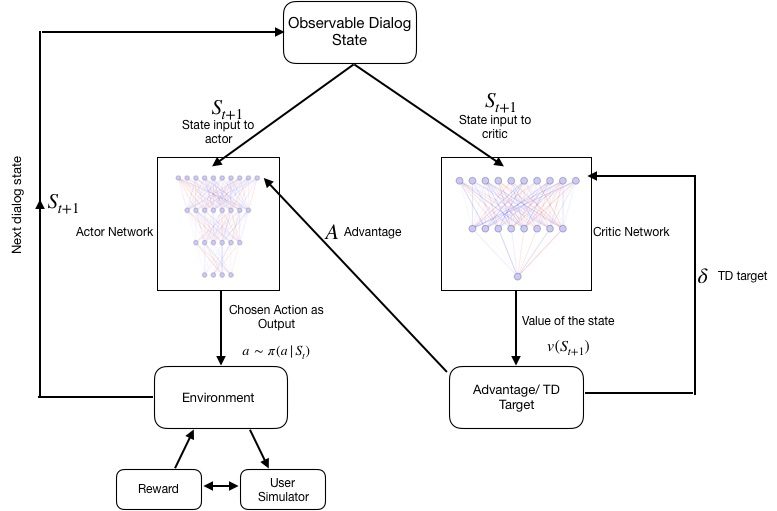
\includegraphics[scale=0.6]{a2c}}
		\caption{Actor-Critic Environment Interaction
			\label{a2c}}
	\end{figure}
	\subsubsection{A2C Algorithm}
	Typically in Parameterized Actor Critic methods, we seek to maximize the performance such that each update to the objective function $J(\theta)$ approximates a gradient \textit{ascent} in $J$, this is given by :
	\begin{align}
	\theta_{t+1} =  	\theta_t + \alpha \widehat{\nabla J\big(\theta_t\big)}
	\end{align} 
	Where $\nabla J\big(\theta_t\big)$ represents a stochastic estimate of the performance gradient with respect to its parameters $\theta_t$, and $\alpha$ is the learning rate of the optimizer.
	Using the above along with Equation \ref{eq:vpg_update} and unfolding to represent the update at each time-step $t$ we get :
	\begin{align}
	\theta_{t+1} \doteq \theta_t +  \alpha q_{\pi}\big(s,a\big) \nabla_{\theta}\ln\pi_{\theta}\big(a|s\big)
	\end{align}
	This is known as the Monte Carlo Policy Gradient or the REINFORCE update \cite{Williams92REINFORCE}. In the case of Advantage Actor-Critic we replace $q_{\pi}$ in the above equation with the approximation $\hat{q}_{\pi}$. We follow this by replacing this state-value approximation with the Advantage function. Thus from Equation \ref{eq:baseline} and \ref{eq:adv} we get our required Policy Network Parameter update:
	\begin{align}
	\theta_{t+1} \doteq \theta_t +  \alpha^{\theta} A_{\pi}\big(s,a,\theta\big) \nabla_{\theta}\ln\pi_{\theta}\big(a|s\big)
	\end{align}
	Similarly the Update for the Value or Critic Network is got by using the The Temporal Difference Target along with the definition of the objective function for the episodic case given by Equation \ref{eq:obj_value}\cite{Sutton-introRL}
	\begin{align}
	w_{t+1} \doteq w_t +  \alpha^{w}\big(R_{t+1} + \gamma\nabla_{w}v_{\pi}\big)  
	\end{align}
	The entire process of the Advantage Actor Critic Method is described in the Algorithm found below,
	\begin{algorithm}
		\DontPrintSemicolon
		\SetAlgoLined
		\SetKwInOut{Parameter}{Require}
		\SetKwInOut{Sample}{Sample}
		\SetKwInOut{Input}{Input}\SetKwInOut{Output}{Output}
		\Input{Differentiable Policy Parameterization $\pi(a|s, \theta)$}
		\Input{Differentiable State-Value Parameterization $\hat{v}(s,w)$}
		\Parameter{Initialize Starting Start $s$ of Episode}
		\Parameter{Random Initialization $\theta$}
		\Parameter{Random Initialization $w$}
		\Sample{Action $a \sim \pi_{\theta}$}
		\While{$S$ is not Terminal}{
			Take Action $a$\;
			Sample Reward $R$\;
			Sample Next State $S'$\;
			Compute Advantage $A_{\pi}\gets R+ \gamma \hat{v}_{\pi}\big(S',w\big) - \hat{v}_{\pi}\big(S,w\big)$\;
			Update Policy(Actor) Weights: $\theta \gets \theta + \alpha^{\theta}A_{\pi} \nabla_{\theta}\ln\pi_{\theta}\big(a|S\big)$\;
			Update Value(Critic) Weights : $w \gets w + \alpha^{w}\big(R_{t+1} + \gamma\nabla_{w}\hat{v}_{\pi}\big)$\;
			Get Next Action: $a \gets a'$\;
			Get Next State: $S \gets S'$\;
		}
		\caption{Advantage Actor Critic Algorithm}\label{alg:a2c}
	\end{algorithm}
	
	
	\subsubsection{Actor Network}
	\begin{figure}[h]
		\vspace{0.2cm}
		\centering
		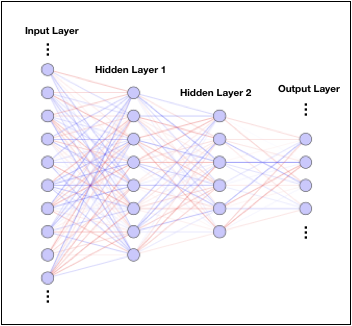
\includegraphics[scale=0.6]{nn-actor}
		\caption{Actor Network
			\label{nn-actor}}
	\end{figure}
	The Actor Network which approximate the policy $\pi_{\theta}(S)$ with parameter $\theta$ can be found in the above figure. It is a Neural Network with the following characteristics:
	\begin{itemize}
		\item Input Layer : The Input layer consists units with equal number to that of the dimensions of the state space. The Input is the observable state $S$. The Input Layer has a Rectified Linear Unit as its activation. Further the Input Layer is initialized with zero values for all its weights and biases. 
		\item Hidden Layers : The two Hidden layers consist of 32 and 16 neurons respectively. The hidden layers are fed from the output of th ReLU from the Input layers. Further each hidden layer has another ReLU as its activation. Both Hidden Layers are initialized with zero values for their weights and biases.
		\item Ouput Layer: The Output Layer consists of units with the same number as the dimension of the action space. The role of the output layer is to produce a probability distribution across the various possible actions so that we can choose the action with the highest probability. Thus we use a Softmax as the activation function which can generate the required distribution across the $n$ actions in the action space. The Output Layer is also initialized with zero values for all its weights and biases.
		\item Loss Function: here we use the Mean Squared Error loss function, from Equation \eqref{eq:mse_loss}.
		\item Optimizer: For the learning algorithm we have used the Adaptive Moments Optimizer (Adam)\cite{kingma2014adam} which is a special form of the SGD Algorithm where the learning rate adapts to the magnitude of the partial derivative of the cost function. 
	\end{itemize}
	\subsubsection{Critic Network}
	\begin{figure}[h]
		\vspace{0.2cm}
		\centering
		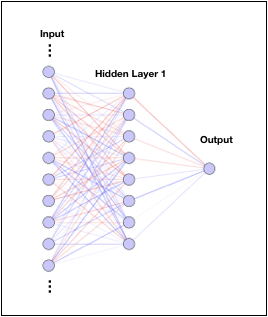
\includegraphics[scale=0.6]{nn-critic}
		\caption{Critic Network
			\label{nn-critic}}
	\end{figure}
	The Critic Network is a neural network that works to approximate the state-value function $\hat{v}_w(S)$ using parameters $w$ which represent its weights and biases. This can be found visually represented in the above figure. The Critic Network consists of Layers and Neurons, each with its own properties and functions. This is described below:
	\begin{itemize}
		\item Input Layer : The function of the Input layer here is to accept the current state $s_t$ of the dialog and feed it into the network. This layer consists of the same number of units as the dimension of the state space with the Input being the directly observable state. The Input Layer uses a Rectified Linear Unit for its activation and like the Actor Network, is initialized with zero values for all its weights and biases.
		\item Hidden Layer : The critic network since its job is simpler than the actor, uses only a single hidden layer with 16 Units. These units receive information from the Input layer. This single Layer has another ReLU as its activation and as before has all its parameters initialized with zeros.
		\item Output Layer : The Output layer of the critic network, since it has to produce a single value for the given state requires only a single neuron unit. The final magnitude that is produced by this isngle unit itself represents the \textit{value} of the given state and thus requires no activation. Further, this layer is also initialized with zeros.
		\item Loss Function : In the Critic Network we again use the Mean Squared Error loss.
		\item Optimizer : The Critic Network learns by using the previously discussed SGD Algorithm from Section \ref{sgd}.
	\end{itemize}
	% Please add the following required packages to your document preamble:
	% \usepackage{graphicx}
	
	
	\pagebreak
	\section{Experiments and Results}
	In this section we show how the implementation of the above discussed algorithms can be practical in developing simple dialog strategies. Further we discuss how these learning algorithms can be used together with a dialog MDP and a Simulated User to learn simple dialog strategies for the customer-support assistance domain. We also explore how the variation of  learning parameters such as the discount rate affect the resultant learned strategy. The purpose of these experiments is to show that it is possible to develop intelligent dialog systems in this domain and to reach an understanding of how these dialog strategies are affected by the learning framework. If we can establish this foundation then we could in the future extend this more realistic and practical situations with extremely large or continuous state-action spaces.
	\subsection{Overview}
	\subsection{Learning Simple Dialog Strategies}
	All learning algorithms and dialog environment/user simulation were all done using Python 3.6.6\cite{python}. Further we used Google Tensorflow\cite{tensorflow} and the Keras framework\cite{keras} to implement the neural network Approximators. These experiments have the following primary goals :
	\begin{itemize}
		\item To explore whether the implementation of the specific learning algorithms can indeed be useful and practical in its application to learning dialog strategies in this domain. Generally in the application of application of these algorithms the goal is generally easy to define but this is not the case with dialogs
		\item To explore how a variation in some learning parameters has an effect in the learning process, specifically the time to convergence on the learning curve and the quality of the resultant dialog strategy
		\item To compare the learning behavior of the various above algorithms compared to a baseline and compared to each other.
	\end{itemize}
	\subsubsection{Experimental Setup}\label{expt-setup}
	As discussed in Section \ref{dialog-mdp} our process of modeling the \textit{environment} is described as MDP which can be seen in \ref{chat-world3}. In dialogs modeled as a MDP, the observable state is directly the input received by the RL agent's \textit{Policy}. From Figure \ref{chat-world3} we can see that the entire system is composed of discrete states $S$, system actions $a$ and user utterances or responses $u$. The initial state of the system is always the same starting state that is automatically set every time the environment is reset. From here the system can perform actions as described below. These actions are then fed into the Environment Simulation which includes the user. According to this action the environment then queries the simulated user for a response. The joint probabilities of the current state $S_t$	and the previous action $a_t$ give the probability of transition in to the next dialog state which is fed back to the RL agent. The state transition model can be seen in Figure \ref{state-trans}. The simulation model is based on a simple state transition function of a probabilistic simulation environment similar to ones described in \cite{Singh_mdp}, \cite{walker2000evaluation} and \cite{roy2000spoken}. Thus in our framework both the model of state transition and the simulation environment are described by a single transition probability. Here the probability of the next state is given by the joint probability of the observation $o_t$, action $a_t$ at time $t$ and the state $s_{t+1}$ at time $t$. The observation here is noisy user input. Thus we have as the general state transition :
	\begin{align}\label{eq:trans-prob1}
	&P\big(s_{t+1},o_t | s_t\big) = P\big(s_{t+1} | o_t,a_t,s_t \big)\cdot P\big(o_t | a_t,s_t\big)\cdot P\big(a_t | s_t\big) \nonumber\\
	\end{align}
	Here we make the following assumptions
	\begin{itemize}
		\item We do not take into account noise that directly affects the choice of the action chosen. Thus the main job of the simulation becomes to evaluate the first and second term on the RHS of Eq \ref{eq:trans-prob1} while the last term depends on the learnt policy of the system.
		\item We assume that the output of the simulated environment and observation are directly representative of the state transitions
	\end{itemize}
	Thus we have :
	\begin{align}\label{eq:trans-prob2}
	P\big(s_{t+1}|o_t, s_t\big)
	= P\big(s_{t+1} | a_t, s_t\big) = P_{s,s'}^a
	\end{align}
	Thus the probability encodes the transition probabilities of the underlying MDP that represents the entire dialog and we do not need a complex dialog task model interpretation that is usually seen in literature, where this is job of some function approximator, usually a Recurrent Neural Network that takes as input the observation and returns an internal \textit{belief} state. This representation is also known as the Information State Paradigm \cite{Larsson:2000:ISD:973935.973943} which is characteristic of working with a full MDP.
	\begin{figure}[h]
		\centering
		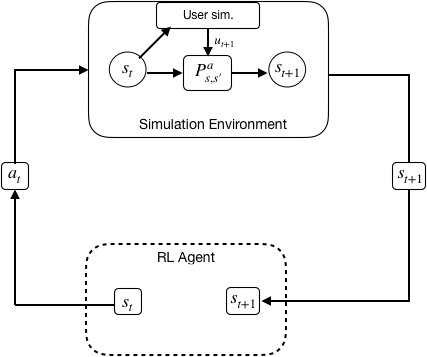
\includegraphics[scale=0.7]{state-trans}
		\caption{State Transition Model
			\label{state-trans}}
	\end{figure}
	Our environment as described above contains all components of the dialog system except the dialog management and learning module itself. This includes a probabilistic user model. Our simulated user is represented as a probabilistic model based on the recent interaction history. Thus the probability of generating user utterance $u_t$ at time $t$ is given by 
	\begin{align}
	\big(u_t | H_t\big)
	\end{align}
	Where $H_t$ represents the complete previous history of the dialog process. Here the history is given by the the previous system action and the previous dialog state which is representative of the chain of system actions and user utterances that occurred before the previous time step. Further we can assimilate the observation $o_t$ at time $t$ to be representative of this user response $u_t$ Thus our $P(o_t)$ from Eq.\ \ref{eq:trans-prob2} becomes
	\begin{align}
	&P\big(o_t | a_t, s_t\big)  = P\big(o_t | a_t, s_t, u_t\big).P\big(u_t | a_t, s_t\big)
	\end{align}
	Thus Equation \ref{eq:trans-prob2} becomes:
	\begin{align}\label{eq:trans-prob3}
	P\big(s_{t+1}|o_t, s_t\big).P\big(o_t | a_t, s_t, u_t\big).P\big(u_t | a_t, s_t\big) = P\big(s_{t+1},o_t,u_t | a_t, s_t\big)\nonumber\\
	= P\big(s_{t+1} | a_t, s_t\big) 
	\end{align}
	Finally the above equation \ref{eq:trans-prob3} represents our Dialog System state transition function as well as the transition probabilities of the underlying MDP. Further we can see an example of the probabilities in Table \ref{table:user-sim}. Here the topmost row represents the various discrete actions that the system is allowed to perform and the leftmost row represents the various states that the system can be in. The value for every state-action pair gives the probability of a \textit{positive} user response. Thus $\bar{P(a,s)}$ gives the probability of a \textit{negative} user response.
	\begin{table}[h]
		\caption{User Simulation Model}
		\label{table:user-sim}
		\resizebox{\textwidth}{!}{%
			\begin{tabular}{|l|l|l|l|l|l|l|l|l|l|l|l|l|l|l|l|}
				\hline
				& a1 & a2 & a3 & a4 & a5 & b1 & b2 & b3 & b4 & b5 & c1 & c2 & c3 & c4 & c5 \\ \hline
				s1 & 0.9 & 0.1 & 0.5 & 0.1 & 0.9 & 0.0 & 0.0 & 0.0 & 0.0 & 0.0 & 0.0 & 0.0 & 0.0 & 0.0 & 0.0 \\ \hline
				s2 & 0.0 & 0.0 & 0.0 & 0.0 & 0.0 & 0.5 & 0.9 & 0.1 & 0.1 & 0.9 & 0.0 & 0.0 & 0.0 & 0.0 & 0.0 \\ \hline
				s3 & 0.0 & 0.0 & 0.0 & 0.0 & 0.0 & 0.5 & 0.9 & 0.1 & 0.1 & 0.9 & 0.0 & 0.0 & 0.0 & 0.0 & 0.0 \\ \hline
				s4 & 0.0 & 0.0 & 0.0 & 0.0 & 0.0 & 0.5 & 0.9 & 0.1 & 0.1 & 0.9 & 0.0 & 0.0 & 0.0 & 0.0 & 0.0 \\ \hline
				s5 & 0.0 & 0.0 & 0.0 & 0.0 & 0.0 & 0.5 & 0.9 & 0.1 & 0.1 & 0.9 & 0.0 & 0.0 & 0.0 & 0.0 & 0.0 \\ \hline
				s6 & 0.0 & 0.0 & 0.0 & 0.0 & 0.0 & 0.5 & 0.9 & 0.1 & 0.1 & 0.9 & 0.0 & 0.0 & 0.0 & 0.0 & 0.0 \\ \hline
				s7 & 0.0 & 0.0 & 0.0 & 0.0 & 0.0 & 0.0 & 0.0 & 0.0 & 0.0 & 0.0 & 0.5 & 0.9 & 0.1 & 0.2 & 0.9 \\ \hline
				s8 & 0.0 & 0.0 & 0.0 & 0.0 & 0.0 & 0.0 & 0.0 & 0.0 & 0.0 & 0.0 & 0.5 & 0.9 & 0.1 & 0.2 & 0.9 \\ \hline
				s9 & 0.0 & 0.0 & 0.0 & 0.0 & 0.0 & 0.0 & 0.0 & 0.0 & 0.0 & 0.0 & 0.5 & 0.9 & 0.1 & 0.2 & 0.9 \\ \hline
				s10 & 0.0 & 0.0 & 0.0 & 0.0 & 0.0 & 0.0 & 0.0 & 0.0 & 0.0 & 0.0 & 0.5 & 0.9 & 0.1 & 0.2 & 0.9 \\ \hline
				s11 & 0.0 & 0.0 & 0.0 & 0.0 & 0.0 & 0.0 & 0.0 & 0.0 & 0.0 & 0.0 & 0.5 & 0.9 & 0.1 & 0.2 & 0.9 \\ \hline
				$s_{Tp}$ & - & - & - & - & - & - & - & - & - & - & - & - & - & - & - \\ \hline
				$s_{Tn}$ & - & - & - & - & - & - & - & - & - & - & - & - & - & - & - \\ \hline
			\end{tabular}%
		}
	\end{table}
	\clearpage
	\par
	The purpose of this first learned strategy will be to to offer the user a product recommendation(for a customer) and a following opening question for the user to ask said customer, according to this the system then suggests a offer or deal for the customer following which the system confirms the customers interest and closes the dialog, in this order. Thus the actions of the system or the \textit{Dialog Acts} can be in three separate classes corresponding to the above described stages of the conversation i.e.\  \textit{open}, \textit{offer} and \textit{close}. This can be seen in Table \ref{table:actions}. In the environment the actions are restricted to these three types i.e.\ \textit{opening\_question}, \textit{offer\_deal} and \textit{close\_deal}. The first action greets the user and offers a product to be recommended for his/her customer. If the customer responds positively then the system offers a deal for that customer, generally this would involve the querying of multiple knowledge sources. If this deal is accepted then the user can use a closing statement to confirm the deal and escalate the transaction to the billing department for example. The leftmost column in the table describes the type of action and the second column describes the number of action under this type. The actions are deigned to be favorable for different classes of users and the system is to learn to best sequences of actions to pick for a particular user class and recommendation.
	Further, as can be seen in Figure \ref{chat-world2} the number of possible responses from the user is restricted to two i.e.\ a positive and negative utterance to keep the system simple and to convey the needs of the user to the system. To represent the end of the dialog we have implemented Initial and Terminal States apart from the dialog states associated with the actual conversation. From Figure \ref{chat-world3} we can see that the system is always initialized to a starting state $S_0$ when the dialog starts and correspondingly the dialog ends when one of the two terminal states (represented by the bottom two boxes) are reached. These two terminal states represent respectively the situation where the dialog ended positively i.e.\ customer was interested in the offer and closed the deal or where the dialog ended negatively i.e.\ the customer was not interested in the recommendation or lost interest during the course of the dialog with the user. These two terminal states are represented by $S_{Tp}$ for a positive end to the episode and $S_{Tn}$ for a negative end. The final landing of the system in one these two terminal states also controls the rewards associated with each dialog episode. Here $T$ represents the final time-step of an episode i.e. each episode consists of time-steps $1, 2, 3, \ldots T$ Unless mentioned otherwise all experiments have the reward function described as:
	\begin{align}
	R = \begin{cases}
	1 & \text{if }S_T = S_{Tp} \\    
	0 & \text{if }S_T = S_{Tn}
	\end{cases}\label{reward_func}
	\end{align}
	Thus the system get a positive unit reward if the final state is positive and no reward otherwise. Keeping the reward simple allows us to accurately define and measure the rate of task completion and thus optimize on this completion rate only which allows us to converge on the best sequence of system actions to which most users would respond positively. Here the task completion rate is the ratio of dialogs ending with $R = 1$.%[Create full table like the one found in file:///Users/shishir/Documents/Thesis%20Stuff/Surveys%20and%20Frameworks/A%20Comprehensive%20RL%20Framework%20for%20Dialogue%20Management%20Optimisation.pdf] pg 6 fig 1
	\begin{table}[H]
		\caption{System Actions}
		\centering
		\label{table:actions}
		\resizebox{\textwidth}{!}{%
			\begin{tabular}{|l|l|p{5cm}|p{5cm}|}
				\hline
				System Actions     & \# & Description                                                                                                     & Example                                                                                                                                    \\ \hline
				opening\_question  & 5  & Opens the sales conversation by asking a product related sales question                                         & Do you store many valuables at home?                                                                                                       \\ \hline
				offer\_deal        & 5  & Offers a customer and product specific deal                                                                     & We offer one of the cheapest Household Liability Insurance on the market currently, you can offer a discount of 15\% for the first 1 year. \\ \hline
				closing\_deal & 5  & Closes the deal and gets an idea of the escalation direction. Could also start a new dialog for another product & Is the customer interested in going forward or would he like to know more?                                                                 \\ \hline
			\end{tabular}%
		}
	\end{table}
	\subsubsection{Learning with A2C}
	The goal of this  first learned policy is, as discussed above to greet and recommend a product and opening question to the user, followed by presenting a offer/deal and ending the dialog by closing said offer. A single experiment lasts 5000 episodes and the resulting rewards for each episode are collected and smoothed by taking the mean and displayed for comparison. This forms the learning curve for that algorithm. In order to clearly comprehend the various aspects of the A2C learning algorithm a comparison is made with two standard algorithms which we use as baselines. These are SARSA and Q-learning \cite{Sutton-introRL} and were chosen as they are the most commonly applied RL algorithms. Here the Q-learning algorithm is generally off-policy but can be used with either offline and online approaches. The SARSA algorithm is representative of an on-policy and online technique. The representation of the Q-function (state-value function) in this baseline implementation is linear and non-parameterized i.e.\ we do not use any function approximator such as a neural network but a simple table to hold Q-values. Please check Section \ref{a2c-section} for a detailed view on the Advantage Actor Critic formulation.
	
	\myparagraph{Results}
	The learning curves are formed by performing at least 5000 episodes and learning is evaluated by taking the average return over at least 5 experiments. There are many parameters to be initialized, these are given below:
	\begin{enumerate}
		\item SARSA Hyperparameters:
		\begin{itemize}
			\item $\epsilon$-Greedy value = 0.1
			\item Discount Factor $\gamma_{SARSA}$ = 0.98
			\item Learning Rate $\alpha_{SARSA}$ = 0.01
		\end{itemize}
		\item Q-learning Hyperparameters:
		\begin{itemize}
			\item $\epsilon$-Greedy value = 0.1
			\item Discount Factor $\gamma_{Q-learning}$ = 0.98
			\item Learning Rate $\alpha_{Q-learning}$ = 0.01
		\end{itemize}
		\item A2C Hyperparameters:
		\begin{itemize}
			\item Discount Factor $\gamma_{A2C}$ = 0.98
			\item Actor Network Learning Rate $\alpha_{Actor}$ = 0.01
			\item Critic Network Learning Rate $\alpha_{Critic}$ = 0.01
			\item Actor Network Layers : 3 Hidden layers with 32, 64 and 32 units respectively.
			\item Critic Network Layers : 1 Hidden layer with 64 units.
		\end{itemize}
	\end{enumerate}
	These parameters were defined as the result of a large amount of tuning, these parameters sets are based on two criteria, the system must reach highest possible returns and second the speed of learning. The above described parameter sets were found to be the best for the above described (Section \ref{expt-setup}) experimental setup. 
	\begin{figure}[H]
		\hspace*{-2cm}   
		\centering
		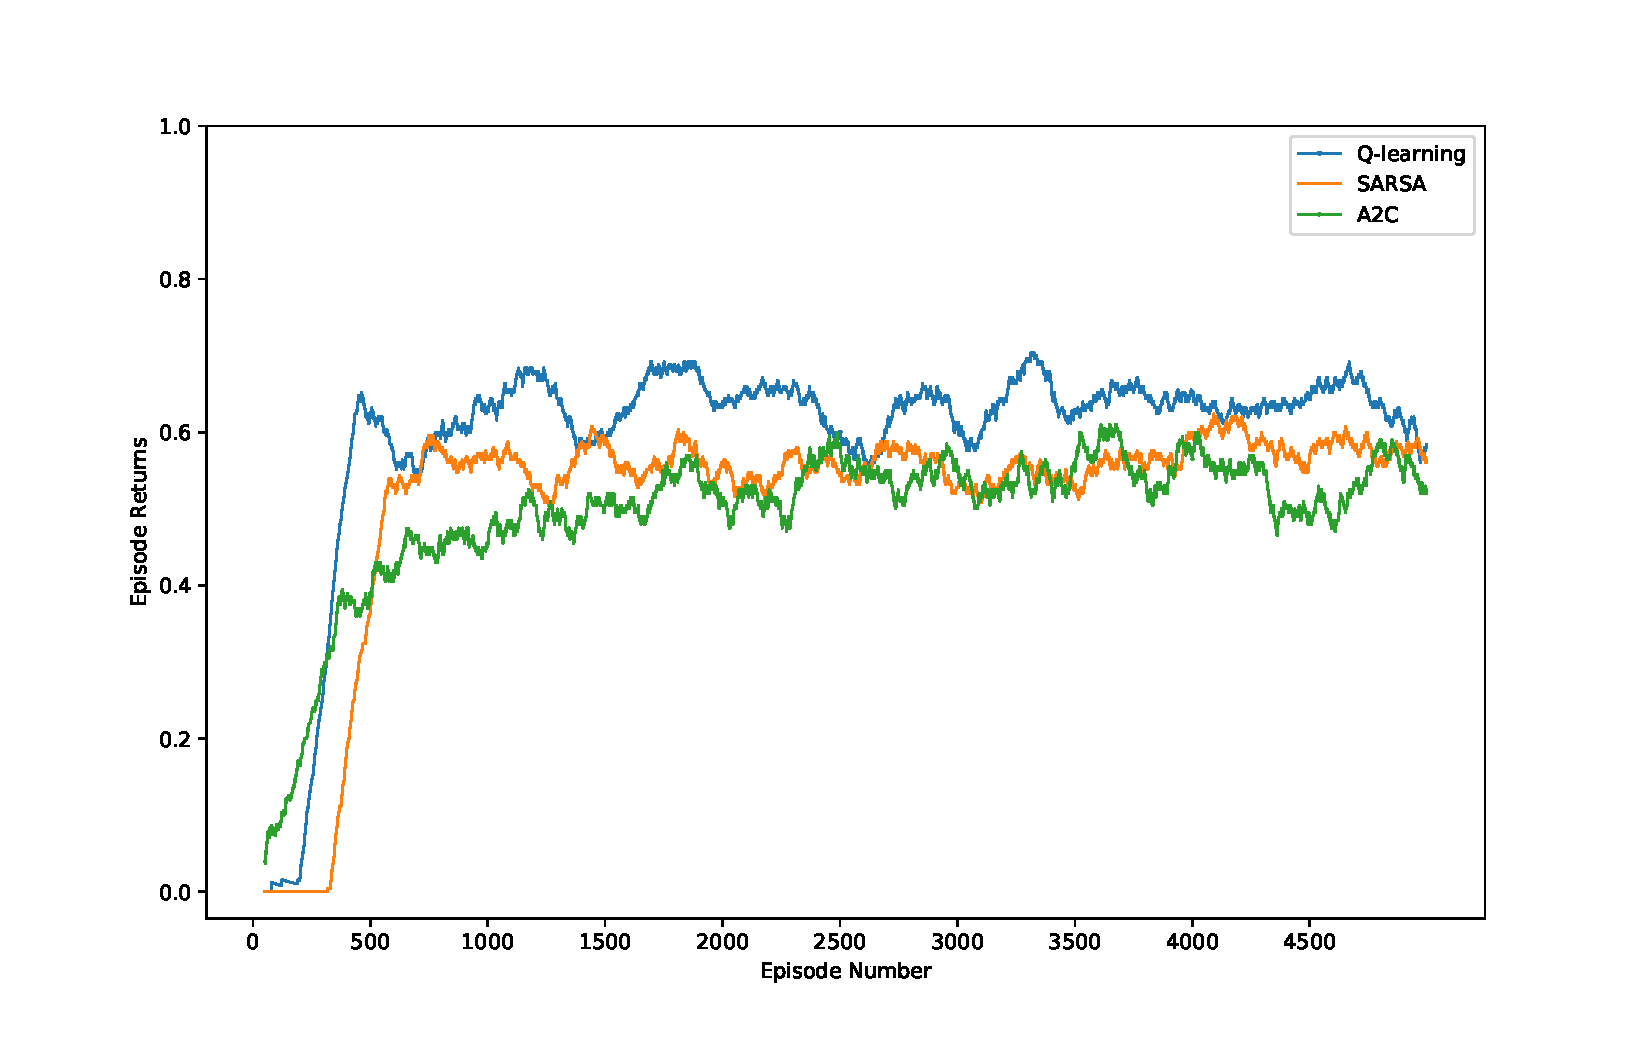
\includegraphics[scale=0.7]{plota2c_250_3.pdf}
		\caption{A2C Learning Curve
			\label{a2c-plot}}
	\end{figure}
	The learning curve for this experiment can be see in Figure \ref{a2c-plot}. Here the the individual curves are smoothed by the method of moving averages with a rolling window of 200 data points. We can infer from the plot that the A2C algorithm successfully learns the required dialog strategy and converges to the maximum return path or optimal policy after around 500 episodes. Compared to the two baseline algorithms, it seems that A2C converges faster with fewer training episodes. 
	First, from the graph we can see that the A2C algorithm is the first to hit the maximum return for an episode after just around 50 episodes and its curve immediately starts to improve as the returns from these steps are incorporated into the policy and value networks. In contrast we can see that Q-Learning and SARSA take at least 250 - 750 episodes to start improving, presumably this could be due to the $\epsilon$-greedy behavior in these algorithms that restrict the exploration phase and extend the exploitation phase. The returns during these first 500 episodes for SARSA and Q-learning, would have been 0 but the system learnt that this must be most optimal. Due to this and the low rate of $\epsilon$ most greedy actions did not result in an improvement of the returns. This changed when $\epsilon$ finally allowed the system to explore the paths with most return around episode 500. This problem was avoided with A2C as it, according to the input state, chooses actions directly from a probability distribution across the different actions i.e.\ softmax output from the Actor/Policy Network and does not follow $\epsilon$-greedy behavior. Further, the fluctuations that can be seen in SARSA and Q-learning where the curve takes a periodic dip in the return can also be attributed to the forced exploration that $\epsilon$ controls which would disturb the policy from picking the action. Further, we can infer from the graph that for relatively small state-action spaces, tabular methods such as SARSA and Q-Learning perform almost 15 - 20\% better after 1000 episodes than a parameterized policy method such as A2C. The sudden increase in performance of SARSA and Q-learning between 250 to 500 episodes shows that value based methods are indeed more sample efficient than policy methods.
	\myparagraph{Effect of the Discount Factor}\label{a2c_df_effect}
	For the A2C Algorithm and typically in RL we have an addition hyperparameter called the \textit{discount factor} denoted by $\gamma$. The system is simulated using a few variants of $\gamma$ while keeping the other parameters such as the actor learning rate $\alpha_{Actor}$, critic learning rate $\alpha_{Critic}$ and the number of layers in both networks constant. 
	\begin{figure}[H]
		\hspace*{-3.25cm}   
		\centering
		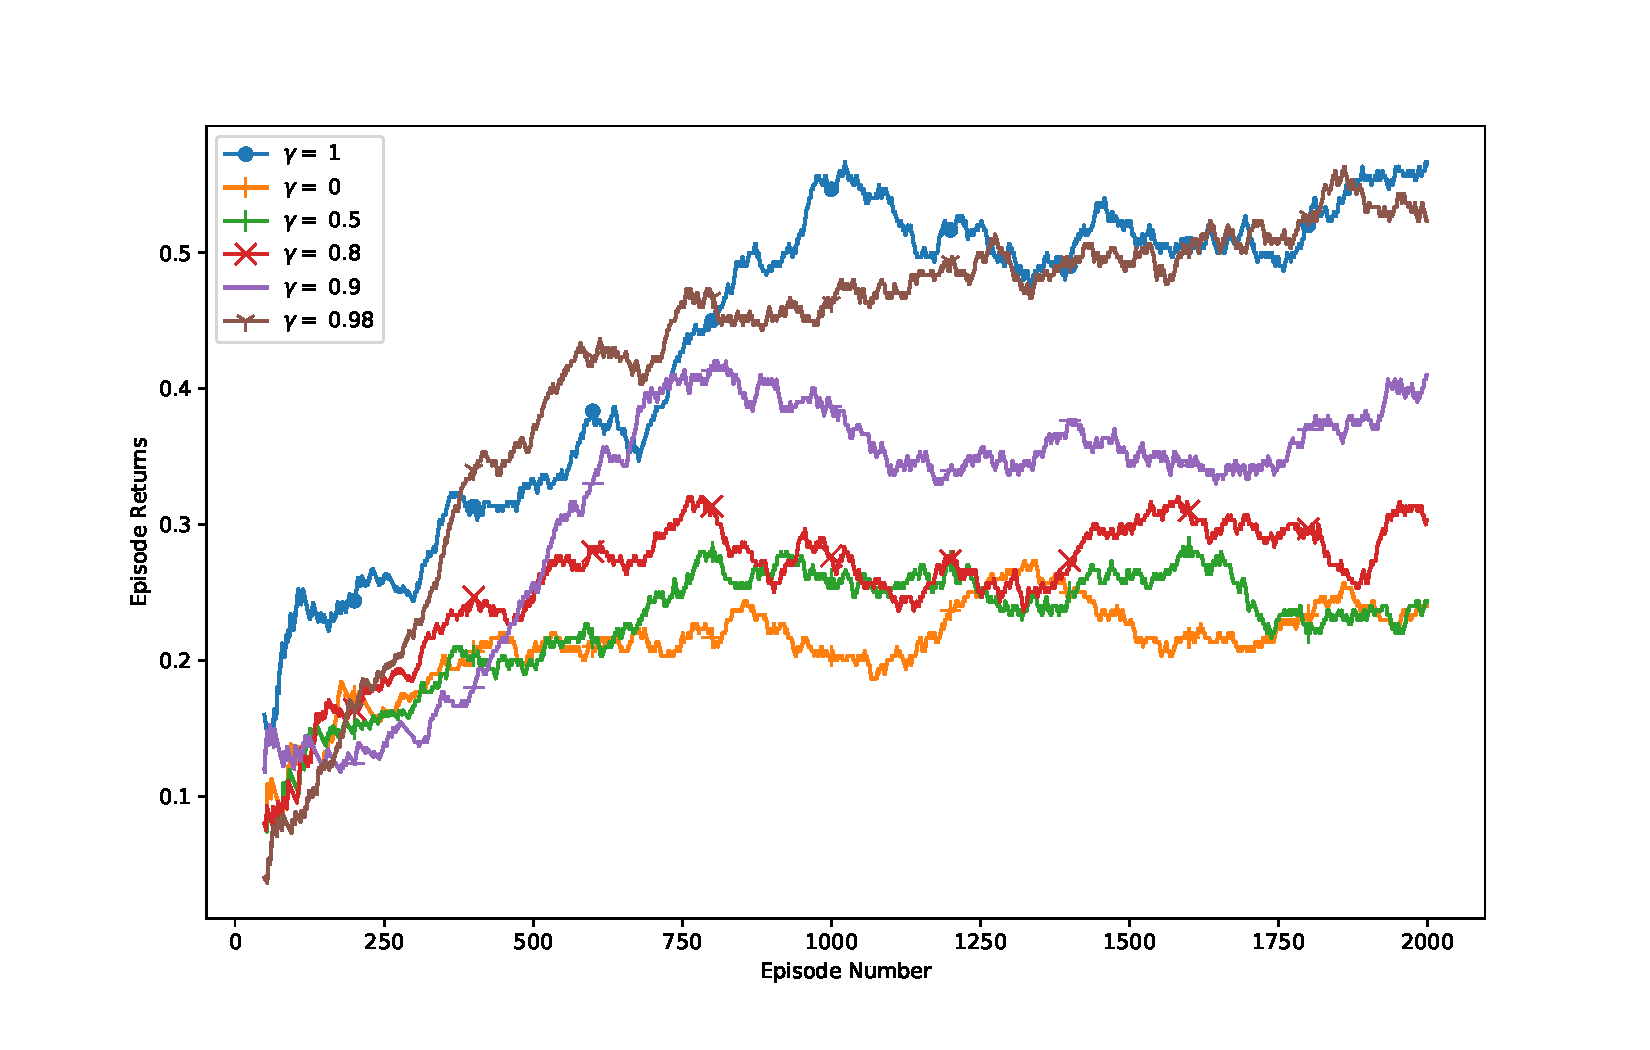
\includegraphics[scale=0.8]{a2c-dis-fact.pdf}
		\caption{Effect of the Discount Factor on A2C Learning
			\label{a2c_dis_fact}}
	\end{figure}
	The influence of the discount factor also known as the forgetting factor $\gamma$ can be seen in Figure \ref{a2c_dis_fact} where the smoothed average episodic return is plotted against the number of episodes. The amount of information in each update of the Actor and Critic Network weights is directly influenced by the discount factor $\gamma$. Intuitively this means the agents behavior is affected by making it prefer long-term rewards than short-term or even immediate rewards. This becomes important in our scenario where the agent only receives a reward at the final step of the episode and so must optimize the preceding steps so as to reach the correct final step. If $\gamma = 0$ or close to 0 then this means that the agent is very \textit{short-sighted} and does not consider any rewards other than the most immediate one, in contrast if $\gamma = 1$ then the agent considers all rewards that it may receive in the following steps. This is observed in the given diagram, where the performance beings to degrade as we bring the discount factor closer to 0. We can also notice that the discount factor does not seem to have a large affect on the speed of convergence since the gradient of the best performing curve ($\gamma > 0.9$) converges after 1000 episodes so does the worst performing curve ($\gamma \leq 0.5$) around the same episode. Another interesting phenomenon is that the discount rate seems to critically effect a rise in performance only on the upper bound close to 1 or $\gamma > 0.9$, this can be seen the curves for $\gamma \leq 0.8$ which seem to show a low but similar performance with respect to each other. As we move $\gamma$ upward by just $0.1$ we get almost a two fold increase in performance. This again can be attributed to the fact that we have very delayed rewards in our environment and only at the last step, this would require the agent to be very long-sighted to be able to push the policy gradient toward this maximum return region that would only occur 3 or 4 time-steps following the starting state if following an optimal path.
	
	\myparagraph{Effect of Reward Magnitude}
	This third set of experiments is to examine how varying the absolute magnitude of the reward $R$. The system was simulated using the same reward structure i.e.\ one positive final reward signal at the end of each successful episode but varying the absolute magnitude of this reward unit by a factor of 10. Thus we tested the learning curve for $R = 1, 10, 10^2, 10^3$ and $10^4$.To do this we kept all other hyperparameters such as the actor learning rate $\alpha_{Actor}$, critic learning rate $\alpha_{Critic}$ , discount factor $\gamma$, $\epsilon$ and the number of layers in both networks as constant. The effects of varying the reward in this way can be seen in Figure \ref{a2c_reward_mag} where we plot the absolute magnitude in the log scale on the y axis vs the number of episodes on x. The curves have been smoothed by using the method of moving averages with a rolling window of 200 data points. Each experiment ran for 5000 episodes and the resultant learning curve was built from the average of 5 repetitions. 
	\begin{figure}[H]
		\hspace*{-3.25cm}   
		\centering
		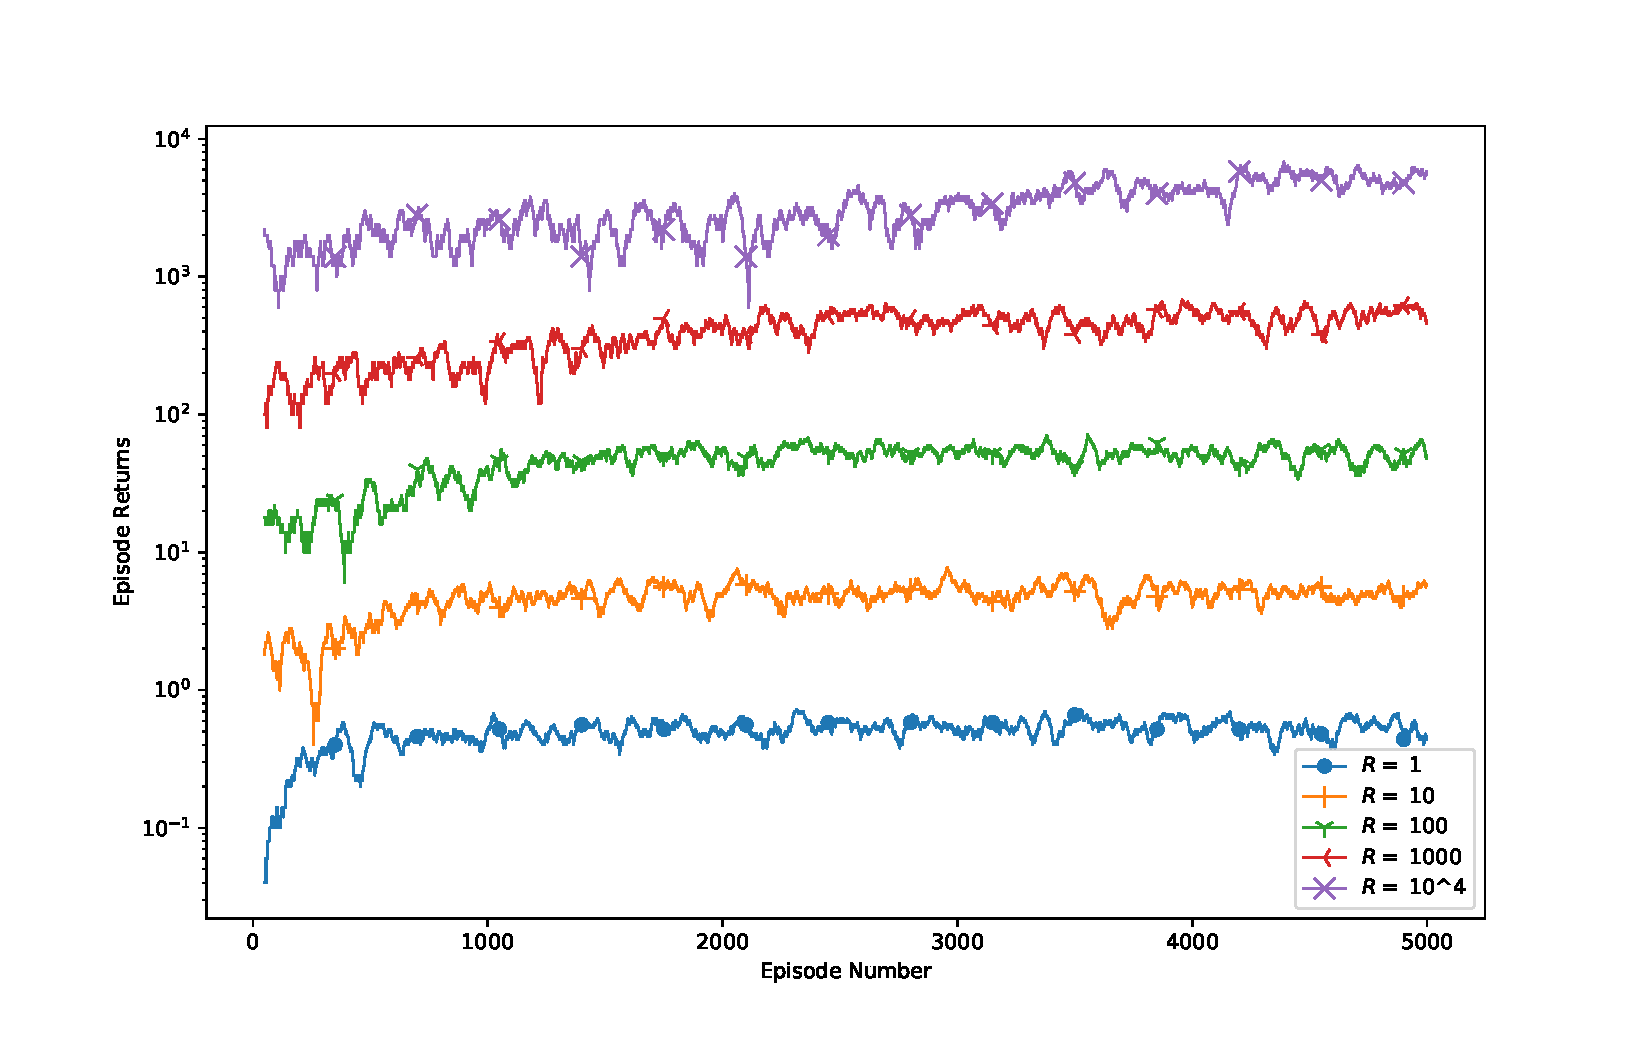
\includegraphics[scale=0.8]{a2c_reward_mag.pdf}
		\caption{Effect of the Absolute Reward Magnitude on A2C Learning
			\label{a2c_reward_mag}}
	\end{figure}
	According to the learning curves it is observed that reward magnitude does not significant seem to affect the performance of the final learnt dialog but does seem to have a small effect on the learning speed. As we can see the gradient of the curve for $R = 1$ converges after about 400 episodes, but as we increase the magnitude of the reward 10 fold we can see that, for the same performance the convergence now requires around 900 episodes. Similar behavior can be seen in the other curves with $R \geq 100$ where we now need atleast $ 1000 - 1200$ episodes to converge. This shows that that lower rewards are a little bit more sensitive to updates, but this could also be due to statistical fluctuations.
	\subsubsection{Learning with REINFORCE}
	Similar to the experiments conducted with the A2C Algorithm, here we attempt to use the REINFORCE algorithm to learn the dialog strategy discussed in Section \ref{expt-setup}. Here each experimental run lasted 5000 episodes with the total returns from each episode being collected to form the learning curve shown below. To gain a better understanding of learning with REINFORCE we again use SARSA and Q-learning\cite{Sutton-introRL} as baselines. As we know the SARSA is online while Q-learning is offline and uses a simple table to hold the Q values. Please see Section \ref{reinforce} for a detailed explanation of the REINFORCE process. it should be noted here that for these set of experiments we modify the reward function from Equation \ref{reward_func} to 
	\begin{align}
	R = \begin{cases}
	10 & \text{if }S_T = S_{Tp} \\    
	0 & \text{if }S_T = S_{Tn}
	\end{cases}\label{reward_func_10}
	\end{align}
	\myparagraph{Results}\label{reinf_pre_results}
	The Hyperparameters for the experiments were initialized as shown below.
	\begin{enumerate}
		\item SARSA Hyperparameters:
		\begin{itemize}
			\item $\epsilon$-Greedy value = 0.2
			\item Discount Factor $\gamma_{SARSA}$ = 0.9
			\item Learning Rate $\alpha_{SARSA}$ = 0.01
		\end{itemize}
		\item Q-learning Hyperparameters:
		\begin{itemize}
			\item $\epsilon$-Greedy value = 0.2
			\item Discount Factor $\gamma_{Q-learning}$ = 0.9
			\item Learning Rate $\alpha_{Q-learning}$ = 0.01
		\end{itemize}
		\item REINFORCE Hyperparameters:
		\begin{itemize}
			\item Discount Factor $\gamma_{reinforce}$ = 0.9
			\item Policy Network Learning Rate $\alpha_{Actor}$ = 0.01
			\item Policy Network Layers : 2 Hidden layers with 10 and 10 units respectively.
		\end{itemize}
	\end{enumerate}
	Based on a large number of training iterations and consequent tuning, the above parameters were found to produce the highest returns and fastest training times. Thus they were found to be the best set of parameters for the above described experimental setup (Section \ref{expt-setup}).
	\begin{figure}[H]
		\hspace*{-3.25cm}   
		\centering
		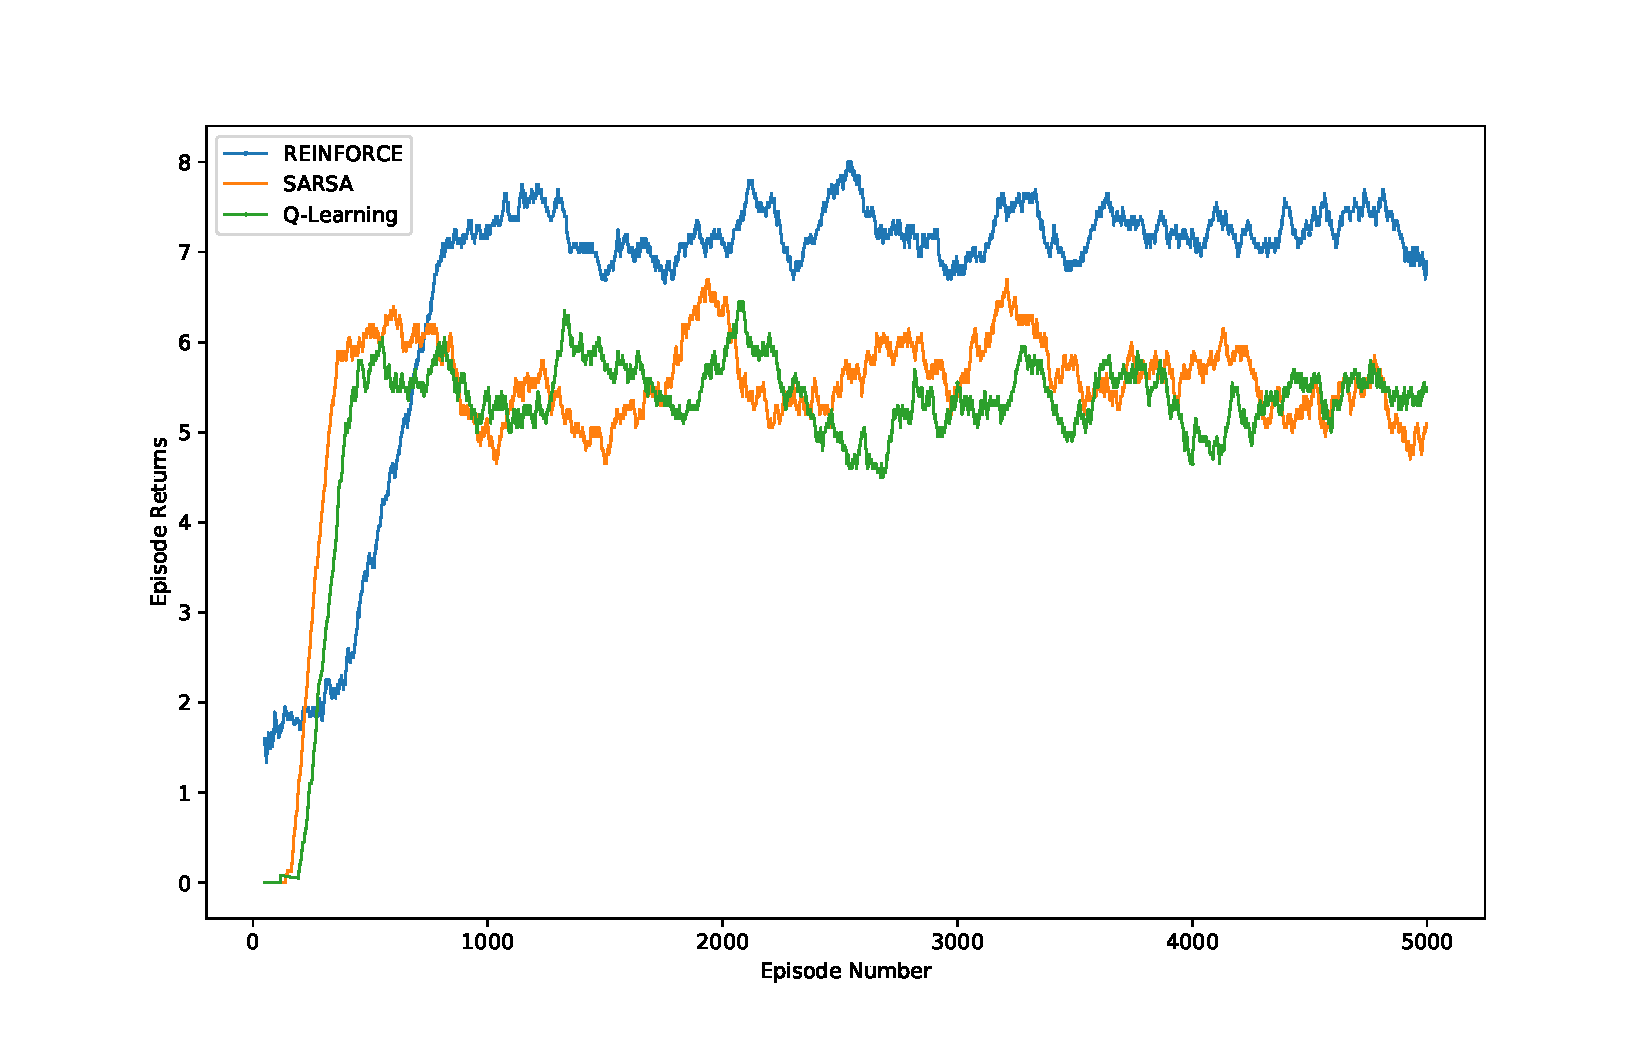
\includegraphics[scale=0.8]{plot_reinforce_250.pdf}
		\caption{REINFORCE Learning Curve
			\label{reinforce-plot}}
	\end{figure}
	The learning curves are plotted in Figure \ref{reinforce-plot}. Here each curve was smoothed by the method of moving averages with a rolling window of 200 data points. From first glance we can see that REINFORCE does indeed converge to a policy with highest returns after 800 episodes. When we compare it to the two baselines we can see that it shows a much higher performance but slower training times. We can also see that REINFORCE is the last to converge while Q learning and SARSA converge  faster, taking only about 300 episodes to do so. This is because \textit{vanilla} Policy Gradient methods such as REINFORCE, suffer from a high degree of variance. This variance stems from the fact that the policy update defined by $\nabla_{\theta}J(\theta)$ varies depending on the trajectories or path the system takes through the MDP. From Equation \ref{eq:pg-expectation} we have $\nabla_{\theta}J(\theta)=\mathbb{E}_{\pi}\big[\sum_{a}q_{\pi}\big(s_t,a\big)\nabla_{\theta}\pi_{\theta}\big(a|s_t\big)\big]$. Here we can see that both the terms are dependent on the \textit{current} action and state from the path that the system is following. In REINFORCE recall that we compute this gradient by sampling trajectories from the policy i.e.\ $a \sim \pi_{\theta}(s)$ and then average over them to get the expectation (for each episode). Thus the gradient is dependent on the current actions and states. This causes high variance as these trajectories can take very different paths which means that the two terms in the above equation $q_{\pi}\big(s_t,a\big)$ and $\nabla_{\theta}\pi_{\theta}\big(a|s_t\big)$ can take very different values according to the path it follows. This makes it is difficult for this algorithm to find the value of its states and affects the performance. Once it has visited states of relatively high value(local optima) it repeatedly optimizes the same policy without further exploration of the state-action space, this is the cause behind the better performance of REINFORCE. SARSA and Q learning on the other hand could depend on the values they assigned to the state action pairs as these algorithms optimize the value function itself and not the policy as REINFORCE. The $\epsilon$-greedy process let the baselines to explore further and reach the states with associated with the highest returns after about 500 episodes. Once these states were assigned high values, due to the high return, they were easily  able to converge to the optimal path by repeatedly visiting those states. Thus we can infer from the plot that for small state-action spaces and without an approach to reduce the variance for REINFORCE such as using an intrinsic baseline (such as A2C), tabular methods such as SARSA and Q-learning converge faster but REINFORCE shows a much higher performance for the same task.
	
	
	\subsection{Summary}
	In summary we can say confidently that both the REINFORCE and Advantage Actor-Critic Algorithms can be used to learn dialog strategies for our domain, where our environment is modeled as a full MDP. In these experiments we saw that the learned policies shows behaviors that are fully in conjunction with our simple simulated environment and user. Thus these experiments have been fundamental in helping us understand and answer questions of what can be done with the employed algorithms and how we could go about using and applying them to domain specific features and goals. However, in this setup the state-action space is very small and limited. Now we need to scale up to more realistic scenarios that require a Partially Observable MDP and much larger state-action spaces.
	\clearpage
	\section{Conclusions}
	\subsection{Conclusion}
	In this work we have seen that RL provides an excellent framework for general decision making tasks. Further, we have seen that this is useful for the development of automated dialog policy learning systems. In this thesis we have shown that these two algorithms can address the challenge of learning dialog that is designed as complete Markov Decision Process.
	In general with this work we have also explored in-depth the concept of Domain Specific or Goal-Oriented dialog systems which are based on Reinforcement Learning. Further we examine the fundamental concepts involved in RL such as a MDP and the various basic methods and techniques to solve them. We have also studied and shown the required mathematical tools and structures such as MLPs, loss functions and deep learning in general to help us overcome the challenges present in developing dialog systems.
	Further, We show that the Policy Based RL methods such as REINFORCE and Advantage Actor-Critic can indeed be used in the developing of Goal-Oriented Dialog Systems in the domain of sales assistance and explore in-depth the working behind these algorithms and how we would implement these algorithms using deep neural networks. With repeated experimentation we also give the best set of hyperparameters that encourage learning of optimal dialog policies using these algorithms. Finally we show the advantages in using these algorithms and the difference in learning behaviors compared to standard baselines such as SARSA and Q-Learning.
	\subsection{Future Work}
	Based on the work done in this thesis and the consequent conclusions above we discuss a few further possibilities and future extensions :
	\begin{itemize}
		\item Extend the environment to include noisy real user input. This would introduce partial observability of our currently full MDP and also a Natural Language Understanding Unit due to the need to recognize and classify input speech dialog acts which would also introduce speech recognition errors due to the noise in user input and the quality of the NLU module. From here one would have to model the environment as a POMDP\cite{Sutton-introRL}. This stems from the fact that the dialog manager (which includes the NLU) may not be able fully understand what is input by a user, and thus the dialog states must be made more complex, perhaps with a so called \textit{confidence score} for different dialog state features to differentiate the multitude of states. This is also describes above as Discriminative dialog state tracking.
		\item Since our User simulation was on based a simple joint probability based on the history of the dialog, future work should extend this to include multiple complex users each with the their own goals and agenda. Perhaps using a complex probabilistic model based on Hidden Markov Models.
		\item Extend to a more complex reward function that better encodes the true rewards in more realistic human machine interaction situations. For tasks such as our which aim to assist the user with some goal the reward function can be extended to be more appropriate learning the required policies, step rewards for positive user utterances, punishing extended dialog with a lot of turns etc. Further the complex reward modeling for these tasks has received relatively less research attention and is thus remains a big challenge for developing robust dialog systems. Thus it may be important to continue research in the direction of complex reward modeling.
		\item Testing the use of further sophisticated RL approaches such as Deep Q Networks, Generative Adversarial Networks and Deep Deterministic Policy Gradients in the development of robust dialog systems
	\end{itemize}
	
	\clearpage
	\section[References]{Bibliography}
	\bibliographystyle{apa}
	\bibliography{references}
	
\end{document}

